\documentclass{article}

\usepackage[style=authoryear, backend=biber]{biblatex}
\addbibresource{../references.bib}
\addbibresource{method.bib}
\usepackage[a4paper, total={6 in, 9 in}]{geometry}

\usepackage{mathtools}
\usepackage{graphicx}
\usepackage{subcaption}
\usepackage{caption}
\usepackage{booktabs}
\usepackage{adjustbox}
\usepackage{multirow}
\usepackage{caption}
\usepackage{eurosym} 
\usepackage{xcolor}
\usepackage{comment}
\usepackage{subcaption}
\usepackage{amssymb, amsmath}
\usepackage{algorithm}
\usepackage{algpseudocode}
\usepackage{blindtext}
\usepackage{pdflscape}
\usepackage{rotating}
\usepackage{longtable}
\usepackage{placeins}
\usepackage{spverbatim}
\usepackage{tikz}
\usepackage{rotating}
\usepackage{pgfplots}
\pgfplotsset{width=10cm,compat=1.9}

\usepackage{makecell}
\usepackage[flushleft]{threeparttable}
\renewcommand\theadalign{bc}
\renewcommand\theadfont{\bfseries}
\renewcommand\theadgape{\Gape[4pt]}
\renewcommand\cellgape{\Gape[4pt]}
\usepackage{tikz}
\usepackage{tikz-3dplot}

\usetikzlibrary{shapes,shapes.geometric, positioning, fit, backgrounds, calc, 3d, shapes.multipart, arrows.meta, patterns, perspective}

\newcommand\lbo{0.5}
\newcommand\wbo{1}
\newcommand\hbo{1}
\newcommand\lbt{2}
\newcommand\wbt{1}
\newcommand\hbt{1}
\newcommand\separationofcircles{0.1}


\tikzset{
    single_redbox/.pic={
    \draw[red, dashed, opacity=0.5] (0-\lbo,0-\wbo,0-\hbo) -- ++(0,0,\hbo);
    \draw[red, dashed, opacity=0.5] (0-\lbo,0-\wbo,0-\hbo) -- ++(0,\wbo,0);
    \draw[red, dashed, opacity=0.5] (0-\lbo,0-\wbo,0-\hbo) -- ++(\lbo,0,0);
    
    % Draw front faces
    \draw[red, fill=red!20, opacity=0.5] (0,0,0) -- ++(-\lbo,0,0) -- ++(0,-\wbo,0) -- ++(\lbo,0,0) -- cycle;
    \draw[red, fill=red!30, opacity=0.5] (0,0,0) -- ++(0,0,-\hbo) -- ++(0,-\wbo,0) -- ++(0,0,\hbo) -- cycle;
    \draw[red, fill=red!40, opacity=0.5] (0,0,0) -- ++(-\lbo,0,0) -- ++(0,0,-\hbo) -- ++(\lbo,0,0) -- cycle;
    }
}
\tikzstyle{line} = [draw, -Latex]

\newcommand{\neworrenewcommand}[1]{\providecommand{#1}{}\renewcommand{#1}}

\newcommand{\drawblock}[9]{
    \neworrenewcommand{\ffoo}[1]{
           
        \foreach \i in {0,...,#8} {
            \foreach \j in {0,...,#9} {
                \foreach \k in {0,...,##1} {
                    % Only draw the visible faces
                    % Front face
                    \ifnum \i=#8
                        \draw[#7, fill=#7!50] (#1+\i*#4+#4,#2+\j*#5,#3+\k*#6) -- ++(0,#5,0) -- ++(0,0,#6) -- ++(0,-#5,0) -- cycle;
                    \fi
                    % Right face
                    \ifnum \j=#9
                        \draw[#7, fill=#7!30] (#1+\i*#4,#2+#5+\j*#5,#3+\k*#6) -- ++(#4,0,0) -- ++(0,0,#6) -- ++(-#4,0,0) -- cycle;
                    \fi
                    % Top face
                    \ifnum \k=##1
                        \draw[#7, fill=#7!20] (#1+\i*#4,#2+\j*#5,#3+#6+\k*#6) -- ++(#4,0,0) -- ++(0,#5,0) -- ++(-#4,0,0) -- cycle;
                    \fi
                    % Draw a point at each vertex
                    % \fill (#1+\i*#4,#2+\j*#5,#3+\k*#6) circle (1pt);
                }
            }
        }
    
    }
    \ffoo
}



      \tikzset{
    box/.style={rectangle, draw, fill=gray!20, align=center, minimum height=1cm, minimum width=2.5cm},
    ellip/.style={draw, ellipse, align=center, minimum width=2.5cm, minimum height=1cm},
    label_node/.style={circle, draw, fill=#1, text=black, inner sep=1pt, minimum size=1em, font=\bfseries},
    gene_node/.style={ align=center, inner sep=2pt, fill=white, minimum width=0.5cm, minimum height=1cm},
    gene_group/.style={rectangle, draw, inner sep=6pt, rounded corners, align=center, minimum height=2.5cm},
    aux_gene_group/.style={align=center, inner sep=2pt, minimum width=2cm, minimum height=1cm}
  }

\providecommand{\keywords}[1]
{
  \small	
  \textbf{\textit{Keywords---}} #1
}

% Visible marker for a number or table that does not exist yet.  Every use is
% a place where a generated fragment or a regenerated run must supply the
% value; grep for \pending before submitting.
\providecommand{\pending}[1]{\textcolor{red}{\textbf{[pending: #1]}}}
\providecommand{\pendingcell}{\textcolor{red}{\textbf{[pending]}}}
\usepackage{amsthm}
\newtheorem{proposition}{Proposition}

\usetikzlibrary{decorations.pathreplacing}

% A number that a campaign in progress will replace.  It prints its argument,
% so the paper builds and reads normally; every use is listed with its
% replacing campaign in rewrite/inflight-sites.md.
\providecommand{\InFlight}[1]{#1}

\title{An optimisation approach for supply chain procurement transport
operational planning with 3D full-truckload constraints and returnable
transport items}
\date{}

\newenvironment{ChapterAppendix}{\appendix}{}

\begin{document}
\maketitle

In procurement transport planning with returnable transport items
(RTIs) --- foldable containers that must be returned empty --- the
delivery and the return flow are each other's supply. We formulate
3D-SCPTOP, a mixed integer programme joining the transport and
inventory decisions to a full-truckload condition stated as a 3D
loading problem: RTIs form vertical stacks under a height budget and a
per-stack crush limit, whose footprints must be placed on the trailer
floor without overlap. The formulation is written over trucks, so it
is block-angular over (direction, truck, period); deleting that
quantifier yields the pricing problem of a Dantzig--Wolfe
reformulation whose master carries \emph{no} loading configuration. We solve it with BP-3D-SCPTOP: branch and price over
the fleet vector, with a flow-first relax-and-fix construction as
primal heuristic and a lower bound certified on the volumetric
relaxation, valid for the 3D problem by inclusion. The branching
hierarchy is finite and complete, so the procedure is exact given
compute; what it reports here is an incumbent verified truck by truck
against its own layout, a certified bound, and no proof of optimality.
On thirty-six generated instances
it returns a verified plan on thirty-one, at a mean certified gap of
$8.8\%$ over thirty of them; on four size-ladder instances a compact 3D formulation
returns a plan only on the smallest, of five periods. Of the $724$
truck loads a volumetric capacity model dispatches on those instances,
$501$ ($69.2\%$) are \emph{proved} impossible to place in a trailer.

\keywords{Procurement transport planning, inventory, returnable
transport items, full-truckload, 3D container loading, branch and price}

\section{Introduction}
\label{sec:intro}

Taking transport, inventory and production decisions jointly improves
supply chain performance \autocite{Stadtler2015SupplyPlanning,
Diaz-Madronero2017ADecisions}. Responsibility for transport planning
usually lies with the supplier
\autocite{Fleischmann2015TransportDistribution}, but in the automotive
industry the manufacturer frequently plans its own inbound transport,
and it does so around an asset material requirements planning does not
represent: the returnable transport item (RTI), the tertiary packaging
in which parts move. The plant returns folded empty RTIs and the
supplier sends them back erected and full, so each flow is the other's
supply and neither can be planned alone. Algorithm-based planning
outperforms a planner's intuition here
\autocite{Diaz-Madronero2014AChain}, most where intuition is weakest:
deciding how many trucks to dispatch when whether a given set of
containers fits inside one is itself a combinatorial question.

That last question is the one the literature does not ask. Transport
capacity in procurement transport planning is a scalar --- freight
volume, or a count of loaded units
\autocite{Hashemi-Amiri2023IntegratedApproach,
Diaz-Madronero2014AChain} --- but containers are not fluid: they stack
in whole layers under a height budget and a crush limit, and their
footprints tile a floor in whole rectangles. A plan drawn against a
volumetric capacity can therefore prescribe loads that no arrangement
of the trailer admits, and the shortfall is discovered on the loading
dock rather than in the model.
Section~\ref{sec:res-abstraction} measures how often, by placeability
proof rather than by argument.

This paper makes four contributions, listed in the order of the
evidence behind them.

\begin{enumerate}
\item A mixed integer formulation, 3D-SCPTOP
  (Section~\ref{sec:model}), joining procurement transport, RTI
  closed-loop and inventory decisions to a full-truckload condition
  stated as a stack-based 3D loading problem, with the per-stack crush
  cap evaluated on the product mix actually loaded in each slot rather
  than on a worst case for its container family.

\item A Dantzig--Wolfe reformulation \autocite{DantzigWolfe1960} and a
  branch-and-price procedure, BP-3D-SCPTOP
  (Sections~\ref{sec:decomp}--\ref{sec:branching}), derived
  structurally rather than by analogy: deleting the quantifier over
  (direction, truck, period) from the block rows \emph{is} the pricing
  problem. The procedure branches over the fleet vector with a
  flow-first relax-and-fix construction as primal heuristic, and its
  lower bounds rest on one proposition: a certified bound of the
  volumetric relaxation is valid for the 3D problem.

\item Accuracy against a reference optimum
  (Section~\ref{sec:res-vol}): on the volumetric problem, where a
  compact formulation solves to proved optimality, the procedure's plan
  and its certified bound bracket that optimum within about a hundredth
  of a percent.

\item A measurement of what a volumetric transport capacity costs
  (Section~\ref{sec:res-abstraction}), with the mechanism behind it and
  a test on the industrial container catalogue that a planner can run
  before solving anything.
\end{enumerate}

The branching hierarchy is finite and exhaustive and every prune is a
proof, so BP-3D-SCPTOP is an exact procedure run under a budget rather
than a heuristic; on the sizes reported here it returns a verified plan
and a certified bound, and proves no optimum.

\section{Related work}
\label{sec:lit}

\paragraph{Procurement transport with inventory decisions.}
\autocite{Berman2006InboundCost} and
\autocite{Sancak2011Multi-itemPolicy} price full and
less-than-truckload service against inventory under a volumetric
capacity; \autocite{Schoneberg2010AnNetworks} and
\autocite{Schoneberg2013ANetworks} do so for multi-supplier inbound
networks; \autocite{Diaz-Madronero2014APlanning} formulate the
operational single-supplier full-truckload problem that the benchmark
of Appendix~\ref{appendix:A} extends, with capacity as a maximum
container count; \autocite{Hein2016QuantitativeProblem},
\autocite{Diaz-Madronero2017ADecisions},
\autocite{Meyer2018TransportIndustry}, \autocite{Chitsaz2019ARouting},
\autocite{Baller2022OptimizingApproach} and
\autocite{Hashemi-Amiri2023IntegratedApproach} extend the setting to
milk-runs, routing and uncertainty. In every case the trailer is a
scalar: a volume, a weight, or a number of units. Table
\ref{table:ComProTra} positions these models on the features that
matter here, and in no prior row is the capacity a condition on
placement.

\paragraph{RTIs.}
The closed loop itself is modelled at a tactical or network level.
\autocite{SOYSAL2023101504} plan vendor-managed inventory of agro-food
crates with forward and reverse flows; \autocite{GUO2024104339}
optimise a two-tier container management network with return penalties;
\autocite{Zhang17012024} formulate a perishable inventory-routing
problem with several RTI types. These carry the reverse flow but
represent the vehicle as a capacity, so a folded container's occupying
a different volume from an erected one changes a coefficient and not
the structure of the problem.

\paragraph{Container loading.}
The loading side is surveyed by the typology of
\autocite{Wascher2007AnProblems}, the review of practically relevant
constraints of \autocite{Bortfeldt2013ConstraintsReview} and the
exact-method survey of \autocite{Silva2019ExactProblems}. Our loading
requirements --- orientation, stacking with load bearing, weight limits
--- are those studied as side constraints of a single-container problem
by \autocite{Junqueira2012Three-dimensionalConstraints} and
\autocite{Alonso2020AConstraints}. The nearest methodological
precedent is \autocite{Mahvash2018}, who solve three-dimensional bin
packing by column generation in which a column is a packing
configuration of one bin: we take the same unit of decision, but the
master it feeds is a multi-period transport and inventory problem
rather than a set-covering model, so the columns of a direction are
generated once and priced against duals that move with the inventory
balance.

% Table 1 of main.tex (table:ComProTra), re-set one row per line.  The data are
% those of main.tex:139-284; the only cell changed is 3D-SCPTOP's own RTI entry,
% which was blank there and is M|F (several types, foldable).
\begin{table}[!htbp]
  \centering
  \small
  \caption{Procurement transport models with inventory decisions, on the
  features that separate them from 3D-SCPTOP. \emph{Config.}: SS single
  source and single destination, MS multi-supplier, MM multi-echelon.
  \emph{Level}: O operational, T tactical. \emph{Mode}: FTL
  full-truckload, LTL less-than-truckload, MR milk-run, CES courier
  express. \emph{Capacity}: V volumetric, W weight, UH a count of
  loaded units. \emph{RTIs}: S one type, M several, F foldable, NF not.
  \emph{Framework}: (F)(MO)(I)LP linear programming variants, CCP
  chance-constrained. A dash is a feature the model does not carry.}
  \label{table:ComProTra}
  \begin{adjustbox}{width=\textwidth}
  \begin{tabular}{llllllllll}
    \toprule
    Article & Config. & Level & Mode & Capacity & Tr.\ cost & Inv.\ cap. & RTIs & Inv.\ cost / safety stock & Framework \\
    \midrule
    \autocite{Berman2006InboundCost}            & MM & T   & FTL\,$|$\,LTL            & V        & X & ---  & ---      & X / ---  & MINLP  \\
    \autocite{Sancak2011Multi-itemPolicy}       & ---& O   & LTL\,$|$\,FTL            & V        & X & ---  & ---      & X / X    & MILP   \\
    \autocite{Schoneberg2010AnNetworks}         & MS & T   & FTL\,$|$\,LTL            & V        & X & X    & ---      & X / ---  & MILP   \\
    \autocite{Schoneberg2013ANetworks}          & MS & O   & FTL\,$|$\,LTL            & V        & X & X    & ---      & X / ---  & MILP   \\
    \autocite{Diaz-Madronero2014APlanning}      & SS & O   & FTL                      & UH       & X & ---  & ---      & X / X    & FMOILP \\
    \autocite{Hein2016QuantitativeProblem}      & MS & O   & MR                       & V        & X & ---  & ---      & X / ---  & MILP   \\
    \autocite{Diaz-Madronero2017ADecisions}     & MS & T   & FTL\,$|$\,LTL\,$|$\,MR   & V        & X & X    & ---      & X / X    & MILP   \\
    \autocite{Meyer2018TransportIndustry}       & MS & T, O& MR\,$|$\,FTL             & V        & X & X    & ---      & X / ---  & MILP   \\
    \autocite{Chitsaz2019ARouting}              & MS & O, T& MR                       & V        & X & X    & ---      & X / ---  & MILP   \\
    \autocite{Baller2022OptimizingApproach}     & MS & O   & MR\,$|$\,FTL\,$|$\,CES   & V\,$|$\,W& X & X    & ---      & --- / X  & MILP   \\
    \autocite{Hashemi-Amiri2023IntegratedApproach}& MS & T & MR                       & V        & X & ---  & ---      & --- / --- & CCP   \\
    \autocite{GUO2024104339}                    & MM & T, O& FTL                      & UH       & X & X    & S\,$|$\,NF & X / --- & MINLP \\
    \autocite{Zhang17012024}                    & MS & T, O& MR                       & UH       & X & X    & M\,$|$\,NF & X / --- & ILP   \\
    \midrule
    \textbf{3D-SCPTOP}                          & SS & O   & FTL & \textbf{3D loading} & X & X & M\,$|$\,F & X / X & MILP \\
    \bottomrule
  \end{tabular}
  \end{adjustbox}
\end{table}


\section{Problem description}
\label{sec:problem}

A plant assembles products supplied by a single supplier over a finite
horizon. Every product travels in exactly one type of RTI: a rigid
container, \emph{erected} while it carries product and \emph{folded}
when empty, so one physical container occupies two different volumes
depending on which way it is moving. The supplier packs its production
into erected RTIs and ships them to the plant; the plant consumes the
product, folds the containers and returns them. Both legs are run with
identical trailers, every dispatch costs the same whatever it carries,
and a trailer may be dispatched only if it is full. A dispatch arrives
$lt$ periods after it leaves and is available at neither end in
between, and each node must end every period holding enough stock to
cover the next periods of its own activity. What has to be decided is,
per direction and period, how many trucks go, what each carries and
what consequently sits in stock; the cost is the number of dispatches
plus the inventory held.

Two features separate this from a transport-and-inventory model. The
two flows are coupled through the containers themselves --- the plant
can return only empties it has emptied and the supplier can fill only
containers it has received --- so a shortage on the return leg
propagates into the delivery leg one lead time later. And the
admissibility of a truck load is a three-dimensional packing condition
rather than a capacity inequality: a load whose volume and weight both
fit may still have no arrangement inside the trailer. Loading is
represented through \emph{stacks} of whole homogeneous layers rather
than through the placement of individual RTIs, which makes the stacks
self-supporting, so no vertical-stability constraint is needed.

\section{The 3D-SCPTOP formulation}
\label{sec:model}

The model is written over \emph{trucks}. A dispatched truck designs its
own layout --- the stack types, orientations, positions and layer
compositions of its slots are variables of that truck and that period,
and its load is assigned to those slots in the same period --- so there
is no catalogue of loading configurations. That is the decision
Section~\ref{sec:decomp} rests on: every row below carries either the
triple $(g,k,t)$ or none of it, so the model is block-angular over
$G\times K\times T$ and the pricing problem of the Dantzig--Wolfe
reformulation is obtained by deleting that quantifier and nothing
else.

Throughout, $g\in G=\{s,p\}$ indexes nodes and directions (named by
destination), $n\in N$ products, $r\in R$ RTI types, $h\in H$ stack
types, $i,j\in I$ slot positions, $k\in K$ trucks and $t\in T$ periods,
with $\rho(n)$ the RTI type product $n$ travels in and
$M(r)=\{n:\rho(n)=r\}$; variables whose direction is fixed by
definition omit $g$. Table \ref{tab:sb-Nomenclature} is the
nomenclature.

\begin{longtable}[hbt!]{|p{0.15\textwidth}|p{0.79\textwidth}|}
    \caption{Nomenclature. The pricing problem of
    Section~\ref{sec:pricing} is one block of this model with the index
    $(g,k,t)$ deleted, so it reuses these symbols with that index
    dropped; the three variables it adds are listed last.}
    \label{tab:sb-Nomenclature}\\
    \hline
    \multicolumn{2}{|l|}{\textbf{Indices and sets}}\\\hline
    $G$            & Supplier and plant nodes, $G=\{s,p\}$; $g=s$ is the folded
                     direction (plant to supplier), $g=p$ the full one.\\
    $N$, $R$, $H$  & Products, RTI types, stack types.\\
    $I$            & Stack-slot indices on a truck floor, bounded by
                     \eqref{sb:eq:Ibound}.\\
    $K$, $T$       & Trucks available per direction and period; planning periods.\\
    $\rho(n)$, $M(r)$ & The RTI type product $n$ travels in; the products type $r$
                     carries, $M(r)=\{n:\rho(n)=r\}$.\\
    $R(h)$         & RTI types compatible with stack type $h$.\\
    \hline
    \multicolumn{2}{|l|}{\textbf{Parameters}}\\\hline
    $cK$           & Cost of dispatching one truck.\\
    $lt$, $SC$     & Lead time, $lt\ge1$; coverage window, in periods.\\
    $i_{gn}$, $ie_{gr}$ & Initial inventory at $g$ of full RTIs of $n$, of folded RTIs of $r$.\\
    $ic_{gn}$      & Inventory holding cost of $n$ at $g$.\\
    $d_{gnt}$      & Production plan for $n$ at $g$ in $t$: filled at $s$, consumed at $p$.\\
    $a_{nt}$, $ae_{rt}$ & Pipeline arrivals at $p$, respectively $s$, in $t\le lt$.\\
    $ss_{gnt}$, $sse_{gtr}$ & Coverage stock of full, respectively folded, RTIs
                     \eqref{sb:eq:coverage}.\\
    $w_{n}$, $w^{\mathrm{f}}_{r}$ & Weight of a full RTI carrying $n$; of a folded
                     RTI of type $r$. Both $>0$.\\
    $pK^{w}$, $W^{\max}$ & Truck payload; per-stack crush-limit cap on the
                     \emph{total} weight of one stack, over all its layers.\\
    $pK,qK,rK$     & Truck floor length, floor width, inner height;
                     $\Gamma_{K}=pK\cdot qK\cdot rK$.\\
    $\alpha$       & Minimum truck utilisation, on whichever of volume or payload
                     binds, $0<\alpha\le1$.\\
    $p_{h},q_{h}$  & Footprint length and width of stack type $h$.\\
    $r_{gr}$, $a_{r}$, $\gamma_{gr}$ & Height of one RTI of type $r$ at node $g$
                     (full at $p$, folded at $s$); its footprint area; its volume
                     $\gamma_{gr}=a_{r}r_{gr}$.\\
    $n_{hr}$       & RTIs of type $r\in R(h)$ per layer of stack type $h$; one layer
                     tiles the footprint, $n_{hr}a_{r}=p_{h}q_{h}$.\\
    $\hat w_{gr}$  & Weight per RTI in the layer-capacity form of the utilisation
                     floor: $\hat w_{sr}=w^{\mathrm{f}}_{r}$,
                     $\hat w_{pr}=\max_{n\in M(r)}w_{n}$.\\
    $\eta^{K},\eta^{I}$ & Weights of the transport and inventory objectives;
                     both $1$ throughout.\\
    $M^{x},M^{y}$  & Big-$M$ constants of the non-overlap rows, $M^{x}=pK$, $M^{y}=qK$.\\
    $\bar u^{V}_{n}$, $\bar u^{\mathrm{e}}_{r}$ & $\lfloor W^{\max}/w_{n}\rfloor$ full
                     RTIs of $n$ per slot; $\lfloor pK^{w}/w^{\mathrm{f}}_{r}\rfloor$
                     folded RTIs of $r$ per truck.\\
    \hline
    \multicolumn{2}{|l|}{\textbf{Decision variables --- the truck and its layout}}\\\hline
    $Z_{gkt}$        & $\in\{0,1\}$. Truck $k$ of direction $g$ in $t$ is configured,
                       i.e.\ carries a layout.\\
    $Y_{gkt}$        & $\in\{0,1\}$. That truck is dispatched.\\
    $\theta_{gkt}$   & $\in\{0,1\}$. Selects the resource on which its utilisation
                       floor is required: volume if $1$, payload if $0$.\\
    $X_{gihkt}$      & $\in\{0,1\}$. Slot $i$ holds a stack of type $h$.\\
    $L_{gihktr}$     & $\in\mathbb{Z}_{\ge 0}$. Layers of RTI type $r\in R(h)$ in slot $i$.\\
    $LX_{gihkt},LY_{gihkt}$ & $\in\{0,1\}$. Stack $h$'s length lies along the $x$-,
                       respectively $y$-axis in slot $i$.\\
    $PX_{gikt},PY_{gikt}$ & $\ge 0$. Bottom-left coordinates of slot $i$ on the floor.\\
    $A,B,C,D$ (on $gijkt$) & $\in\{0,1\}$. Which of the four separating
                       half-planes resolves the overlap of slots $i$ and $j$.\\
    \hline
    \multicolumn{2}{|l|}{\textbf{Decision variables --- load and inventory}}\\\hline
    $V_{kint}$       & $\in\mathbb{Z}_{\ge 0}$. Full RTIs of $n$ in slot $i$ of
                       plant-bound truck $k$ in $t$.\\
    $V^{\mathrm{e}}_{krt}$ & $\in\mathbb{Z}_{\ge 0}$. Folded RTIs of type $r$ on
                       supplier-bound truck $k$ in $t$.\\
    $I_{gnt}$, $Ie_{gtr}$ & $\in\mathbb{Z}_{\ge 0}$. End-of-period inventory of full
                       RTIs of $n$, of folded RTIs of $r$, at $g$.\\
    \hline
    \multicolumn{2}{|l|}{\textbf{Derived quantities} (abbreviations, \eqref{sb:eq:agg-V}--\eqref{sb:eq:agg-L})}\\\hline
    $\overline{V}_{nt}$, $\overline{V^{\mathrm{e}}}_{rt}$ & Full RTIs of $n$ delivered
                       to the plant in $t$; folded RTIs of $r$ returned to the supplier.\\
    $\overline{V}_{knt}$ & Full RTIs of $n$ on plant-bound truck $k$ in $t$.\\
    $\widehat{X}_{gikt}$, $\overline{L}_{ghktr}$ & Slot $i$ is used; layers of type $r$
                       under stack type $h$ on that truck, over all slots.\\
    \hline
    \multicolumn{2}{|l|}{\textbf{Added by the reformulation} (Sections \ref{sec:master}--\ref{sec:pricing})}\\\hline
    $\lambda^{g}_{\omega t}$ & $\in\mathbb{Z}_{\ge0}$. Trucks of class $(g,t)$
                       dispatched carrying column $\omega$.\\
    $\pi_{nt},\pi_{rt}$, $\mu_{gt}$ & Duals of \eqref{bp:MP-def-V}--\eqref{bp:MP-def-Ve},
                       respectively of \eqref{bp:MP-count} and of every further row a
                       dispatch variable of $(g,t)$ occupies.\\
    $n_{gt}$, $X$    & Dispatch total of class $(g,t)$, $n_{gt}=\sum_{\omega}
                       \lambda^{g}_{\omega t}$; the fleet $X=\sum_{g,t}n_{gt}$.\\
    \hline
\end{longtable}


\subsection{Derived quantities}

Five sums recur, as \emph{abbreviations} and not constraints.
\begin{align}
\overline{V}_{nt}&=\sum_{k\in K}\sum_{i\in I} V_{kint}
    &&\forall n\in N,\; t\in T
    \label{sb:eq:agg-V}\\
\overline{V^{\mathrm{e}}}_{rt}&=\sum_{k\in K} V^{\mathrm{e}}_{krt}
    &&\forall r\in R,\; t\in T
    \label{sb:eq:agg-Ve}\\
\overline{V}_{knt}&=\sum_{i\in I} V_{kint}
    &&\forall k\in K,\; n\in N,\; t\in T
    \label{sb:eq:agg-Vk}\\
\widehat{X}_{gikt}&=\sum_{h\in H} X_{gihkt}
    &&\forall g\in G,\; i\in I,\; k\in K,\; t\in T
    \label{sb:eq:agg-X}\\
\overline{L}_{ghktr}&=\sum_{i\in I} L_{gihktr}
    &&\forall g\in G,\; h\in H,\; k\in K,\; t\in T,\; r\in R(h)
    \label{sb:eq:agg-L}
\end{align}
The first two carry the method. The inventory block reads
$\overline{V}_{nt}$ and $\overline{V^{\mathrm{e}}}_{rt}$ and nothing
else about the trucks --- not which truck carried what, nor how the
load was placed.

\subsection{Objective}

Transport cost counts \emph{dispatches}, so a configured but
undispatched truck costs nothing; holding cost falls on erected RTIs.
\begin{align}
\min\; z^{K} &= \sum_{g\in G}\sum_{k\in K}\sum_{t\in T} cK\cdot Y_{gkt},
\qquad
\min\; z^{I} = \sum_{g\in G}\sum_{n\in N}\sum_{t\in T} ic_{gn}\cdot I_{gnt}
    \label{sb:eq:obj-zK}\\
\min\;& \eta^{K} z^{K}+\eta^{I} z^{I},
    \qquad \eta^{K}=\eta^{I}=1 \text{ throughout},
\label{sb:eq:obj}
\end{align}
\subsection{Inventory, flow balance and coverage}

Arrivals are delayed; inventory itself accumulates one period at a
time. For the plant,
\begin{align}
I_{pnt}  &=I_{p,n,t-1}-d_{pnt}+\overline{V}_{n,t-lt}
    &&\forall n\in N,\; t\ge lt+1
    \label{sb:eq:inv-plant-main}\\
I_{pnt}  &=I_{p,n,t-1}-d_{pnt}+a_{nt}
    &&\forall n\in N,\; t\in\{2,\dots,lt\}
    \label{sb:eq:inv-plant-transient}\\
I_{pnt}  &=i_{pn}-d_{pnt}+a_{nt}
    &&\forall n\in N,\; t=1
    \label{sb:eq:inv-plant-init}\\
Ie_{ptr} &=Ie_{p,t-1,r}+\sum_{n\in M(r)} d_{pnt}-\overline{V^{\mathrm{e}}}_{rt}
    &&\forall r\in R,\; t\ge 2
    \label{sb:eq:inve-plant}\\
Ie_{ptr} &=ie_{pr}+\sum_{n\in M(r)} d_{pnt}-\overline{V^{\mathrm{e}}}_{rt}
    &&\forall r\in R,\; t=1
    \label{sb:eq:inve-plant-init}
\end{align}
Consuming a full RTI produces a folded one in the same period, which is
why $d_{pnt}$ drives \eqref{sb:eq:inve-plant}. For the supplier,
\begin{align}
I_{snt}  &=I_{s,n,t-1}+d_{snt}-\overline{V}_{nt}
    &&\forall n\in N,\; t\ge 2
    \label{sb:eq:inv-sup-main}\\
I_{snt}  &=i_{sn}+d_{snt}-\overline{V}_{nt}
    &&\forall n\in N,\; t=1
    \label{sb:eq:inv-sup-init}\\
Ie_{str} &=Ie_{s,t-1,r}+\overline{V^{\mathrm{e}}}_{r,t-lt}-\sum_{n\in M(r)} d_{snt}
    &&\forall r\in R,\; t\ge lt+1
    \label{sb:eq:inve-sup-main}\\
Ie_{str} &=Ie_{s,t-1,r}+ae_{rt}-\sum_{n\in M(r)} d_{snt}
    &&\forall r\in R,\; t\in\{2,\dots,lt\}
    \label{sb:eq:inve-sup-transient}\\
Ie_{str} &=ie_{sr}+ae_{rt}-\sum_{n\in M(r)} d_{snt}
    &&\forall r\in R,\; t=1
    \label{sb:eq:inve-sup-init}
\end{align}
The lead time therefore acts on one side of a balance only --- the
sending node's stock falls in the dispatch period, the receiving node's
rises $lt$ periods later --- an alignment
Section~\ref{sec:branching} uses twice. Coverage stock is enforced at
both nodes and on both kinds of stock,
\begin{align}
I_{gnt}\ \ge\ ss_{gnt}
    &&\forall g\in G,\; n\in N,\; t\in T
    \label{sb:eq:safety-full}\\
Ie_{gtr}\ \ge\ sse_{gtr}
    &&\forall g\in G,\; r\in R,\; t\in T
    \label{sb:eq:safety-empty}
\end{align}
the requirement being that node's own series over the next $SC$
periods:
\begin{equation}
ss_{gnt}=\sum_{j=1}^{SC} d_{g,n,\tau(t,j)},
\qquad
sse_{gtr}=\sum_{n\in M(r)} ss_{gnt},
\qquad
\tau(t,j)=\begin{cases} t+j, & t+j\le |T|,\\ |T|-SC+j, & \text{otherwise.}\end{cases}
\label{sb:eq:coverage}
\end{equation}
Near the end of the horizon \eqref{sb:eq:coverage} wraps the window
back onto the last $SC$ periods rather than truncating it, following
\autocite{Diaz-Madronero2014APlanning}: truncating lowers the
requirement of the final periods and with it the optimal value, so the
tail rule belongs to the problem statement.

\subsection{The layout of a truck}

Everything from here to \eqref{sb:eq:stack-w-sup} is written for one
truck: one direction $g$, one index $k$, one period $t$. At most one
stack type occupies a slot and only a configured truck has slots; a
stack is oriented along one axis or the other; its height cannot exceed
the trailer's, which with $r_{gr}>0$ also empties an unused slot:
\begin{align}
  & \widehat{X}_{gikt}\;\le\;Z_{gkt} && \forall i\in I
    \label{sb:eq:slot-active}\\
  & LX_{gihkt}+LY_{gihkt}\;=\;X_{gihkt} && \forall h\in H,\; i\in I
    \label{sb:eq:orient}\\
  & \sum_{r\in R(h)} r_{gr}\,L_{gihktr}\;\le\;rK\cdot X_{gihkt}
    && \forall h\in H,\; i\in I
    \label{sb:eq:height}
\end{align}
Slots must not overlap --- for each pair $i<j$, the usual four-way
disjunction closed by a cover row --- and every slot lies inside the
floor:
\begin{align}
PX_{gikt}+\sum_{h\in H}\bigl(p_{h}LX_{gihkt}+q_{h}LY_{gihkt}\bigr)
    &\le PX_{gjkt}+M^{x}(1-A_{gijkt})
    \label{sb:eq:nonov-x1}\\
PX_{gjkt}+\sum_{h\in H}\bigl(p_{h}LX_{gjhkt}+q_{h}LY_{gjhkt}\bigr)
    &\le PX_{gikt}+M^{x}(1-B_{gijkt})
    \label{sb:eq:nonov-x2}\\
PY_{gikt}+\sum_{h\in H}\bigl(q_{h}LX_{gihkt}+p_{h}LY_{gihkt}\bigr)
    &\le PY_{gjkt}+M^{y}(1-C_{gijkt})
    \label{sb:eq:nonov-y1}\\
PY_{gjkt}+\sum_{h\in H}\bigl(q_{h}LX_{gjhkt}+p_{h}LY_{gjhkt}\bigr)
    &\le PY_{gikt}+M^{y}(1-D_{gijkt})
    \label{sb:eq:nonov-y2}\\
A_{gijkt}+B_{gijkt}+C_{gijkt}+D_{gijkt}
    &\;\ge\;\widehat{X}_{gikt}+\widehat{X}_{gjkt}-1
    \label{sb:eq:cover}\\
PX_{gikt}+\sum_{h\in H}\bigl(p_{h}LX_{gihkt}+q_{h}LY_{gihkt}\bigr)
    &\le pK
    \label{sb:eq:cont-x}\\
PY_{gikt}+\sum_{h\in H}\bigl(q_{h}LX_{gihkt}+p_{h}LY_{gihkt}\bigr)
    &\le qK
    \label{sb:eq:cont-y}
\end{align}
The containment rows are unconditional, which is what lets the
non-overlap rows take the tightened $M^{x}=pK$, $M^{y}=qK$.

\subsection{Full truckload on every dispatched truck}

A dispatched truck must be full, and it can be full in two ways: it may
run out of space or of payload. A volume-only floor is not a
conservative simplification but an infeasible one --- filling the
fraction $\alpha=0.55$ of a $97.92$~m$^{3}$ trailer
($13\,600\times2\,400\times3\,000$~mm) with freight at $579$~kg/m$^{3}$
weighs $31.2$~t against a $24$~t cap, and seven of the industrial
catalogue's fifteen types are denser still. Summing the two ratios is
the opposite error: it accepts a truck $35\%$ full by volume and $20\%$
by weight. We therefore require a fraction $\alpha$ of \emph{either}
resource, a binary $\theta_{gkt}$ selecting which one binds, on the
load the truck carries with each commodity's own weight:
\begin{align}
\sum_{n\in N}\gamma_{p\rho(n)}\,\overline{V}_{knt}
&\;\ge\;\alpha\,\Gamma_{K}\bigl(Y_{pkt}-1+\theta_{pkt}\bigr)
    &&\forall k\in K,\; t\in T
    \label{sb:eq:util-p}\\
\sum_{n\in N} w_{n}\,\overline{V}_{knt}
&\;\ge\;\alpha\,pK^{w}\bigl(Y_{pkt}-\theta_{pkt}\bigr)
    &&\forall k\in K,\; t\in T
    \label{sb:eq:utilw-p}\\
\sum_{r\in R}\gamma_{sr}\,V^{\mathrm{e}}_{krt}
&\;\ge\;\alpha\,\Gamma_{K}\bigl(Y_{skt}-1+\theta_{skt}\bigr)
    &&\forall k\in K,\; t\in T
    \label{sb:eq:util-s}\\
\sum_{r\in R} w^{\mathrm{f}}_{r}\,V^{\mathrm{e}}_{krt}
&\;\ge\;\alpha\,pK^{w}\bigl(Y_{skt}-\theta_{skt}\bigr)
    &&\forall k\in K,\; t\in T
    \label{sb:eq:utilw-s}
\end{align}
Exactly one of each pair is active at $Y_{gkt}=1$, so each is the
disjunction ``full by volume \emph{or} full by payload''. The same
disjunction on the layer \emph{capacity} the stacks provide rather than
on the load they receive,
\begin{align}
  \sum_{h\in H}\sum_{r\in R(h)}
    \gamma_{gr}\,n_{hr}\,\overline{L}_{ghktr}
&\;\ge\;\alpha\,\Gamma_{K}\bigl(Y_{gkt}-1+\theta_{gkt}\bigr),
\quad
  \sum_{h\in H}\sum_{r\in R(h)}
    \hat w_{gr}\,n_{hr}\,\overline{L}_{ghktr}
\;\ge\;\alpha\,pK^{w}\bigl(Y_{gkt}-\theta_{gkt}\bigr)
    \label{sb:eq:util-cap}
\end{align}
is a valid tightening, kept because it lets a solver establish a layout
before choosing a product assignment. Which form is the
\emph{requirement} matters.
\eqref{sb:eq:util-p}--\eqref{sb:eq:utilw-s} is, full truckload being a
property of the freight that moves; \eqref{sb:eq:util-cap} follows from
it because a slot never receives more RTIs of type $r$ than its layers
hold and $\hat w_{gr}\ge w_{n}$ for every $n\in M(r)$, and taken
\emph{alone} would admit trucks that are not full. That inequality is
also why $\hat w_{pr}=\max_{n\in M(r)}w_{n}$ is the family
\emph{maximum}: the family \emph{minimum} would assert that
\emph{every} product assignment of this layout fills the truck, cutting
off feasible loads.

\subsection{Dispatch, loading and weight}

A dispatched truck must be configured,
\begin{equation}
Y_{gkt}\;\le\;Z_{gkt}\qquad\forall g\in G,\;k\in K,\;t\in T,
\label{sb:eq:lc-active}
\end{equation}
while the converse fails: $Z_{gkt}=1$ with $Y_{gkt}=0$ is a truck
carrying a layout and no freight, which in the reformulated block is
exactly the empty column (Section~\ref{sec:pricing}).

Full RTIs in a slot cannot exceed the layer capacity of the stack
placed there, products sharing an RTI type partitioning it; folded RTIs
are capped by the truck's aggregate capacity, folded weight being
deterministic in the type. Both loads are gated on the dispatch, at
their own analytic bounds rather than a generic big-$M$:
\begin{align}
  & \sum_{n\in M(r)} V_{kint}
      \;\le\;\sum_{h\,:\,r\in R(h)} n_{hr}\,L_{p,i,h,k,t,r}
    && \forall k\in K,\; i\in I,\; r\in R,\; t\in T
    \label{sb:eq:slot-cap}\\
  & V^{\mathrm{e}}_{krt}
      \;\le\;\sum_{h\,:\,r\in R(h)} n_{hr}\,\overline{L}_{s,h,k,t,r}
    && \forall k\in K,\; r\in R,\; t\in T
    \label{sb:eq:empty-cap}\\
  & V_{kint}\le \bar u^{V}_{n}\,Y_{pkt}
    && \forall k\in K,\; i\in I,\; n\in N,\; t\in T
    \label{fix:slot-link}\\
  & V^{\mathrm{e}}_{krt}\le \bar u^{\mathrm{e}}_{r}\,Y_{skt}
    && \forall k\in K,\; r\in R,\; t\in T
    \label{fix:empty-link}
\end{align}
The payload is a property of the truck, the crush limit of each stack;
on plant-bound trucks that cap is \emph{period-exact}, evaluated on the
mix actually loaded in the slot, on supplier-bound trucks deterministic
in the layout:
\begin{align}
  & \sum_{n\in N} w_{n}\,\overline{V}_{knt}\;\le\;pK^{w}\,Y_{pkt},
  \qquad
    \sum_{r\in R} w^{\mathrm{f}}_{r}\,V^{\mathrm{e}}_{krt}
      \;\le\;pK^{w}\,Y_{skt}
    && \forall k\in K,\; t\in T
    \label{sb:eq:truck-w-plant}\\
  & \sum_{n\in N} w_{n}\,V_{kint}\;\le\;W^{\max}
    && \forall k\in K,\; i\in I,\; t\in T
    \label{sb:eq:stack-w-plant}\\
  & \sum_{h\in H}\sum_{r\in R(h)}
      w^{\mathrm{f}}_{r}\,n_{hr}\,L_{s,i,h,k,t,r}\;\le\;W^{\max}
    && \forall i\in I,\; k\in K,\; t\in T
    \label{sb:eq:stack-w-sup}
\end{align}
where \eqref{sb:eq:truck-w-plant} names both payload rows and
\eqref{fix:slot-link} is tighter in the relaxation than their
implication, since what bounds a slot's content is the crush cap.

\subsection{Symmetry, slot-set sizing and data assumptions}
\label{sb:sec:symm}

The slots of a truck are interchangeable, and so are the trucks of a
direction and period. Both are ordered:
\begin{align}
  & \widehat{X}_{g,i+1,k,t}\;\le\;\widehat{X}_{gikt}
    && \forall g\in G,\; k\in K,\; t\in T,\; i<|I|
    \label{sb:eq:sym}\\
  & Y_{g,k+1,t}\;\le\;Y_{gkt}
    && \forall g\in G,\; t\in T,\; k<|K|
    \label{dec:sym-truck}
\end{align}
Re-indexing makes \eqref{dec:sym-truck} valid, but it removes only
\emph{which} subset of trucks is used: loads and layouts stay
interchangeable among those used, so a plan dispatching $m$ trucks in a
period still appears $m!$ times --- the difficulty
Section~\ref{sec:decomp} removes by aggregation rather than by a row.
The slot count is a modelling parameter, and
\begin{equation}
|I|\;\le\;\Bigl\lfloor
    (pK\cdot qK)\big/\min_{h\in H} p_{h}q_{h}
\Bigr\rfloor
\label{sb:eq:Ibound}
\end{equation}
eliminates provably unused slot variables without cutting any feasible
layout. It is more than preprocessing: a placement model given fewer
slots than a layout needs can report infeasible while the load is
placeable (Section~\ref{sec:branching}).

Four properties of the data are assumed: $\rho$ is a partition;
$lt\ge1$, which the lagged terms require; all weights and heights are
strictly positive, which makes $\bar u^{V}_{n}$ and
$\bar u^{\mathrm{e}}_{r}$ well defined and lets \eqref{sb:eq:height}
empty an unused slot; and the footprint geometry is consistent, one
layer of stack type $h$ tiling its footprint, $n_{hr}a_{r}=p_{h}q_{h}$,
with the volume charged to an RTI its bounding box,
$\gamma_{gr}=a_{r}r_{gr}$. \emph{The last is a departure}, and
Proposition~\ref{prop:inclusion} and the floor-area inequality
\eqref{bp:PP-areacut} are both false without it. It costs nothing
here, both instance families building one stack type per distinct RTI
footprint, so $n_{hr}=1$ and the relation is an identity.

\subsection{Domains}

\begin{align*}
&Z_{gkt},\,Y_{gkt},\,\theta_{gkt},\,X_{gihkt},\,LX_{gihkt},\,LY_{gihkt},\,
  A_{gijkt},\,B_{gijkt},\,C_{gijkt},\,D_{gijkt}\in\{0,1\},\\
&L_{gihktr},\,V_{kint},\,V^{\mathrm{e}}_{krt},\,I_{gnt},\,Ie_{gtr}
  \in\mathbb{Z}_{\ge 0},\qquad
PX_{gikt},\,PY_{gikt}\ge 0.
\end{align*}

\section{Why branch and price, and why this decomposition}
\label{sec:decomp}

Two structural difficulties stand between the formulation of
Section~\ref{sec:model} and an industrial instance. The model carries a
complete two-dimensional packing problem for every truck of every
direction and period --- $2|K||T|$ replicas, each contributing
$4\binom{|I|}{2}$ big-$M$ disjunctions
\eqref{sb:eq:nonov-x1}--\eqref{sb:eq:nonov-y2} whose linear relaxation
is weak --- and those replicas are interchangeable, any two used trucks
of one direction and period being able to swap layouts and loads, so
every solution appears a factorial number of times. The second
difficulty scales worst and does not depend on the loading geometry at
all, being present in the volumetric benchmark of
Appendix~\ref{appendix:A} exactly as in 3D-SCPTOP.

The Dantzig--Wolfe reformulation below \autocite{DantzigWolfe1960,
Barnhart1998BranchAndPrice,Desaulniers2005ColumnGeneration} removes both, and removes the first without
restricting anything. Figure~\ref{fig:blocks} is the picture,
Table~\ref{tab:rowmap} the row-by-row detail.

% F1 of article/paper-figures.md: the block-angular constraint matrix of the
% compact model, and the structural move the derivation rests on.  Greys only,
% so it survives a greyscale print; the braces need decorations.pathreplacing,
% loaded in paper.tex.
\providecommand{\blknohyph}{\hyphenpenalty=10000\exhyphenpenalty=10000\relax}
\begin{figure}[!t]
\centering
\resizebox{\textwidth}{!}{%
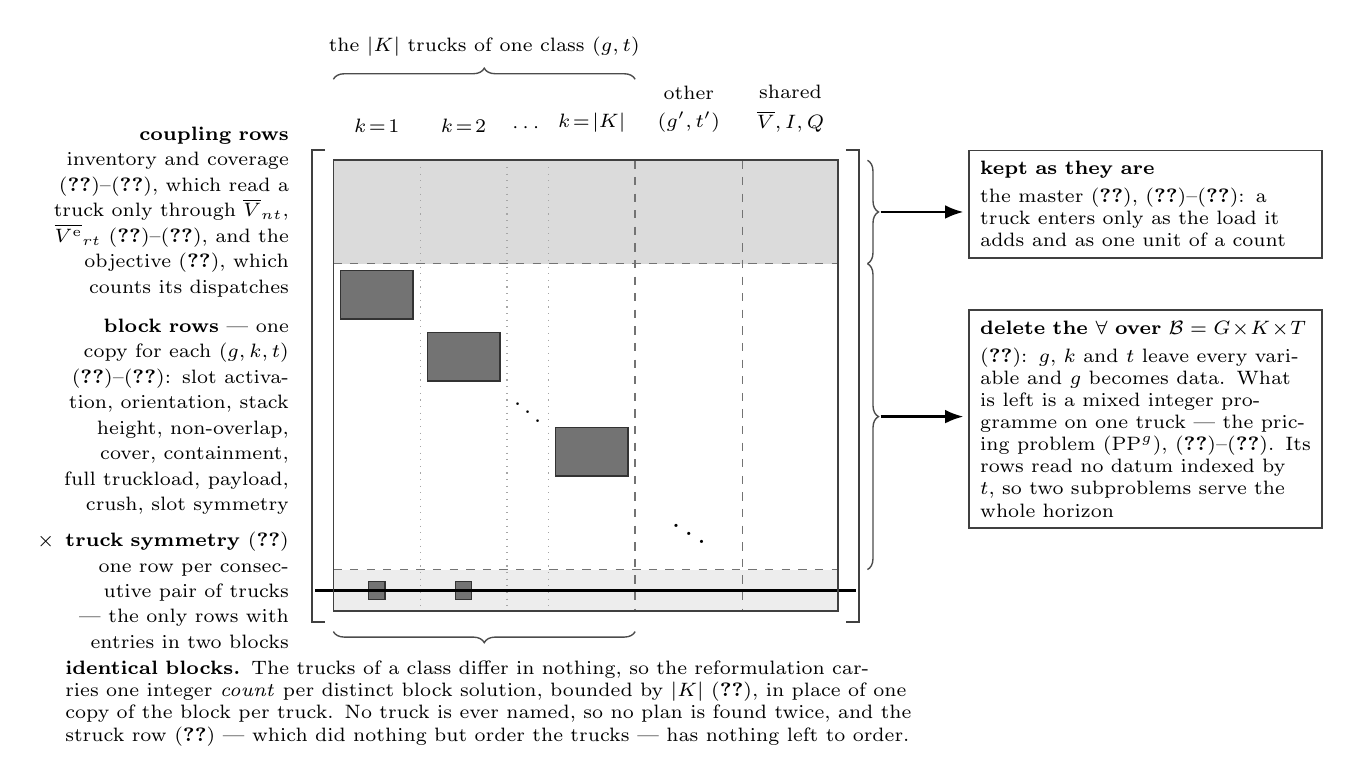
\begin{tikzpicture}[>=Latex, x=1.05cm, y=1.05cm,
  cpl/.style={fill=black!14, draw=none},
  blk/.style={fill=black!55, draw=black!80, line width=0.5pt},
  sep/.style={draw=black!35, dotted, line width=0.4pt},
  cls/.style={draw=black!55, dashed, line width=0.5pt},
  brc/.style={decorate, black!70, line width=0.5pt},
  box/.style={draw=black!75, fill=white, line width=0.6pt, inner sep=4pt,
              align=left, font=\scriptsize, text width=42mm,
              execute at begin node=\blknohyph},
  rl/.style={font=\scriptsize\linespread{1.15}\selectfont, align=right,
             text width=32mm, anchor=east, execute at begin node=\blknohyph},
  hd/.style={font=\scriptsize, align=center, anchor=south},
  nt/.style={font=\scriptsize, align=left, execute at begin node=\blknohyph}]

  % ---- column boundaries (x) and row boundaries (y) ---------------------
  \def\xa{0}    \def\xb{1.05} \def\xc{2.10} \def\xd{2.60}
  \def\xe{3.65} \def\xf{4.95} \def\xg{6.10}
  \def\ya{0}    \def\yb{-1.25}
  \def\yc{-2.00}\def\yd{-2.75}\def\ye{-3.15}\def\yf{-3.90}\def\yg{-4.95}
  \def\yh{-5.45}

  % ---- the coupling band, with entries in every column ------------------
  \fill[cpl] (\xa,\ya) rectangle (\xg,\yb);

  % ---- the diagonal: one block per (g,k,t), nothing off it --------------
  \fill[blk] (0.085,-1.33) rectangle (0.965,-1.92);
  \fill[blk] (1.135,-2.08) rectangle (2.015,-2.67);
  \fill[blk] (2.685,-3.23) rectangle (3.565,-3.82);
  \node[font=\small] at (2.35,-2.95) {$\ddots$};
  \node[font=\large] at (4.30,-4.42) {$\ddots$};

  % ---- the one row that is not block-diagonal, struck out ---------------
  \fill[black!7]  (\xa,\yg)    rectangle (\xg,\yh);
  \fill[black!55, draw=black!80, line width=0.4pt]
     (0.425,-5.09) rectangle (0.625,-5.31);
  \fill[black!55, draw=black!80, line width=0.4pt]
     (1.475,-5.09) rectangle (1.675,-5.31);
  \draw[black, line width=1.1pt] (-0.22,-5.20) -- (6.32,-5.20);

  % ---- grid: column groups, and the two row bands -----------------------
  \foreach \x in {\xb,\xc,\xd} \draw[sep] (\x,\ya) -- (\x,\yh);
  \draw[cls] (\xe,\ya) -- (\xe,\yh);
  \draw[cls] (\xf,\ya) -- (\xf,\yh);
  \draw[cls] (\xa,\yb) -- (\xg,\yb);
  \draw[cls] (\xa,\yg) -- (\xg,\yg);
  \draw[black!75, line width=0.6pt] (\xa,\ya) rectangle (\xg,\yh);
  \draw[black!75, line width=0.7pt]
     (-0.10,0.13) -- (-0.26,0.13) -- (-0.26,-5.58) -- (-0.10,-5.58);
  \draw[black!75, line width=0.7pt]
     (6.20,0.13) -- (6.36,0.13) -- (6.36,-5.58) -- (6.20,-5.58);

  % ---- column headers ---------------------------------------------------
  \node[hd] at (0.525,0.22) {$k\!=\!1$};
  \node[hd] at (1.575,0.22) {$k\!=\!2$};
  \node[hd] at (2.350,0.22) {$\cdots$};
  \node[hd] at (3.125,0.22) {$k\!=\!|K|$};
  \node[hd, text width=13mm] at (4.30,0.22) {other\\[2pt]$(g',t')$};
  \node[hd, text width=12mm] at (5.53,0.22) {shared\\[3pt]$\overline{V},I,Q$};
  \draw[brc, decoration={brace, amplitude=4pt}] (\xa,0.98) -- (\xe,0.98);
  \node[font=\scriptsize, anchor=south] at (1.825,1.14)
     {the $|K|$ trucks of one class $(g,t)$};

  % ---- row labels -------------------------------------------------------
  \node[rl] at (-0.42,-0.625)
     {\textbf{coupling rows}\\ inventory and coverage
      \eqref{sb:eq:inv-plant-main}--\eqref{sb:eq:safety-empty}, which read a
      truck only through $\overline{V}_{nt}$, $\overline{V^{\mathrm{e}}}_{rt}$
      \eqref{sb:eq:agg-V}--\eqref{sb:eq:agg-Ve}, and the objective
      \eqref{sb:eq:obj}, which counts its dispatches};
  \node[rl] at (-0.42,-3.10)
     {\textbf{block rows} --- one copy for each $(g,k,t)$\\
      \eqref{sb:eq:slot-active}--\eqref{sb:eq:sym}: slot activation,
      orientation, stack height, non-overlap, cover, containment,
      full truckload, payload, crush, slot symmetry};
  \node[rl] at (-0.42,-5.20)
     {$\times$\, \textbf{truck symmetry} \eqref{dec:sym-truck}\\
      one row per consecutive pair of trucks --- the only rows with entries
      in two blocks};

  % ---- what each band becomes ------------------------------------------
  \draw[brc, decoration={brace, mirror, amplitude=4pt}] (6.46,\yb) -- (6.46,\ya);
  \draw[->, line width=0.8pt] (6.62,-0.625) -- (7.62,-0.625);
  \node[box, anchor=north west] at (7.68,0.13)
     {\textbf{kept as they are}\\[2pt]
      the master \eqref{eq:MPObjective},
      \eqref{bp:MP-def-V}--\eqref{bp:MP-count}: a truck enters only as the
      load it adds and as one unit of a count};

  \draw[brc, decoration={brace, mirror, amplitude=4pt}] (6.46,\yg) -- (6.46,\yb);
  \draw[->, line width=0.8pt] (6.62,-3.10) -- (7.62,-3.10);
  \node[box, anchor=north west] at (7.68,-1.80)
     {\textbf{delete the $\forall$ over
      $\mathcal{B}=G\!\times\!K\!\times\!T$}\\[2pt]
      \eqref{eq:deletequant}: $g$, $k$ and $t$ leave every variable and $g$
      becomes data. What is left
      is a mixed integer programme on one truck --- the pricing problem
      $(\mathrm{PP}^{g})$, \eqref{bp:PP-objective}--\eqref{bp:PP-utilw}. Its
      rows read no datum indexed by $t$, so two subproblems serve the whole
      horizon};

  % ---- the aggregation, under the diagonal ------------------------------
  \draw[brc, decoration={brace, mirror, amplitude=4pt}] (\xa,-5.70) -- (\xe,-5.70);
  \node[nt, anchor=north, text width=108mm] at (1.90,-5.94)
     {\textbf{identical blocks.} The trucks of a class differ in nothing, so
      the reformulation carries one integer \emph{count} per distinct block
      solution, bounded by $|K|$ \eqref{bp:MP-count}, in place of one copy of
      the block per truck. No truck is ever named, so no plan is found twice,
      and the struck row \eqref{dec:sym-truck} --- which did nothing but order
      the trucks --- has nothing left to order.};

\end{tikzpicture}}
\caption{The decomposition is read off the formulation, not chosen by
analogy. Every geometric, stacking, crush, payload and full-truckload
row of Section~\ref{sec:model} is confined to one truck, so the matrix
is block-angular over $\mathcal{B}=G\times K\times T$; deleting the
quantifier over $\mathcal{B}$ from those rows leaves a mixed integer
programme on a single truck, and that programme is the pricing
problem. Nothing is invented for the subproblem and no geometry stays
behind in the master, which is why a branching row added to the master
never changes what the subproblem is.
Table~\ref{tab:rowmap} is the same statement row by row.}
\label{fig:blocks}
\end{figure}


\paragraph{Blocks.}
Take the block index to be $\mathcal{B}=G\times K\times T$. Every row
from \eqref{sb:eq:slot-active} to \eqref{dec:sym-truck} --- the first
column of Table~\ref{tab:rowmap} names them --- carries a single
direction, truck and period as a fixed $\forall$ index or a literal,
and none couples two values of $g$, $k$ or $t$; the exception is
\eqref{dec:sym-truck}, relating truck $k+1$ to truck $k$. The remaining
rows are the objective, the inventory and coverage block
\eqref{sb:eq:inv-plant-main}--\eqref{sb:eq:safety-empty} and the two
definitions \eqref{sb:eq:agg-V}--\eqref{sb:eq:agg-Ve}, and they see
the blocks \emph{only} through those aggregates and the count of
dispatches $z^{K}$ charges for. Block-angularity over $\mathcal{B}$ is
therefore a property of the formulation, not a discovery about it.

\paragraph{Delete the quantifier.}
Fix a class $(g,t)$, take the block rows, and \emph{remove the
$\forall$ over $\mathcal{B}$}: drop the indices $g$, $k$ and $t$ from
every variable and read $g$ as data. The stack-height row, for
instance, goes
\begin{equation}
\underbrace{\sum_{r\in R(h)} r_{gr}L_{gihktr}\le rK\,X_{gihkt}
  \quad\forall g,h,i,k,t}_{\text{3D-SCPTOP, }\eqref{sb:eq:height}}
\;\longmapsto\;
\underbrace{\sum_{r\in R(h)} r_{gr}L_{ihr}\le rK\,X_{ih}
  \quad\forall h,i}_{(\mathrm{PP}^{g}),\ \eqref{bp:PP-height}},
\label{eq:deletequant}
\end{equation}
and every other block row the same way; what is left is a mixed integer
programme over one truck, the $(\mathrm{PP}^{g})$ of
Section~\ref{sec:pricing}. Nothing is invented for the subproblem and
nothing of the geometry is left behind in the master. Two rows do not
make the journey: \eqref{dec:sym-truck}, which the aggregation
disposes of, and \eqref{sb:eq:lc-active}, whose two binaries collapse
into one (Section~\ref{sec:pricing}).


\paragraph{Identical blocks.}
$K$ is anonymous, so the blocks of a fixed $(g,t)$ are identical and
are aggregated: in place of one copy per truck, the reformulation
carries one non-negative integer variable per block \emph{solution},
counting how many of the class's blocks take it, and one row per class
bounding that count by $|K|$. This is where the second difficulty
disappears --- the trucks are never distinguished, so there is no
permutation to search --- and it is why the dropped row costs nothing:
counts carry no order, so the master has no variable in which to
express \eqref{dec:sym-truck}. The converse direction of
Proposition~\ref{prop:equiv} assigns trucks \emph{in index order}, so
the equivalence holds against the compact model \emph{with} that row in
force.

\paragraph{Classes.}
The classes are the pairs $(g,t)$, and within a class the block rows
are pinned to the class's $g$, so there is one pricing problem per
\emph{direction}. The pricing rows read no datum indexed by $t$ --- the
trailer, the stack types, the crush limit and the floor are
time-invariant --- so the periods of one direction differ \emph{only in
their duals}, one column set serves them all, and the whole horizon
costs two pricing problems rather than $2|T|$.

\paragraph{Discretisation.}
Every block variable that reaches the master is integer, so a block
solution may be taken to be an \emph{integer} point of its pricing
problem completed by placement coordinates. The multipliers are then
integer rather than merely non-negative, and a fractional one is a
genuine integrality violation.

\begin{longtable}[hbt!]{@{}p{0.30\textwidth}p{0.30\textwidth}p{0.34\textwidth}@{}}
\caption{The block rows of Section~\ref{sec:model} and the rows of
$(\mathrm{PP}^{g})$ they become when the $\forall$ over
$\mathcal{B}=G\times K\times T$ is deleted. The two directions share
the geometry, so it is written once with $g$ as data; the
direction-specific rows are those of Section~\ref{sec:pp-dir}. One row
of $(\mathrm{PP}^{g})$ is not a transcription and is marked as such.}
\label{tab:rowmap}\\
\toprule
Row & Section~\ref{sec:model} & $(\mathrm{PP}^{g})$ \\
\midrule
\endfirsthead
\toprule
Row & Section~\ref{sec:model} & $(\mathrm{PP}^{g})$ \\
\midrule
\endhead
\multicolumn{3}{@{}l}{\textit{Block rows: the pricing problem}}\\
Slot active            & \eqref{sb:eq:slot-active} & \eqref{bp:PP-slot-active}\\
Orientation            & \eqref{sb:eq:orient}      & \eqref{bp:PP-orient}\\
Stack height           & \eqref{sb:eq:height}      & \eqref{bp:PP-height}\\
Non-overlap            & \eqref{sb:eq:nonov-x1}--\eqref{sb:eq:nonov-y2} & \eqref{bp:PP-nonov-x1}--\eqref{bp:PP-nonov-y2}\\
Cover                  & \eqref{sb:eq:cover}       & \eqref{bp:PP-cover}\\
Containment            & \eqref{sb:eq:cont-x}--\eqref{sb:eq:cont-y} & \eqref{bp:PP-cont-x}\\
Full truckload, volume & \eqref{sb:eq:util-p}, \eqref{sb:eq:util-s} & \eqref{bp:PP-util}\\
Full truckload, payload& \eqref{sb:eq:utilw-p}, \eqref{sb:eq:utilw-s} & \eqref{bp:PP-utilw}\\
The same on capacity   & \eqref{sb:eq:util-cap} & \eqref{bp:PP-cap}, re-gated on $Z$\\
Occupied floor area    & --- (no counterpart)      & \eqref{bp:PP-areacut}, a valid inequality\\
Slot capacity          & \eqref{sb:eq:slot-cap}    & \eqref{bp:PP-p-slot-cap}\\
Folded capacity        & \eqref{sb:eq:empty-cap}   & \eqref{bp:PP-s-empty-cap}\\
Dispatch gate, full    & \eqref{fix:slot-link}     & \eqref{bp:PP-p-slot-link}\\
Dispatch gate, folded  & \eqref{fix:empty-link}    & \eqref{bp:PP-s-empty-link}\\
Payload, both directions & \eqref{sb:eq:truck-w-plant} & \eqref{bp:PP-p-truck-w}, \eqref{bp:PP-s-truck-w}\\
Crush limit, plant-bound & \eqref{sb:eq:stack-w-plant} & \eqref{bp:PP-p-stack-w}\\
Crush limit, supplier-bound & \eqref{sb:eq:stack-w-sup} & \eqref{bp:PP-s-stack-w}\\
Slot symmetry          & \eqref{sb:eq:sym}         & \eqref{bp:PP-sym}\\
Transport cost         & \eqref{sb:eq:obj-zK}      & $\eta^{K}cK\cdot Z$ in \eqref{bp:PP-objective}\\
Dispatch               & \eqref{sb:eq:lc-active}   & deleted; $Z$ carries the truck\\
Truck symmetry         & \eqref{dec:sym-truck}     & dropped in the aggregation\\
\midrule
\multicolumn{3}{@{}l}{\textit{Coupling rows: the master}}\\
Aggregate flows        & \eqref{sb:eq:agg-V}--\eqref{sb:eq:agg-Ve} & \eqref{bp:MP-def-V}--\eqref{bp:MP-def-Ve}\\
Fleet per class        & $|K|$ trucks per $(g,t)$  & \eqref{bp:MP-count}\\
Inventory and coverage & \eqref{sb:eq:inv-plant-main}--\eqref{sb:eq:safety-empty} & verbatim in the master\\
Holding cost           & \eqref{sb:eq:obj-zK}      & second term of \eqref{eq:MPObjective}\\
\bottomrule
\end{longtable}


\FloatBarrier

\section{The master problem}
\label{sec:master}

\subsection{Columns}
\label{sec:columns}

A column of a direction is the image of a feasible point of that
direction's pricing problem, together with the point itself as a
witness; $\Omega^{p}$ and $\Omega^{s}$ are the two column sets, indexed
by $\omega$. A \emph{plant-bound} column $\omega\in\Omega^{p}$ is a
vector $b_{\omega}=(b_{\omega n})_{n\in N}$ of full RTIs --- the value
of $\overline{V}_{n}$ at the point --- for which there exist a slot
count $m\le|I|$, stack types $h_{1},\dots,h_{m}\in H$, orientations,
bottom-left coordinates $(x_{i},y_{i})$, layer counts $\ell_{ir}$ and
per-slot product loads $v_{in}$ such that
\begin{align}
&\text{the $m$ footprints, rotated as chosen, do not overlap and lie
   inside } pK\times qK,
   \label{eq:col-geom}\\
&\textstyle\sum_{r\in R(h_{i})} r_{pr}\ell_{ir}\;\le\;rK
   &&\forall i\le m,
   \label{eq:col-height}\\
&\textstyle\sum_{n\in M(r)} v_{in}\;\le\;n_{h_{i}r}\ell_{ir}
   &&\forall i\le m,\;r\in R,
   \label{eq:col-assign}\\
&\textstyle\sum_{n\in N} w_{n}v_{in}\;\le\;W^{\max}
   &&\forall i\le m,
   \label{eq:col-crush}\\
&\textstyle\sum_{n\in N} w_{n}b_{\omega n}\;\le\;pK^{w},
   \qquad
   \max\Bigl\{\tfrac{\sum_{n}\gamma_{p\rho(n)}b_{\omega n}}{\Gamma_{K}},\;
              \tfrac{\sum_{n}w_{n}b_{\omega n}}{pK^{w}}\Bigr\}\;\ge\;\alpha,
   \label{eq:col-truck}\\
&b_{\omega n}=\textstyle\sum_{i\le m} v_{in}
   &&\forall n\in N.
   \label{eq:col-agg}
\end{align}
These are the block rows of Section~\ref{sec:model} read on one truck
(Table~\ref{tab:rowmap}); in \eqref{eq:col-assign} $n_{h_{i}r}\ell_{ir}$
is read as $0$ for $r\notin R(h_{i})$, and it is an \emph{inequality}
because a partly filled layer is a legal compact layout.

A \emph{supplier-bound} column is the analogous object
$e_{\omega}=(e_{\omega r})_{r\in R}$ over folded heights, weights and
volumes, with \eqref{sb:eq:stack-w-sup} as its per-slot crush condition
and $e_{\omega r}\le\sum_{i\le m}n_{h_{i}r}\ell_{ir}$, which is
\eqref{sb:eq:empty-cap}, in place of \eqref{eq:col-assign} and
\eqref{eq:col-agg}; the weight of a folded RTI depends only on its
type, so no product assignment is needed. We write
\eqref{eq:col-geom}--\eqref{eq:col-agg} from here on for either
direction, writing $\mathrm{image}_{c}(\omega)$ for the entry of
$b_{\omega}$ or $e_{\omega}$ at the \emph{commodity} $c$ --- a
product when $g=\mathrm{p}$, an RTI type when $g=\mathrm{s}$. Every column costs $c_{\omega}=\eta^{K}cK$, and
$\Omega^{g}$ holds the \emph{non-empty} columns only, the all-zero
point being the slack of \eqref{bp:MP-count}.

Two features of this definition carry the method: the column holds the
per-slot assignment $v_{in}$, so \eqref{eq:col-crush} is the
period-exact cap \eqref{sb:eq:stack-w-plant} and not the family
surrogate a catalogue of capacity-only configurations must use, and it
retains its witnessing placement, so a plan is a set of drawings.

\subsection{The master}
\label{sec:mp}

Let $\lambda^{g}_{\omega t}\in\mathbb{Z}_{\ge0}$ be the number of
trucks of class $(g,t)$ dispatched carrying column $\omega$. The master
problem (MP) is
\begin{align}
  \min\;\; & \sum_{g\in G}\sum_{t\in T}\sum_{\omega\in \Omega^{g}}
                c_{\omega}\,\lambda^{g}_{\omega t}
    \;+\;\eta^{I}\sum_{g\in G}\sum_{n\in N}\sum_{t\in T} ic_{gn} I_{gnt}
    \label{eq:MPObjective}
\end{align}
subject to
\begin{align}
  \overline{V}_{nt}
    &= \sum_{\omega\in \Omega^{p}} b_{\omega n}\,\lambda^{p}_{\omega t}
    &&\forall n\in N,\;t\in T \label{bp:MP-def-V}\\
  \overline{V^{\mathrm{e}}}_{rt}
    &= \sum_{\omega\in \Omega^{s}} e_{\omega r}\,\lambda^{s}_{\omega t}
    &&\forall r\in R,\;t\in T \label{bp:MP-def-Ve}\\
  \sum_{\omega\in \Omega^{g}} \lambda^{g}_{\omega t} &\le |K|
    &&\forall g\in G,\;t\in T \label{bp:MP-count}\\
  &\text{\eqref{sb:eq:inv-plant-main}--\eqref{sb:eq:safety-empty}}
    &&\text{verbatim} \nonumber\\
  \lambda^{g}_{\omega t}&\in\mathbb{Z}_{\ge0},\quad
  I_{gnt},\,Ie_{gtr}\in\mathbb{Z}_{\ge0},\quad
  \overline{V}_{nt},\,\overline{V^{\mathrm{e}}}_{rt}\in\mathbb{Z}_{\ge0}
  \ \text{(implied by \eqref{bp:MP-def-V}--\eqref{bp:MP-def-Ve})}.
    \nonumber
\end{align}
That is the whole master: every column costs the same, so the transport
term is $cK$ times the number dispatched, and
\eqref{bp:MP-def-V}--\eqref{bp:MP-def-Ve} are
\eqref{sb:eq:agg-V}--\eqref{sb:eq:agg-Ve} with each truck's load
replaced by its column's image. Since $\Omega^{g}$ holds the non-empty
columns only, $\overline{\lambda}_{gt}=\sum_{\omega}\lambda^{g}_{\omega
t}$ is the number \emph{dispatched} by class $(g,t)$, which is what
Section~\ref{sec:branching} branches on.

\begin{proposition}[equivalence]
\label{prop:equiv}
MP and 3D-SCPTOP have the same optimal value.
\end{proposition}
\begin{proof}
Each used truck $(g,k,t)$ of a 3D-SCPTOP solution induces a load vector
satisfying its direction's column conditions, read off its own layout
with $\ell_{ir}=L_{g,i,h_{i},k,t,r}$ and, at the plant,
$v_{in}=V_{kint}$; every one of those conditions is a row the truck
already satisfies. Counting trucks by load vector gives a feasible MP
solution of equal cost, since transport cost depends only on the number
of used trucks and the inventory rows see only the aggregates
\eqref{bp:MP-def-V}--\eqref{bp:MP-def-Ve} reproduce. Conversely, give
each truck of an MP solution the layout witnessing its column: the
blocks are identical, so any assignment serves, and in index order the
result also satisfies \eqref{dec:sym-truck}.
\end{proof}

\noindent No hypothesis is needed because there is no catalogue of
layouts to be sized: in Section~\ref{sec:model} a truck's layout is
its own. MP is therefore the same problem written differently, and any
bound derived from it bounds the original.

\subsection{The restricted master and the reduced cost}
\label{sec:rmp}

$|\Omega^{g}|$ is astronomical, so MP is solved over a subset
$\bar\Omega^{g}$ with integrality relaxed --- the restricted master
problem (RMP) --- whose duals the pricing problems use to look for
columns of negative reduced cost (Figure~\ref{fig:loop}). With
$\pi_{nt},\pi_{rt}$ the duals of
\eqref{bp:MP-def-V}--\eqref{bp:MP-def-Ve} and $\mu_{gt}\le0$ that of
\eqref{bp:MP-count}, the reduced cost of a plant-bound column
dispatched in $t$ is
\begin{equation}
\bar c(\omega,t)\;=\;c_{\omega}-\sum_{n\in N}\pi_{nt}\,b_{\omega n}
                              -\mu_{pt},
\label{eq:redcost}
\end{equation}
and analogously at the supplier. The pricing problem of class $(g,t)$
minimises $c(x)-\sum_{c}\pi_{ct}\,\mathrm{image}_{c}(x)$ over the
feasible points of the direction's block, so with optimal value
$z^{\star}_{gt}$ it gives
$\min_{\omega}\bar c(\omega,t)=z^{\star}_{gt}-\mu_{gt}$, and a column
enters when that is negative.

% The master problem (step 2), drawn as the incidence pattern of its rows:
% what a column writes into, what the artificials sit on, and -- the point --
% the row family that is not there.  The generation loop survives as the two
% margin arrows: columns enter top left, duals leave top right.
% Uses only tikz with calc/positioning/arrows.meta, all loaded by
% ../necessarypackages.  Drawn at final size (<= 15.1 cm against a 15.24 cm
% \textwidth): no \resizebox, so \scriptsize stays \scriptsize on the page.
% Every qualifier lives in the row label, never in a cell, so no cell can
% outgrow its row; the row heights below are set to the label line counts,
% and the column heads are at most three lines so they clear the head rule.
\begin{figure}[htb]
\centering
\hbadness=10000
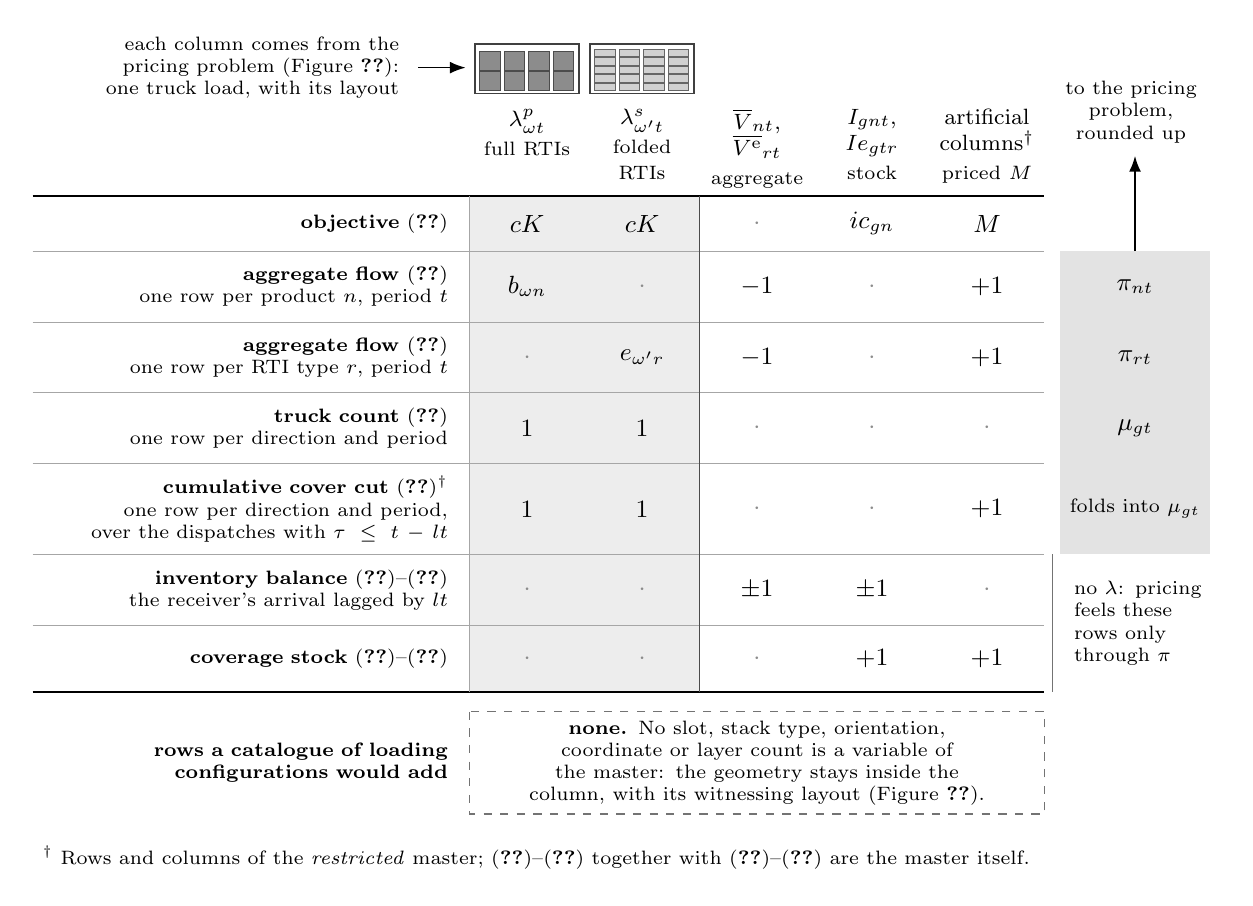
\begin{tikzpicture}[x=1cm, y=1cm, >=Latex, line width=0.5pt,
  rl/.style  ={font=\scriptsize, align=right, text width=52mm, anchor=east},
  ce/.style  ={font=\small,      align=center},
  hd/.style  ={font=\footnotesize, align=center, text width=14mm,
               anchor=north, inner sep=1pt},
  nt/.style  ={font=\scriptsize, align=center, text width=18mm},
  dot/.style ={font=\small, color=black!45}]

% ---------------------------------------------------------------- geometry
\def\xS{5.55}\def\xB{12.85}                 % body left / right edge
\def\xa{6.28}\def\xb{7.74}\def\xc{9.20}\def\xd{10.66}\def\xe{12.12}
\def\xD{13.05}\def\xE{14.95}                % the dual strip
\def\yH{-2.25}
\def\yA{-2.95}\def\yB{-3.85}\def\yC{-4.75}\def\yD{-5.65}\def\yE{-6.80}
\def\yF{-7.70}\def\yG{-8.55}

% ------------------------------------------------------- shading and rules
\fill[black!7]  (\xS,\yH) rectangle (8.47,\yG);          % the column block
\fill[black!11] (\xD,\yA) rectangle (\xE,\yE);           % what pricing gets
\draw[line width=0.8pt] (0,\yH) -- (\xB,\yH);
\draw[line width=0.8pt] (0,\yG) -- (\xB,\yG);
\foreach \y in {\yA,\yB,\yC,\yD,\yE,\yF}
   \draw[black!35, line width=0.3pt] (0,\y) -- (\xB,\y);
\draw[black!35, line width=0.3pt] (\xS,\yH) -- (\xS,\yG);
\draw[black!70, line width=0.6pt] (8.47,\yH) -- (8.47,\yG);

% ------------------------------------------------------ the two pictograms
% a plant-bound load: stacks of full RTIs; a supplier-bound load: the same
% floor carrying folded ones.  That is the whole difference between the two
% directions as far as the master is concerned.
\draw[black!75, fill=white, line width=0.6pt]
   (\xa-0.66,-0.95) rectangle (\xa+0.66,-0.32);
\foreach \i in {0,1,2,3}{\foreach \j in {0,1}{
   \draw[black!70, fill=black!45, line width=0.3pt]
      (\xa-0.60+\i*0.31,-0.91+\j*0.255) rectangle ++(0.26,0.24);}}
\draw[black!75, fill=white, line width=0.6pt]
   (\xb-0.66,-0.95) rectangle (\xb+0.66,-0.32);
\foreach \i in {0,1,2,3}{\foreach \j in {0,1,2,3,4}{
   \draw[black!60, fill=black!18, line width=0.3pt]
      (\xb-0.60+\i*0.31,-0.91+\j*0.108) rectangle ++(0.26,0.09);}}

% --------------------------------------------- columns in, duals out (loop)
\node[rl, text width=46mm] at (4.78,-0.62)
   {each column comes from the pricing problem
    (Figure~\ref{fig:truck}): one truck load, with its layout};
\draw[->, line width=0.6pt] (4.90,-0.62) -- (5.50,-0.62);

\draw[->, line width=0.6pt] (14.00,\yA) -- (14.00,-1.74);
\node[nt, text width=21mm, anchor=south] at (13.95,-1.70)
   {to the pricing problem, rounded up};

% ------------------------------------------------------------ column heads
\node[hd] at (\xa,-1.10) {$\lambda^{p}_{\omega t}$\\[1pt]
   {\scriptsize full RTIs}};
\node[hd] at (\xb,-1.10) {$\lambda^{s}_{\omega' t}$\\[1pt]
   {\scriptsize folded RTIs}};
\node[hd] at (\xc,-1.10) {$\overline{V}_{nt}$,\\ $\overline{V^{\mathrm{e}}}_{rt}$\\[1pt]
   {\scriptsize aggregate}};
\node[hd] at (\xd,-1.10) {$I_{gnt}$,\\ $Ie_{gtr}$\\[1pt]
   {\scriptsize stock}};
\node[hd] at (\xe,-1.10) {artificial\\ columns$^{\dagger}$\\[1pt]
   {\scriptsize priced $M$}};

% ------------------------------------------------------------- row 1: cost
\node[rl] at (5.40,-2.60) {\textbf{objective} \eqref{eq:MPObjective}};
\node[ce]  at (\xa,-2.60) {$cK$};
\node[ce]  at (\xb,-2.60) {$cK$};
\node[dot] at (\xc,-2.60) {$\cdot$};
\node[ce]  at (\xd,-2.60) {$ic_{gn}$};
\node[ce]  at (\xe,-2.60) {$M$};

% ------------------------------------------ rows 2-3: the only link to load
\node[rl] at (5.40,-3.40) {\textbf{aggregate flow} \eqref{bp:MP-def-V}\\
   one row per product $n$, period $t$};
\node[ce]  at (\xa,-3.40) {$b_{\omega n}$};
\node[dot] at (\xb,-3.40) {$\cdot$};
\node[ce]  at (\xc,-3.40) {$-1$};
\node[dot] at (\xd,-3.40) {$\cdot$};
\node[ce]  at (\xe,-3.40) {$+1$};
\node[ce]  at (14.00,-3.40) {$\pi_{nt}$};

\node[rl] at (5.40,-4.30) {\textbf{aggregate flow} \eqref{bp:MP-def-Ve}\\
   one row per RTI type $r$, period $t$};
\node[dot] at (\xa,-4.30) {$\cdot$};
\node[ce]  at (\xb,-4.30) {$e_{\omega' r}$};
\node[ce]  at (\xc,-4.30) {$-1$};
\node[dot] at (\xd,-4.30) {$\cdot$};
\node[ce]  at (\xe,-4.30) {$+1$};
\node[ce]  at (14.00,-4.30) {$\pi_{rt}$};

% ------------------------------------------------------- row 4: truck count
\node[rl] at (5.40,-5.20) {\textbf{truck count} \eqref{bp:MP-count}\\
   one row per direction and period};
\node[ce]  at (\xa,-5.20) {$1$};
\node[ce]  at (\xb,-5.20) {$1$};
\node[dot] at (\xc,-5.20) {$\cdot$};
\node[dot] at (\xd,-5.20) {$\cdot$};
\node[dot] at (\xe,-5.20) {$\cdot$};
\node[ce]  at (14.00,-5.20) {$\mu_{gt}$};

% -------------------------------------------------------- row 5: cover cuts
\node[rl] at (5.40,-6.225) {\textbf{cumulative cover cut}
   \eqref{eq:covercut}$^{\dagger}$\\
   one row per direction and period, over the dispatches with $\tau\le t-lt$};
\node[ce]  at (\xa,-6.225) {$1$};
\node[ce]  at (\xb,-6.225) {$1$};
\node[dot] at (\xc,-6.225) {$\cdot$};
\node[dot] at (\xd,-6.225) {$\cdot$};
\node[ce]  at (\xe,-6.225) {$+1$};
\node[nt]  at (14.00,-6.225) {folds into $\mu_{gt}$};

% -------------------------------------------- rows 6-7: inventory, coverage
\node[rl] at (5.40,-7.25) {\textbf{inventory balance}
   \eqref{sb:eq:inv-plant-main}--\eqref{sb:eq:inve-sup-init}\\
   the receiver's arrival lagged by $lt$};
\node[dot] at (\xa,-7.25) {$\cdot$};
\node[dot] at (\xb,-7.25) {$\cdot$};
\node[ce]  at (\xc,-7.25) {$\pm1$};
\node[ce]  at (\xd,-7.25) {$\pm1$};
\node[dot] at (\xe,-7.25) {$\cdot$};

\node[rl] at (5.40,-8.125) {\textbf{coverage stock}
   \eqref{sb:eq:safety-full}--\eqref{sb:eq:safety-empty}};
\node[dot] at (\xa,-8.125) {$\cdot$};
\node[dot] at (\xb,-8.125) {$\cdot$};
\node[dot] at (\xc,-8.125) {$\cdot$};
\node[ce]  at (\xd,-8.125) {$+1$};
\node[ce]  at (\xe,-8.125) {$+1$};

\draw[black!55, line width=0.4pt] (12.95,\yE) -- (12.95,\yG);
\node[nt, text width=18mm, align=left, anchor=west] at (13.10,-7.675)
   {no $\lambda$: pricing feels these rows only through $\pi$};

% ------------------------------------------------- the rows that are absent
\node[rl] at (5.40,-9.45) {\textbf{rows a catalogue of loading\\
   configurations would add}};
\draw[dashed, black!55, line width=0.5pt] (\xS,-8.80) rectangle (\xB,-10.10);
\node[font=\scriptsize, align=center, text width=68mm] at (9.20,-9.45)
   {\textbf{none.} No slot, stack type, orientation, \mbox{coordinate} or
    layer count is a variable of the master: the geometry stays inside the
    \mbox{column}, with its witnessing layout (Figure~\ref{fig:truck}).};

% ----------------------------------------------------------------- the note
\node[font=\scriptsize, align=left, text width=149mm, anchor=north west]
   at (0,-10.38)
   {$^{\dagger}$ Rows and columns of the \emph{restricted} master;
    \eqref{eq:MPObjective}--\eqref{bp:MP-count} together with
    \eqref{sb:eq:inv-plant-main}--\eqref{sb:eq:safety-empty} are the master
    itself.};

\end{tikzpicture}
\caption{The master is a flow model that has never seen a box. A column is
one truck load, and the only rows it enters are the two aggregate-flow
definitions, one truck count per direction and period, and the cumulative
cover cut --- every one of which merely counts or sums what the load
contains. No slot, stack type, orientation, coordinate or layer count is a
variable here, so there is no catalogue of loading configurations to
enumerate, and no row written over these variables can reach the geometry;
the inventory and coverage rows see the trucks only through $\overline{V}$
and $\overline{V^{\mathrm{e}}}$, and all that ever reaches the pricing
problem is $\pi$ and $\mu$. The non-negative artificials keep the restricted
master feasible, and its duals defined, for any pool --- a solution that uses
them is not a plan.}
\label{fig:loop}
\end{figure}


The prices, irrational in general, must be rounded \emph{upwards}
before entering an integer-coefficient subproblem, never to nearest, so
that the rounded objective dominates the true one and the subproblem's
value stays an over-estimate of the true maximum, as the certificate
below requires. Rounding to nearest invalidates that certificate and,
with reduced costs near zero, returns a value just above the threshold
so that convergence is never declared.

The RMP is \emph{elastic}: non-negative artificials sit on
\eqref{bp:MP-def-V}--\eqref{bp:MP-def-Ve}, on the coverage rows and on
the cuts below at a large price, so it is feasible for any pool and
always yields duals, and a solution with positive artificials is not a
plan. The elasticity is one-sided where it matters: a definition row
reads $\overline{V}=\sum_{\omega}b\lambda+\text{art}$,
$\text{art}\ge0$, so slack can only enlarge a delivery --- which is
why stock non-negativity stays rigid against a fleet lower bound.

It also carries cumulative cover cuts. With $\rho^{g}_{ct}$ the
cumulative requirement of commodity $c$ at the receiving node $g$
through $t$ --- demand to date plus the coverage stock of $t$, net of
initial stock and freight in transit, floored at zero --- and
$\bar u^{g}=\min\{\lfloor pK^{w}/\min_{c}w_{c}\rfloor,\,
\lfloor\Gamma_{K}/\min_{c}\gamma_{gc}\rfloor\}$ an upper bound on the
units one truck holds, every $t>lt$ gives
\begin{equation}
\sum_{\tau\le t-lt}\ \sum_{\omega\in\Omega^{g}}\lambda^{g}_{\omega\tau}
\;\ge\;
\max\Bigl\{\Bigl\lceil\tfrac{\sum_{c}\gamma_{gc}\rho^{g}_{ct}}{\Gamma_{K}}\Bigr\rceil,\;
\Bigl\lceil\tfrac{\sum_{c}w_{c}\rho^{g}_{ct}}{pK^{w}}\Bigr\rceil,\;
\Bigl\lceil\tfrac{\sum_{c}\rho^{g}_{ct}}{\bar u^{g}}\Bigr\rceil\Bigr\}.
\label{eq:covercut}
\end{equation}
Each ratio divides a requirement by the most one truck can carry of
that resource, so over-estimating $\bar u^{g}$ only weakens the cut
while the shift by $lt$ is mandatory. Its duals fold into $\mu_{gt}$
and leave \eqref{eq:redcost} exact, which is possible exactly when a
row $\sum_{\omega}\phi(\omega)\lambda_{\omega}\lessgtr\beta$ has $\phi$
constant within a class or affine in the column's image. Such a row is
\emph{robust}: it changes the duals and nothing else. Every row this
paper adds is of that kind, which is why no branching decision reaches
a pricing problem.

Finally the RMP is \emph{period-scoped}: a column priced at $t$
receives a dispatch variable at $t$ alone. That changes the restricted
master's size and not the master's, so a sweep that finds nothing
anywhere still proves the restricted LP equal to the master LP.

\subsection{What may be reported as a lower bound}
\label{sec:bounds}

The natural candidate is not a bound at all. The RMP is a
\emph{restriction} of MP, so $z_{\mathrm{RMP}}\ge z_{\mathrm{MP}}$:
until column generation converges the RMP value is an \emph{upper}
bound on the master LP. Its one legitimate use is as a filter.

\paragraph{A certificate needs a full sweep.}
When the pricing problem has \emph{proved} that
\begin{equation*}
\zeta_{gt}\;:=\;\max_{\omega\in\Omega^{g}}\sum_{c}\pi_{ct}\,\mathrm{image}_{c}(\omega)
\;\le\;\eta^{K}cK-\mu_{gt}
\qquad\forall g\in G,\; t\in T,
\end{equation*}
nothing outside
$\bar\Omega^{g}$ prices out, the duals are feasible for the dual of the
full MP, and weak duality gives
$z_{\mathrm{RMP}}=z_{\mathrm{MP}}\le z^{\star}_{\text{3D-SCPTOP}}$:
a bound as good as the sweep behind it (Algorithm~\ref{alg:certify}).
Memoising duals, and pricing only the pairs whose aggregates are
fractional, are legitimate while columns are still arriving and forfeit
the right to certify; so does one pair stopped on its time limit. One
case looks like a time limit and is not: a call stopped by a cutoff
\emph{without} returning a point ran out of search tree rather than out
of time and does prove that no column beats the threshold, the two
being separated only by whether a point came back. Every branching fix
must be released before the sweep, a restricted LP sitting above the
region's own. The bound is then the \emph{raw} LP value, penalty
included; positive artificials at convergence mean the region admits no
plan at all and it is pruned as infeasible.

\begin{algorithm}[!htb]
\caption{$\textsc{Certify}(\bar\Omega,\mathcal{R})$ --- the sweep a
lower bound rests on. No memoisation, no restriction to the pairs a
branch has touched, every branching fix released.}
\label{alg:certify}
\begin{algorithmic}[1]
\State release every branching fix; impose $\mathcal{R}$ on the RMP as fleet rows
\Loop
  \State solve the LP over $\bar\Omega$ inside $\mathcal{R}$
  \If{infeasible} \State \Return $(\infty,\ \text{true})$
     \Comment{region refuted} \EndIf
  \State $\text{proved}\gets\text{true}$
  \ForAll{$(g,t)\in G\times T$}
     \State $\zeta_{gt}\gets\textsc{Price}(\pi,\mu,g,t)$ to proven optimality,
            duals rounded \emph{up}
     \If{the call returned neither \textsc{optimal} nor \textsc{infeasible},
         and was not an objective-limit stop with \emph{no} point returned}
        \State $\text{proved}\gets\text{false}$
        \Comment{a cutoff that returns nothing is still a proof} \EndIf
  \EndFor
  \If{some $\zeta_{gt}$ prices out} \State add its columns to $\bar\Omega$ and
     \textbf{continue} \EndIf
  \If{artificials $>0$} \State \Return $(\infty,\ \text{true})$
     \Comment{no plan over $\Omega^{g}$ lies in $\mathcal{R}$} \EndIf
  \State \Return (raw LP value, $\text{proved}$)
     \Comment{a bound only if $\text{proved}$}
\EndLoop
\end{algorithmic}
\end{algorithm}


\paragraph{A bound without convergence.}
A complete sweep that finds columns still yields a Lagrangian bound,
$\bar z+\sum_{g,t}|K|\min(0,\bar c^{\star}_{gt})$ with the count row
\eqref{bp:MP-count} as multiplier, provided each $\bar c^{\star}_{gt}$
bounds the pricing \emph{maximum} from above --- for which dropping the
geometry, the integrality and the floor leaves a two-resource knapsack.
It is too weak to rely on here: a reduced cost of $-\varepsilon$ at
every pair subtracts $2|T||K|\varepsilon$ from $\bar z$, where the
distance to make up is a fraction of one truck.

\paragraph{A bound by inclusion.}
Every 3D lower bound in this paper is an instance of the following,
which is affordable where the certificate above --- with the geometric
pricing problem as oracle --- is not.

\begin{proposition}[bound by inclusion]
\label{prop:inclusion}
Let $\Omega^{g}_{\mathrm{vol}}\supseteq\Omega^{g}$ be the loads that
fit the trailer's volume and the payload and clear the full-truckload
floor on the binding resource, and $z_{\mathrm{vol}}$ the certified LP
value of the master \eqref{eq:MPObjective}--\eqref{bp:MP-count} over
them. Then $z_{\mathrm{vol}}\le z^{\star}_{\text{3D-SCPTOP}}$, and the
same holds inside any region defined by bounds on the fleet vector.
\end{proposition}
\begin{proof}
The inclusion rests on two conventions of Section~\ref{sec:model}:
$\Gamma_{K}=pK\cdot qK\cdot rK$, and the volume $\gamma_{gr}$ charged
to an RTI is its bounding box, with no allowance for void space inside
it or clearance between stacks, so that by footprint consistency one
layer of stack type $h$ occupies exactly
$n_{hr}\gamma_{gr}=p_{h}q_{h}r_{gr}$. A placement satisfying
\eqref{eq:col-geom}--\eqref{eq:col-agg} puts its RTIs in disjoint boxes
inside the trailer --- footprints non-overlapping and inside
$pK\times qK$, each stack under $rK$ by \eqref{eq:col-height} --- so
their bounding-box volumes sum to at most $\Gamma_{K}$, its weight is
at most $pK^{w}$, and \eqref{eq:col-truck} is the same floor in both
sets; hence $\Omega^{g}\subseteq\Omega^{g}_{\mathrm{vol}}$. Only the
column set depends on the load model, so the 3D master is the
volumetric master with columns removed: its LP value is at least
$z_{\mathrm{vol}}$, and its optimum at least its LP value.
\end{proof}

The consequence is a division of labour. A geometric sweep costs
$2|T|$ calls at the pricing limit; over the volumetric relaxation the
same sweep is a two-constraint knapsack oracle and closes in seconds.
The method therefore asks geometric pricing only for columns and takes
its bound from the volumetric relaxation, so the gap between them is a
genuine optimality gap for the 3D problem.
\section{The pricing problem}
\label{sec:pricing}

By the Blocks and Classes steps of Section~\ref{sec:decomp} the
pricing problem of class $(g,t)$ \emph{is} the block of 3D-SCPTOP with
the quantifier over $\mathcal{B}$ removed: the same rows, with $g$
supplying the data and the master the duals, the only rows below with
no counterpart in Section~\ref{sec:model} being the valid inequalities
\eqref{bp:PP-areacut}. There is one such problem per direction, written
$(\mathrm{PP}^{g})$. With $c$ the commodity index of
Section~\ref{sec:columns}, $\mathrm{image}_{c}$, $w_{c}$,
$\gamma_{gc}$ and $r_{gc}$ are
$\overline{V}_{n},w_{n},\gamma_{p\rho(n)},r_{p\rho(n)}$ respectively
$V^{\mathrm{e}}_{r},w^{\mathrm{f}}_{r},\gamma_{sr},r_{sr}$; the partition
programme \eqref{eq:part-obj}--\eqref{eq:part-sym} uses the same
convention. Figure~\ref{fig:truck} draws what the block designs.

\begin{align}
  \min\;\; & \eta^{K}cK\cdot Z \;-\; \sum_{c}\pi_{ct}\,\mathrm{image}_{c}
    && \bar c = z-\mu_{gt} \label{bp:PP-objective}\\
  & \widehat{X}_{i} \le Z && \forall i \in \mathcal{I} \label{bp:PP-slot-active}\\
  & \mathit{LX}_{ih} + \mathit{LY}_{ih} = X_{ih}
    && \forall h \in H,\, i \in \mathcal{I} \label{bp:PP-orient}\\
  & \sum_{r \in R(h)} r_{gr}\,L_{ihr} \le \mathit{rK}\cdot X_{ih}
    && \forall h \in H,\, i \in \mathcal{I} \label{bp:PP-height}\\
  & \mathit{PX}_{i} + \delta^{x}_{i} \le \mathit{PX}_{j} + M^{x}(1-A_{ij}),
    \quad
    \mathit{PX}_{j} + \delta^{x}_{j} \le \mathit{PX}_{i} + M^{x}(1-B_{ij})
    && \forall i<j \label{bp:PP-nonov-x1}\\
  & \mathit{PY}_{i} + \delta^{y}_{i} \le \mathit{PY}_{j} + M^{y}(1-C_{ij}),
    \quad
    \mathit{PY}_{j} + \delta^{y}_{j} \le \mathit{PY}_{i} + M^{y}(1-D_{ij})
    && \forall i<j \label{bp:PP-nonov-y2}\\
  & A_{ij}+B_{ij}+C_{ij}+D_{ij} \ge \widehat{X}_{i}+\widehat{X}_{j}-1
    && \forall i<j \label{bp:PP-cover}\\
  & \mathit{PX}_{i} + \delta^{x}_{i} \le \mathit{pK},
    \qquad
    \mathit{PY}_{i} + \delta^{y}_{i} \le \mathit{qK}
    && \forall i \in \mathcal{I} \label{bp:PP-cont-x}\\
  & \widehat{X}_{i+1} \le \widehat{X}_{i}
    && \forall i \le |\mathcal{I}|-1 \label{bp:PP-sym}\\
  & \sum_{c}\gamma_{gc}\,\mathrm{image}_{c}
      \;\ge\;\alpha\,\Gamma_{K}\,(Z-1+\theta) \label{bp:PP-util}\\
  & \sum_{c} w_{c}\,\mathrm{image}_{c}
      \;\ge\;\alpha\,\mathit{pK}^{w}\,(Z-\theta) \label{bp:PP-utilw}
\end{align}
with $\delta^{x}_{i}=\sum_{h}(p_{h}\mathit{LX}_{ih}+q_{h}\mathit{LY}_{ih})$
and $\delta^{y}_{i}=\sum_{h}(q_{h}\mathit{LX}_{ih}+p_{h}\mathit{LY}_{ih})$
the footprint of slot $i$ in its chosen orientation, and
\eqref{bp:PP-cont-x} naming both containment rows and
\eqref{bp:PP-nonov-x1}, \eqref{bp:PP-nonov-y2} the four non-overlap
rows, so that at $Z=1$ the pair
\eqref{bp:PP-util}--\eqref{bp:PP-utilw} is the disjunction
\eqref{eq:col-truck}.

Deleting a variable is a claim about the feasible set. With no
loading-configuration index, $Z_{gkt}$ and $Y_{gkt}$ differ at exactly
one kind of point, $Z=1$ with $Y=0$: a truck carrying a layout and no
freight, whose image and cost are both $0$ by
\eqref{fix:slot-link}--\eqref{fix:empty-link} and
\eqref{sb:eq:obj-zK} --- precisely those of the empty column.
Identifying the two binaries therefore removes no element of
$\Omega^{g}$, and the master, which sees only images and costs, cannot
tell the difference. The block keeps $Z$, charges it
$\eta^{K}cK\cdot Z$ and hangs every load gate on it; the empty
column, analytically known with reduced cost $-\mu_{gt}\ge0$, is
excluded by fixing $Z=1$.

Four implied rows are available and the oracles behind
Section~\ref{sec:results} carry the second pair --- two restating the
floor on the layer \emph{capacity} rather than on the load, and two
bounding the occupied floor area:
\begin{align}
  & \sum_{h,\,r \in R(h)} \gamma_{gr}\,n_{hr}\,\overline{L}_{hr}
      \;\ge\;\alpha\,\Gamma_{K}\,(Z-1+\theta), \qquad
    \sum_{h,\,r \in R(h)} \hat w_{gr}\,n_{hr}\,\overline{L}_{hr}
      \;\ge\;\alpha\,\mathit{pK}^{w}\,(Z-\theta),
    \label{bp:PP-cap}\\
  & \sum_{i}\sum_{h} p_{h}q_{h}X_{ih} \;\le\; \mathit{pK}\cdot\mathit{qK},
    \qquad
    \sum_{i}\sum_{h} p_{h}q_{h}X_{ih}
      \;\ge\;\alpha\,\mathit{pK}\cdot\mathit{qK}\,(Z-1+\theta).
    \label{bp:PP-areacut}
\end{align}
\eqref{bp:PP-cap} is \eqref{sb:eq:util-cap} with the block index
dropped. \eqref{bp:PP-areacut} is a valid inequality rather than a
transcription, and is where the footprint consistency of
Section~\ref{sb:sec:symm} earns its place: its first row says the
footprints lie on the floor, and for the second, multiplying
\eqref{bp:PP-height} by $p_{h}q_{h}$ and using
$n_{hr}\gamma_{gr}=p_{h}q_{h}r_{gr}$ gives
\[
  \sum_{r\in R(h)} \gamma_{gr}\,n_{hr}\,L_{ihr}
  \;=\;p_{h}q_{h}\sum_{r\in R(h)} r_{gr}\,L_{ihr}
  \;\le\;p_{h}q_{h}\,\mathit{rK}\,X_{ih},
\]
so the volume the stacks hold is at most $\mathit{rK}$ times the
occupied area; summing over $i$ and $h$ and chaining through
\eqref{bp:PP-cap} gives the row, and a truck full by volume therefore
has at least a fraction $\alpha$ of its floor occupied. Without the
tiling assumption the step fails and the row can cut off feasible
layouts.

\subsection{The direction-specific rows}
\label{sec:pp-dir}

Plant-bound, $g=\mathrm{p}$, with $\mathrm{image}_{n}=\overline{V}_{n}$:
\begin{align}
  & \sum_{n \in M(r)} V_{in} \;\le\; \sum_{h\,:\,r \in R(h)} n_{hr}\,L_{ihr}
    && \forall i \in \mathcal{I},\, r \in R \label{bp:PP-p-slot-cap}\\
  & V_{in} \;\le\; \bar u^{V}_{n}\,Z
    && \forall i \in \mathcal{I},\, n \in N \label{bp:PP-p-slot-link}\\
  & \sum_{n \in N} w_{n}\,\overline{V}_{n} \;\le\; \mathit{pK}^{w}\,Z
    \label{bp:PP-p-truck-w}\\
  & \sum_{n \in N} w_{n}\,V_{in} \;\le\; W^{\max}
    && \forall i \in \mathcal{I} \label{bp:PP-p-stack-w}
\end{align}
and supplier-bound, $g=\mathrm{s}$, with
$\mathrm{image}_{r}=V^{\mathrm{e}}_{r}$:
\begin{align}
  & V^{\mathrm{e}}_{r} \;\le\; \sum_{h\,:\,r \in R(h)} n_{hr}\,\overline{L}_{hr}
    && \forall r \in R \label{bp:PP-s-empty-cap}\\
  & V^{\mathrm{e}}_{r} \;\le\; \bar u^{\mathrm{e}}_{r}\,Z
    && \forall r \in R \label{bp:PP-s-empty-link}\\
  & \sum_{r \in R} w^{\mathrm{f}}_{r}\,V^{\mathrm{e}}_{r}
      \;\le\; \mathit{pK}^{w}\,Z \label{bp:PP-s-truck-w}\\
  & \sum_{h}\sum_{r \in R(h)} w^{\mathrm{f}}_{r}\,n_{hr}\,L_{ihr}
      \;\le\; W^{\max}
    && \forall i \in \mathcal{I} \label{bp:PP-s-stack-w}
\end{align}
The asymmetry is the compact model's own: the crush limit on a
plant-bound truck depends on which products ride in the slot, so it
needs the per-slot assignment $V_{in}$, and a supplier-bound truck does
not.

\paragraph{What the method requires of the oracle.}
The oracle's only obligation is to return an optimal point of
\emph{this} feasible set for the duals it is handed, and three
conditions make its answer usable. The slot set must be the true bound
\eqref{sb:eq:Ibound}, an optimum proved over fewer slots bounding a
different problem. The floor must be imposed on the load carried, with
each commodity's own weight. And the block must accept a per-commodity
cap on the image, and an exact image, which is what
Sections~\ref{sec:initcols} and \ref{sec:geo3d} ask of it: an oracle
that silently ignores such a request answers a different question. The
hard core is the disjunctive relation
\eqref{bp:PP-nonov-x1}--\eqref{bp:PP-cover}, whose linear relaxation
is weak, and which may equivalently be imposed as one two-dimensional
disjointness relation over the slot rectangles with no separating
binaries at all.

\paragraph{The volumetric oracle.}
The same master is also solved over the loads of the volumetric
benchmark of Appendix~\ref{appendix:A}, where a load is a column iff
its volume fits the trailer's, its weight the payload, and it clears
the floor on the binding resource. Pricing is then a two-constraint
integer knapsack, which proves optimality routinely and makes a
certificate affordable at every node. Running both oracles through one
master makes Section~\ref{sec:res-abstraction} an experiment about the
loading representation rather than about two solution technologies.

\paragraph{Improving, or optimal.}
Any column of negative reduced cost improves the restricted master; the
\emph{most} negative one is needed only for the certificate, so the two
uses are priced differently. A sweep that may add columns passes the
pair's threshold to the oracle as an objective limit, and a call that
returns no point is then a proof that the pair has no improving column
rather than a failure to find one. A sweep that certifies prices every
pair to proven optimality, under no objective limit and no early stop,
which is what Algorithm~\ref{alg:certify} requires. What separates them
is cost, not validity: one sweep is $2|T|$ calls, one per count row, and
a pair that has an improving column can spend its whole per-call budget
proving that column optimal.

% F3 of article/paper-figures.md: what one truck is.  (a) floor plan,
% (b) one slot lifted to an isometric stack via \drawblock of tikzimports.tex,
% whose colour argument must be a plain name (it is used as <name>!50).
% No \resizebox: the panels are drawn at their final size so that \tiny stays
% legible.
\definecolor{stkA}{gray}{0.52}
\definecolor{stkB}{gray}{0.80}
\begin{figure}[htb]
\centering
\begin{subfigure}[b]{0.66\textwidth}
\centering
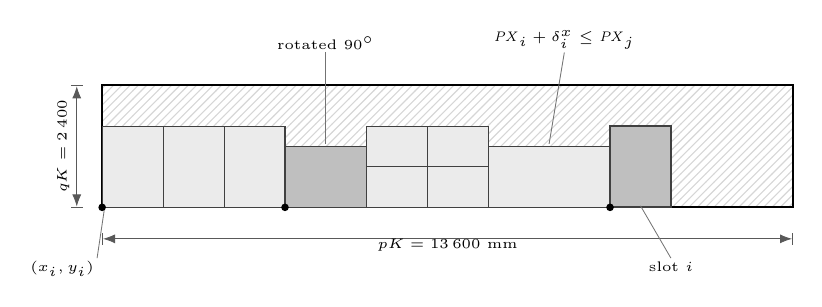
\begin{tikzpicture}[x=0.645cm, y=0.645cm, >=Latex,
  fp/.style={draw=black!75, fill=black!8, line width=0.4pt},
  hl/.style={draw=black!75, fill=black!25, line width=0.4pt},
  tny/.style={font=\tiny, align=center, inner sep=1pt},
  led/.style={black!55, line width=0.3pt}]
  % trailer floor, 13.6 x 2.4 (decimetres of the real 13 600 x 2 400 mm)
  \fill[pattern=north east lines, pattern color=black!16]
     (0,0) rectangle (13.6,2.4);
  \draw[line width=0.7pt] (0,0) rectangle (13.6,2.4);

  % 1200 x 1600 footprints
  \foreach \x in {0,1.2,2.4} \draw[fp] (\x,0) rectangle ++(1.2,1.6);
  % one rotated 90 degrees: 1600 x 1200
  \draw[hl] (3.6,0) rectangle ++(1.6,1.2);
  % 1200 x 800 footprints
  \foreach \x/\y in {5.2/0, 5.2/0.8, 6.4/0, 6.4/0.8}
     \draw[fp] (\x,\y) rectangle ++(1.2,0.8);
  % 2400 x 1200
  \draw[fp] (7.6,0) rectangle ++(2.4,1.2);
  % the lifted slot i
  \draw[hl, line width=0.8pt] (10.0,0) rectangle ++(1.2,1.6);

  % bottom-left corners
  \foreach \x/\y in {0/0, 3.6/0, 10.0/0} \fill[black] (\x,\y) circle (0.075);

  % dimensions
  \draw[|<->|, black!65, line width=0.3pt] (0,-0.62) -- (13.6,-0.62);
  \node[tny, anchor=north] at (6.8,-0.56) {$pK=13\,600$ mm};
  \draw[|<->|, black!65, line width=0.3pt] (-0.50,0) -- (-0.50,2.4);
  \node[tny, rotate=90, anchor=south] at (-0.58,1.2) {$qK=2\,400$};

  % annotations outside the floor, with leaders
  \node[tny, anchor=south] (rot) at (4.4,3.05) {rotated $90^{\circ}$};
  \draw[led] (rot.south) -- (4.4,1.25);
  \node[tny, anchor=south] (nov) at (9.1,3.05)
     {$\mathit{PX}_{i}+\delta^{x}_{i}\le \mathit{PX}_{j}$};
  \draw[led] (nov.south) -- (8.8,1.25);
  \node[tny, anchor=north west] (sl) at (10.7,-1.00) {slot $i$};
  \draw[led] (sl.north) -- (10.6,0.03);
  \node[tny, anchor=north east] (bl) at (-0.10,-1.00) {$(x_{i},y_{i})$};
  \draw[led] (bl.north east) -- (0.04,-0.06);
\end{tikzpicture}
\caption{the floor, \eqref{bp:PP-nonov-x1}--\eqref{bp:PP-cont-x}}
\label{fig:truck-floor}
\end{subfigure}\hfill
\begin{subfigure}[b]{0.30\textwidth}
\centering
\tdplotsetmaincoords{72}{128}
\begin{tikzpicture}[tdplot_main_coords, scale=0.70, >=Latex,
  tny/.style={font=\tiny, align=left, inner sep=1pt}]
  % four homogeneous layers in one slot, two shades: the per-slot assignment
  \drawblock{0}{0}{0}{1.2}{1.6}{0.62}{stkA}{0}{0}{1}
  \drawblock{0}{0}{1.24}{1.2}{1.6}{0.62}{stkB}{0}{0}{1}
  % height budget
  \draw[|<->|, black!70, line width=0.3pt] (1.55,0,0) -- (1.55,0,2.48);
  \node[tny, anchor=west] at (2.90,0,1.55)
     {$\sum_{r} r_{pr}\ell_{ir}$\\ $\le rK$};
  % crush cap at the base
  \node[tny, anchor=north] at (0.6,0.8,-0.30)
     {$\sum_{n}w_{n}v_{in}\le W^{\max}$};
  \node[tny, anchor=south] at (0.6,0.8,2.95)
     {$v_{in}$: two products,\\ one per layer};
\end{tikzpicture}
\caption{one slot, \eqref{eq:col-height} and \eqref{eq:col-crush}}
\label{fig:truck-stack}
\end{subfigure}
\caption{What the pricing problem designs. A column is a drawing a
loading crew could execute: footprints placed on the floor without
overlap and inside $pK\times qK$, each slot a stack of homogeneous
layers under the height budget \eqref{bp:PP-height} and the per-slot
crush cap, the load assigned to the slots in the same period so that
$b_{\omega n}=\sum_{i\le m}v_{in}$, and the whole truck full on the
binding resource \eqref{bp:PP-util}--\eqref{bp:PP-utilw}: volume
\emph{or} payload, $\max\{\gamma/\Gamma_{K},\,w/pK^{w}\}\ge\alpha$, and
never the sum of the two ratios.}
\label{fig:truck}
\end{figure}


\paragraph{What pricing cannot return.}
For any dual vector \eqref{bp:PP-objective} is linear in the image, so
it attains its optimum at an extreme point of
$\operatorname{conv}(\Omega^{g})$: pricing returns extreme loads only.
A balanced load inside the hull is dominated componentwise by a
fractional blend of single-commodity trucks --- the relaxation buys
that blend for one truck where an integer plan pays for each truck it
mixes --- so no choice of duals returns it, however the search moves
them (Figure~\ref{fig:hull}). Interior loads are precisely what an
integer plan needs when a period's demand does not decompose into full
trucks, which is why the method does not ask pricing for them. The
flow-first construction of Section~\ref{sec:relaxfix-flow} reaches the
interior directly, and branching on the fleet aggregates withdraws the
dominating column, so the duals move and the oracle is asked for a load
the pool does not yet hold.

\begin{figure}[!ht]
\centering
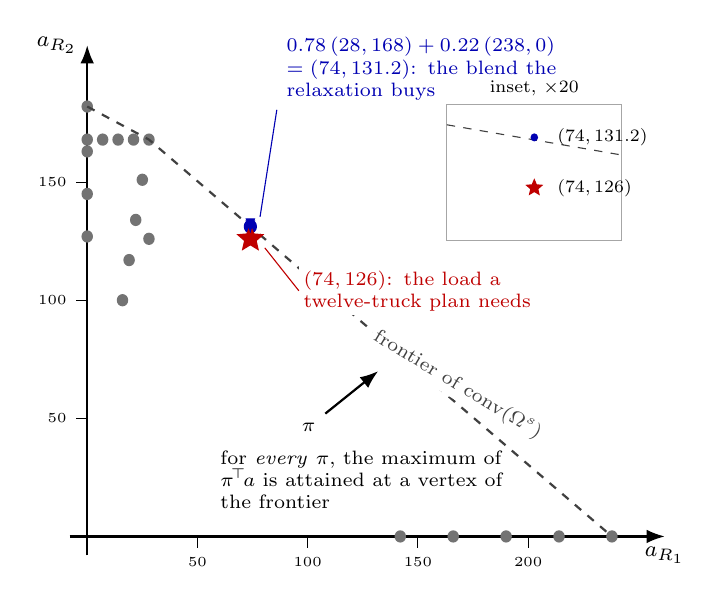
\begin{tikzpicture}[x=0.028cm, y=0.030cm, >=Latex,
  lab/.style={font=\scriptsize, align=left},
  lead/.style={black!55, thin, shorten >=2pt}]
  % axes
  \draw[->, thick] (-8,0) -- (262,0) node[below] {\footnotesize $a_{R_1}$};
  \draw[->, thick] (0,-8) -- (0,208) node[left] {\footnotesize $a_{R_2}$};
  \foreach \x in {50,100,150,200} \draw (\x,0) -- (\x,-5) node[below] {\tiny \x};
  \foreach \y in {50,100,150} \draw (0,\y) -- (-5,\y) node[left] {\tiny \y};

  % loads produced by the demand-derived price sweep (the seed pool)
  \foreach \p in {(0,127),(0,145),(0,163),(0,168),(0,182),(7,168),(14,168),
                  (16,100),(19,117),(21,168),(22,134),(25,151),(28,126),
                  (28,168),(142,0),(166,0),(190,0),(214,0),(238,0)}
      \fill[black!55] \p circle[radius=2.6];

  % upper-right frontier of the convex hull
  \draw[black!75, dashed, thick] (0,182) -- (28,168) -- (238,0);
  \node[lab, black!75, fill=white, inner sep=1.5pt, rotate=-31] at (168,64) {frontier of $\operatorname{conv}(\Omega^{s})$};

  % dominating blend, and the load an integer plan needs
  \fill[blue!70!black] (74,131.2) circle[radius=3];
  \node[star, star points=5, star point ratio=2.2, fill=red!75!black,
        inner sep=1.7pt] at (74,126) {};
  \draw[blue!70!black, <->, thin] (74,129) -- (74,128.2);

  \node[lab, blue!70!black, anchor=west, text width=40mm] (bl) at (86,198)
      {$0.78\,(28,168)+0.22\,(238,0)$\\ $=(74,131.2)$: the blend the\\
       relaxation buys};
  \draw[lead, blue!70!black] (bl.south west) -- (78,133);

  \node[lab, red!75!black, fill=white, inner sep=1.5pt, anchor=west, text width=38mm] (tg) at (96,104)
      {$(74,126)$: the load a\\ twelve-truck plan needs};
  \draw[lead, red!75!black] (tg.west) -- (79,124);

  % a dual vector, drawn inside the hull where there is room
  \draw[->, thick] (108,52) -- ++(24,18);
  \node[lab, anchor=north east] at (108,52) {$\pi$};
  \node[lab, anchor=west, text width=36mm] at (56,24)
      {for \emph{every} $\pi$, the maximum of $\pi^{\!\top}\!a$ is attained
       at a vertex of the frontier};
  % inset: the blend and the load an integer plan needs are 5.2 units apart on a
  % 208-unit axis, so they read as one mark at print size.
  \begin{scope}[shift={(176,138)}, x=0.30cm, y=0.32cm]
     \draw[black!35] (-1.2,-1.2) rectangle (6.2,4.2);
     \draw[black!75, dashed] (-1.2,3.4) -- (6.2,2.2);
     \fill[blue!70!black] (2.5,2.9) circle[radius=0.16];
     \node[star, star points=5, star point ratio=2.2, fill=red!75!black,
           inner sep=1.1pt] at (2.5,0.9) {};
     \node[lab, anchor=west, scale=0.9] at (3.1,2.9) {$(74,131.2)$};
     \node[lab, anchor=west, scale=0.9] at (3.1,0.9) {$(74,126)$};
     \node[lab, anchor=south, scale=0.9] at (2.5,4.2) {inset, $\times 20$};
  \end{scope}
\end{tikzpicture}
\caption{Why the load a cheaper plan needs is never priced. Dots are
the supplier-bound loads obtained from a sweep of demand-derived price
vectors; the dashed line is the upper-right frontier of their convex
hull. The pricing objective is linear, so for \emph{any} dual vector
$\pi$ its optimum is attained at a vertex of that frontier. The load
$(74,126)$ lies strictly below it --- it is dominated componentwise by
the blend $0.78\,(28,168)+0.22\,(238,0)=(74,131.2)$ --- so no choice of
duals returns it. The relaxation buys that blend for one truck, while
an integer plan must pay for both of the trucks it mixes. The construction of
Section~\ref{sec:relaxfix-flow} reaches the interior directly: it
partitions a delivery vector into legal loads instead of asking a
linear objective for them.}
\label{fig:hull}
\end{figure}


\section{Branching, with the flow-first construction inside it}
\label{sec:branching}

The branching hierarchy is read off the robustness criterion of
Section~\ref{sec:rmp}. A row with $\phi\equiv1$ --- any bound on a sum of
dispatch counts, including the per-class total $n_{gt}$ and the fleet
$X=\sum_{g,t}n_{gt}$ --- has its dual folded into $\mu_{gt}$ exactly as
\eqref{bp:MP-count} does, and all such aggregates are integer in every
plan. A row with $\phi$ affine in the image, a bound on
$\overline{V}_{nt}$ or $\overline{V^{\mathrm{e}}}_{rt}$, is absorbed
into $\pi_{ct}$, already an input of the pricing problem; these count
physical RTIs, so they too may carry a dichotomy. Bounding a single
$\lambda^{g}_{\omega t}$ is neither: honouring it means excluding that
column from the subproblem
\autocite{Vanderbeck2000OnIntegerProgramming}, destroying the property
that one column set serves every period. It is also useless here, the
master holding many columns that differ in a single RTI, so the
relaxation answers by shifting the same fractional weight one column
over --- measured at $3\,000$ branches with no integral relaxation
reached.

Between the two robust rungs the first binds, because transport cost
is $cK\cdot X$ and nothing else in the objective counts trucks. A bound
on a delivery is answered by moving freight between periods at the
price of one period's holding cost, and so is a bound on a
\emph{single} period's dispatch total; the aggregate with no such
escape is the horizon total. We therefore branch on the fleet, in two
levels (Figure~\ref{fig:tree}), keeping the delivery rung as a third
entered only where the first two have nothing left to say. Master,
pricing problem, construction and tree are together the procedure we
call BP-3D-SCPTOP (Algorithm~\ref{alg:bp3d}).

\paragraph{Level 1: the total fleet.}
Given an incumbent with fleet vector $\mathbf{n}^{\star}$ and total
$X^{\star}$, three regions partition the space. $X\ge X^{\star}+1$
costs a whole truck with no offset and is usually pruned by bound;
$X=X^{\star}$ fixes transport, so everything inside it is inventory
allocation and this is where level 2 goes; and $X\le X^{\star}-1$ is
the only region that can beat the incumbent outright, so it is worth a
certificate of its own and the stack is ordered to expand it first. A
plan found \emph{inside} an inequality region splits it on its own
total the same way, so level 1 recurses.

\paragraph{Level 2: the fleet vector, inside $X=X^{\star}$.}
Fix an order on the pairs $(g,t)$. The fleet vector of any plan in the
region differs from $\mathbf{n}^{\star}$ at a first index $j$, or
nowhere, so branching there gives three children,
\begin{equation}
n_{j}\le n^{\star}_{j}-1,
\qquad
n_{j}= n^{\star}_{j},
\qquad
n_{j}\ge n^{\star}_{j}+1,
\label{eq:murty}
\end{equation}
disjoint and exhaustive, with the equality child partitioned again at
$j+1$ (Murty's scheme \autocite{Murty1968AnAlgorithm}) and expanded
first. The partition is taken around the plan \emph{constructed at that
node}, so a node that improves the incumbent is re-partitioned around
the better plan at once and nothing is restarted.

% F6 of article/paper-figures.md, redrawn, and the only drawing of the
% branching scheme.  One picture for the whole hierarchy: the three rungs,
% nested (level 2 inside the equality child of level 1, level 3 inside the
% Murty leaf); an integer line under the first split, so that "disjoint and
% exhaustive" is shown rather than asserted and the later rungs can be read
% off it; the construction as what happens at every node; and the rung that
% is deliberately not taken.  Greyscale only, straight edges only, every
% label clear of every edge, and the spine of the tree runs at x=7.5 -- the
% heading blocks are 66mm wide so that none of them reaches it.
\begin{figure}[!t]
\centering
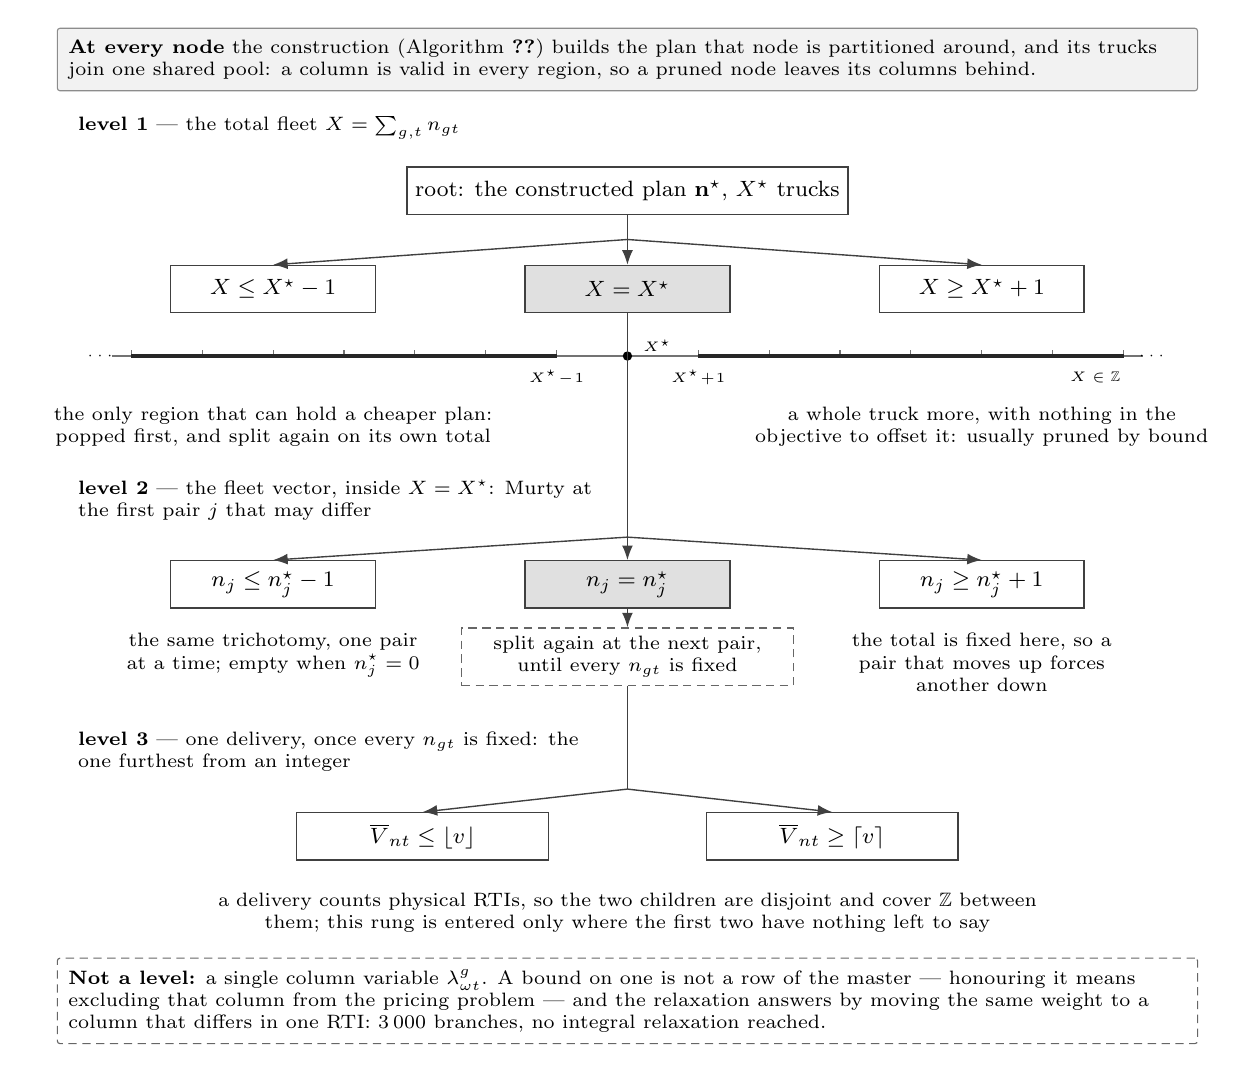
\begin{tikzpicture}[>=Latex, x=1cm, y=1cm,
  nd/.style={rectangle, draw=black!75, fill=white, line width=0.5pt,
             inner sep=3pt, minimum width=26mm, minimum height=6mm,
             font=\footnotesize},
  fx/.style={nd, fill=black!12},
  rt/.style={nd, minimum width=52mm},
  rep/.style={rectangle, draw=black!60, densely dashed, fill=white,
              line width=0.5pt, inner sep=3pt, text width=40mm,
              align=flush center, font=\scriptsize},
  an/.style={font=\scriptsize, align=flush center, text width=60mm, anchor=north},
  hd/.style={font=\scriptsize, align=flush left, anchor=north west,
             text width=66mm},
  bnr/.style={rectangle, draw=black!45, fill=black!5, rounded corners=1pt,
              inner sep=4pt, text width=142mm, align=flush left, font=\scriptsize,
              anchor=north},
  bnx/.style={bnr, draw=black!60, densely dashed, fill=white},
  sp/.style={draw=black!75, line width=0.5pt},
  ed/.style={sp, ->},
  ax/.style={draw=black!55, line width=0.4pt},
  seg/.style={draw=black!85, line width=1.5pt},
  tk/.style={font=\tiny, inner sep=1pt}]

% ---------------------------------------------------------------- banner --
\node[bnr] (ban) at (7.5,1.62) {\textbf{At every node} the construction
  (Algorithm~\ref{alg:construct}) builds the plan that node is partitioned
  around, and its trucks join one shared pool: a column is valid in every
  region, so a pruned node leaves its columns behind.};

% =============================================================== level 1 ==
\node[hd] at (0.4,0.62) {\textbf{level 1} --- the total fleet
  $X=\sum_{g,t}n_{gt}$};

\node[rt] (root) at (7.5,-0.45)
  {root: the constructed plan $\mathbf{n}^{\star}$, $X^{\star}$ trucks};

\node[nd] (a1) at (3.0,-1.70) {$X\le X^{\star}-1$};
\node[fx] (b1) at (7.5,-1.70) {$X=X^{\star}$};
\node[nd] (c1) at (12.0,-1.70) {$X\ge X^{\star}+1$};
\coordinate (j1) at (7.5,-1.07);
\draw[sp] (root.south) -- (j1);
\draw[ed] (j1) -- (a1.north);
\draw[ed] (j1) -- (b1.north);
\draw[ed] (j1) -- (c1.north);

% the integer line: the three children abut at $X^\star$ and leave no gap
\draw[ax] (0.95,-2.55) -- (14.05,-2.55);
\foreach \i in {0,...,14} {\draw[ax] (1.2+\i*0.9,-2.55) -- ++(0,0.075);}
\draw[seg] (1.2,-2.55) -- (6.6,-2.55);
\draw[seg] (8.4,-2.55) -- (13.8,-2.55);
\fill (7.5,-2.55) circle (1.7pt);
\node[tk, anchor=east] at (1.05,-2.55) {$\cdots$};
\node[tk, anchor=west] at (13.95,-2.55) {$\cdots$};
\node[tk] at (6.6,-2.82) {$X^{\star}\!-\!1$};
\node[tk] at (8.4,-2.82) {$X^{\star}\!+\!1$};
\node[tk, anchor=west] at (7.66,-2.42) {$X^{\star}$};
\node[tk, anchor=east] at (13.8,-2.82) {$X\in\mathbb{Z}$};

\node[an] at (3.0,-3.07) {the only region that can hold a cheaper plan:
  popped first, and split again on its own total};
\node[an] at (12.0,-3.07) {a whole truck more, with nothing in the objective
  to offset it: usually pruned by bound};

% =============================================================== level 2 ==
\node[hd] at (0.4,-4.00) {\textbf{level 2} --- the fleet vector, inside
  $X=X^{\star}$: Murty at the first pair $j$ that may differ};

\node[nd] (a2) at (3.0,-5.45) {$n_{j}\le n^{\star}_{j}-1$};
\node[fx] (b2) at (7.5,-5.45) {$n_{j}=n^{\star}_{j}$};
\node[nd] (c2) at (12.0,-5.45) {$n_{j}\ge n^{\star}_{j}+1$};
\coordinate (j2) at (7.5,-4.85);
\draw[sp] (b1.south) -- (7.5,-2.55);
\draw[sp] (7.5,-2.55) -- (j2);
\draw[ed] (j2) -- (a2.north);
\draw[ed] (j2) -- (b2.north);
\draw[ed] (j2) -- (c2.north);

\node[an, text width=38mm] at (3.0,-5.95) {the same trichotomy, one pair at
  a time; empty when $n^{\star}_{j}=0$};
\node[an, text width=38mm] at (12.0,-5.95) {the total is fixed here, so a pair
  that moves up forces another down};

\node[rep] (rep) at (7.5,-6.37) {split again at the next pair,\\
  until every $n_{gt}$ is fixed};
\draw[ed] (b2.south) -- (rep.north);

% =============================================================== level 3 ==
\node[hd] at (0.4,-7.20) {\textbf{level 3} --- one delivery, once every
  $n_{gt}$ is fixed: the one furthest from an integer};

\node[nd, minimum width=32mm] (a3) at (4.9,-8.65)
  {$\overline{V}_{nt}\le\lfloor v\rfloor$};
\node[nd, minimum width=32mm] (c3) at (10.1,-8.65)
  {$\overline{V}_{nt}\ge\lceil v\rceil$};
\coordinate (j3) at (7.5,-8.05);
\draw[sp] (rep.south) -- (j3);
\draw[ed] (j3) -- (a3.north);
\draw[ed] (j3) -- (c3.north);

\node[an, text width=104mm] at (7.5,-9.25) {a delivery counts physical RTIs,
  so the two children are disjoint and cover $\mathbb{Z}$ between them; this
  rung is entered only where the first two have nothing left to say};

% --------------------------------------------------------- the non-rung --
\node[bnx] (ban2) at (7.5,-10.19) {\textbf{Not a level:} a single column
  variable $\lambda^{g}_{\omega t}$. A bound on one is not a row of the
  master --- honouring it means excluding that column from the pricing
  problem --- and the relaxation answers by moving the same weight to a
  column that differs in one RTI: $3\,000$ branches, no integral relaxation
  reached.};

\end{tikzpicture}
\caption{Every rung bounds an integer quantity the master already prices,
so the children of a split are disjoint and together exhaustive and the search
gives up nothing by taking them. The order is forced by the objective:
transport costs $cK\cdot X$ and nothing else in the model counts trucks, so
the horizon total is the one aggregate that cannot be answered by moving
freight between periods for one period's holding cost, as a single dispatch
count or a single delivery can. And because these are rows of the master and
not restrictions on the subproblem, branching moves the duals and leaves the
pricing problem alone --- which is also how a load no dual vector would have
asked for (Figure~\ref{fig:hull}) comes to be priced at all.}
\label{fig:tree}
\end{figure}


\paragraph{Pruning, and what counts as a proof.}
A node is a region imposed on the RMP as fleet rows. Its LP over the
current pool is solved first as a filter (Section~\ref{sec:bounds});
where the filter allows pruning and the certification policy admits the
node, column generation is run to a certificate, and a certified value
at or above the incumbent prunes it while a value below becomes that
region's bound. Every other node carries its parent's, valid because
the child's region is a subset. An infeasible node relaxation is
\emph{not} a proof that a region is empty: stock non-negativity is not
elastic, so a fleet lower bound can force deliveries up through
whatever columns the pool holds and kill the relaxation for a reason
internal to the pool. Only arithmetic licenses that sentence, and three
such arguments are available: the fleet box intersected with the
interval on $X$, an availability cap telescoped from the sending rows
\eqref{sb:eq:inve-plant} and \eqref{sb:eq:inv-sup-main} under
non-negative stock, and the constants of \eqref{eq:covercut} read as a
requirement floor.

\paragraph{What the tree reports.}
The incumbent is the cheapest verified plan any construction found. The
global bound is the minimum over the \emph{frontier}, not the root, a
region nobody expanded contributing nothing; at the deadline the open
regions are swept and certified where the filter allows. Under 3D
loading a region's certificate comes, like the root's, from the
volumetric relaxation with the region's fleet rows applied, which
Proposition~\ref{prop:inclusion} covers because those rows bound the
fleet vector and not the load model. A column, by contrast, is a
feasible load, so one found in any region is valid in every other and a
pruned node leaves its columns behind. Optimality is claimed
\emph{only} when the root is certified, no region remains open, no
restart has broken the partition and the incumbent meets the global
bound. The hierarchy is finite and its levels exhaustive, so those
conditions are reachable in principle; no run here meets them.

\begin{algorithm}[!htb]
\caption{BP-3D-SCPTOP: branch and bound over the fleet vector, with
\textsc{Construct} as primal heuristic and \textsc{Certify} as bound.}
\label{alg:bp3d}
\begin{algorithmic}[1]
\State $\bar\Omega\gets$ one maximally full single-commodity truck per commodity
   and direction, each verified
   \Comment{no demand mixes, no reduced variants}
\State $\mathrm{LB}_{0}\gets\textsc{Certify}(\bar\Omega,\text{root})$;
   $(\bar z,\mathbf{n}^{\star},\bar\Omega)\gets\textsc{Construct}(\bar\Omega,\text{root})$;
   $X^{\star}\gets\sum_{g,t}n^{\star}_{gt}$
\State $\mathcal{S}\gets[\,X\ge X^{\star}+1,\; X=X^{\star},\; X\le X^{\star}-1\,]$
   \Comment{a stack: the region that can beat the incumbent is popped first}
\While{$\mathcal{S}\ne\emptyset$ and time remains}
   \State $\mathcal{R}\gets$ pop $\mathcal{S}$; impose it on the RMP as fleet rows
   \If{$\mathcal{R}$ is refuted arithmetically} \State \textbf{continue}
      \Comment{fleet box, availability, requirement} \EndIf
   \State $\tilde z\gets$ LP over $\bar\Omega$ inside $\mathcal{R}$
      \Comment{over-estimates the region's LP: a filter, never a bound}
   \If{$\tilde z\ge\bar z$ and the policy certifies $\mathcal{R}$}
      \State $(\mathrm{LB}_{\mathcal{R}},\text{proved})\gets
             \textsc{Certify}(\bar\Omega,\mathcal{R})$
      \If{$\mathrm{LB}_{\mathcal{R}}\ge\bar z$} \State \textbf{continue}
         \Comment{pruned} \EndIf
      \State record $\mathrm{LB}_{\mathcal{R}}$ as an open bound
   \Else \State $\mathcal{R}$ carries its parent's bound \EndIf
   \State $(z,\hat{\mathbf{n}},\bar\Omega)\gets\textsc{Construct}(\bar\Omega,\mathcal{R})$
      \Comment{its columns join the shared pool whatever it returns}
   \If{no plan} \State price under $\mathcal{R}$'s duals and construct once
      more; \textbf{continue} if still none \EndIf
   \If{$z<\bar z$} \State $(\bar z,\mathbf{n}^{\star})\gets(z,\hat{\mathbf{n}})$
      \Comment{new incumbent} \EndIf
   \If{$\mathcal{R}$ does not fix $X$}
      \State push the three regions of level 1 around
            $\sum_{g,t}\hat n_{gt}$ \Comment{level 1 recurses}
   \ElsIf{the Murty depth $j$ is below the cap}
      \State push the three children \eqref{eq:murty} at the $j$-th pair,
             around $\hat{\mathbf{n}}$, equality last
   \EndIf
\EndWhile
\ForAll{$\mathcal{R}$ still on $\mathcal{S}$, while a reserve of time remains}
   \State filter by the pool LP; certify the survivors; record their bounds
   \Comment{the frontier}
\EndFor
\State $\mathrm{LB}\gets\max\{\mathrm{LB}_{0},\,
   \min\text{ over the open and frontier bounds}\}$, capped at $\bar z$
\State verify every dispatched truck of the incumbent against
   \eqref{eq:col-geom}--\eqref{eq:col-agg}
\State \Return $(\bar z,\mathrm{LB})$; optimality is claimed only if
   $\mathrm{LB}_{0}$ was proved, $\mathcal{S}=\emptyset$, no restart occurred
   and $\bar z=\mathrm{LB}$
\end{algorithmic}
\end{algorithm}


\subsection{The initial pool}
\label{sec:initcols}
The search starts from the plainest possible pool: one maximally full
truck per commodity and direction, obtained geometrically by pricing
that commodity alone with every other capped at zero --- so that where
the probe closes, the pool truck is that commodity's placeable maximum
and the same number is its placeability cap --- and volumetrically by
filling to capacity. No demand mixes and no reduced variants are
seeded, so whatever the search reaches it reached by pricing, branching
and construction.

\subsection{The flow-first construction}
\label{sec:relaxfix-flow}

The primal heuristic decides first how much moves and how many trucks
carry it, and builds the trucks afterwards. It runs inside the region
$\mathcal{R}$ of the node that calls it and must stay there, or the
children that node induces would partition around a point it excludes,
and it runs on a \emph{fresh copy} of the restricted master, step~2
changing variable types the node's own LP needs intact.
Figure~\ref{fig:construct} follows one period through the four steps of
Algorithm~\ref{alg:construct}.

% F5 of article/paper-figures.md: the flow-first construction, one period,
% top to bottom.  The object passing between the steps is drawn, not named,
% and every band carries the same two-line statement of what it fixes and
% what it leaves free.  Greyscale only (fills black!X plus one hatch), so
% nothing depends on colour.  The libraries used -- patterns,
% decorations.pathreplacing, arrows.meta -- are all loaded by
% ../necessarypackages and paper.tex; no new package is needed.
\begin{figure}[!htb]
\centering
\resizebox{\textwidth}{!}{%
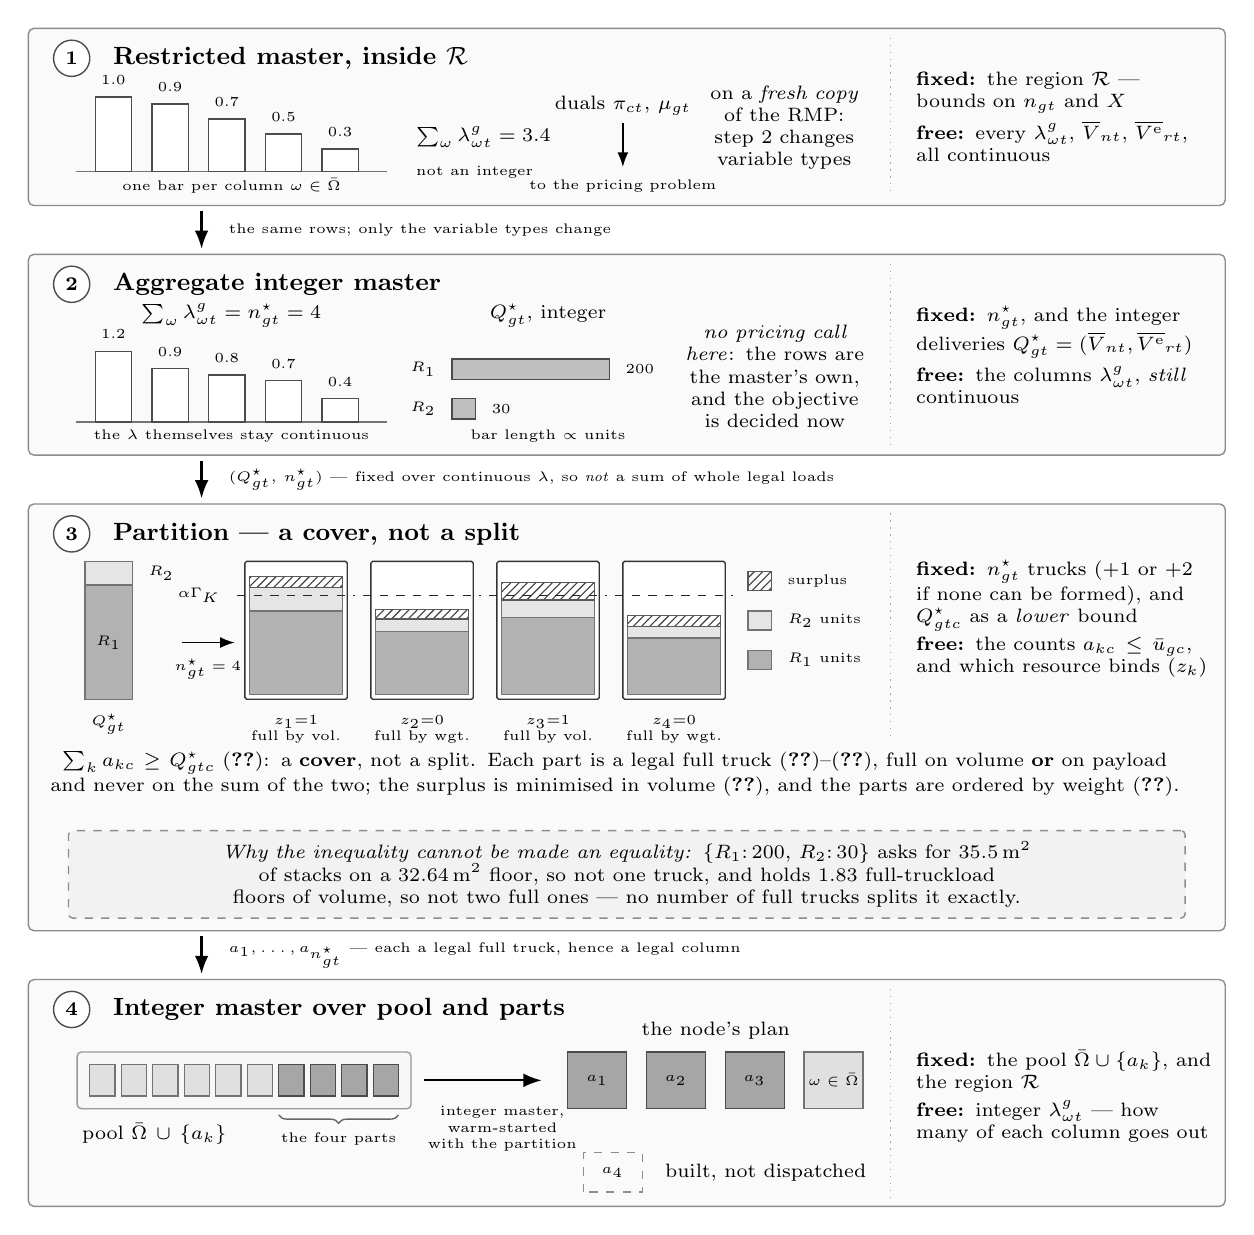
\begin{tikzpicture}[>=Latex, line width=0.5pt,
  band/.style={draw=black!45, fill=black!2, rounded corners=2pt},
  ttl/.style={font=\small\bfseries, anchor=west, align=left},
  bdg/.style={circle, draw=black!70, fill=white, inner sep=0pt,
              minimum size=4.6mm, font=\scriptsize\bfseries},
  ann/.style={font=\scriptsize, align=center},
  annl/.style={font=\scriptsize, align=left},
  mic/.style={font=\tiny, align=center},
  micl/.style={font=\tiny, align=left},
  st/.style={font=\scriptsize, align=left, anchor=west, text width=38mm},
  barO/.style={draw=black!70, fill=white},         % still continuous
  qty/.style={draw=black!70, fill=black!25},
  trk/.style={draw=black!80, fill=white, rounded corners=0.6pt},
  seg1/.style={draw=black!55, fill=black!30},      % R1 units
  seg2/.style={draw=black!55, fill=black!10},      % R2 units
  sur/.style={draw=black!65, pattern=north east lines, pattern color=black!75},
  glyA/.style={draw=black!55, fill=black!12},      % a column already in the pool
  glyB/.style={draw=black!70, fill=black!35},      % a part built here
  rule/.style={draw=black!35, dotted}]

\def\BW{15.2}          % content width
\def\SX{10.95}         % the fixed/free rule
\def\GX{2.20}          % x of the between-band arrows

% =====================================================================
% band 1 -- the node's LP
% =====================================================================
\draw[band] (0,0) rectangle (\BW,-2.25);
\draw[rule] (\SX,-0.12) -- (\SX,-2.13);
\node[bdg] at (0.55,-0.38) {1};
\node[ttl] at (0.95,-0.38) {Restricted master, inside $\mathcal{R}$};

\draw[black!55] (0.60,-1.82) -- (4.55,-1.82);
\foreach \i/\h/\v in {0/0.95/{1.0}, 1/0.86/{0.9}, 2/0.67/{0.7},
                      3/0.48/{0.5}, 4/0.29/{0.3}} {
  \pgfmathsetmacro{\x}{0.85+\i*0.72}
  \draw[barO] (\x,-1.82) rectangle (\x+0.46,-1.82+\h);
  \node[mic, anchor=south] at (\x+0.23,-1.79+\h) {\v};
}
\node[mic] at (2.58,-2.00) {one bar per column $\omega\in\bar\Omega$};
\node[annl, anchor=west] at (4.80,-1.38)
  {$\sum_{\omega}\lambda^{g}_{\omega t}=3.4$};
\node[mic, anchor=north west] at (4.80,-1.62) {not an integer};

\node[ann] at (7.55,-0.98) {duals $\pi_{ct},\,\mu_{gt}$};
\draw[->] (7.55,-1.20) -- (7.55,-1.76);
\node[mic, anchor=north] at (7.55,-1.80) {to the pricing problem};

\node[ann, text width=22mm] at (9.60,-1.26)
  {on a \emph{fresh copy} of the RMP: step~2 changes variable types};

\node[st] at (11.15,-1.12)
  {\textbf{fixed:} the region $\mathcal{R}$ --- bounds on $n_{gt}$ and $X$\\[2pt]
   \textbf{free:} every $\lambda^{g}_{\omega t}$, $\overline{V}_{nt}$,
   $\overline{V^{\mathrm{e}}}_{rt}$, all continuous};

% ---- 1 -> 2 ----------------------------------------------------------
\draw[->, line width=0.8pt] (\GX,-2.32) -- (\GX,-2.80);
\node[micl, anchor=west] at (\GX+0.22,-2.56)
  {the same rows; only the variable types change};

% =====================================================================
% band 2 -- the aggregate integer master
% =====================================================================
\draw[band] (0,-2.87) rectangle (\BW,-5.42);
\draw[rule] (\SX,-2.99) -- (\SX,-5.30);
\node[bdg] at (0.55,-3.25) {2};
\node[ttl] at (0.95,-3.25) {Aggregate integer master};

\draw[black!55] (0.60,-5.00) -- (4.55,-5.00);
\foreach \i/\h/\v in {0/0.90/{1.2}, 1/0.68/{0.9}, 2/0.60/{0.8},
                      3/0.53/{0.7}, 4/0.30/{0.4}} {
  \pgfmathsetmacro{\x}{0.85+\i*0.72}
  \draw[barO] (\x,-5.00) rectangle (\x+0.46,-5.00+\h);
  \node[mic, anchor=south] at (\x+0.23,-4.97+\h) {\v};
}
\node[ann, anchor=south] at (2.58,-3.92)
  {$\sum_{\omega}\lambda^{g}_{\omega t}=n^{\star}_{gt}=4$};
\node[mic] at (2.58,-5.18) {the $\lambda$ themselves stay continuous};

\node[ann, anchor=south] at (6.60,-3.92) {$Q^{\star}_{gt}$, integer};
\node[mic, anchor=east] at (5.30,-4.33) {$R_{1}$};
\draw[qty] (5.38,-4.46) rectangle (7.38,-4.20);
\node[mic, anchor=west] at (7.46,-4.33) {200};
\node[mic, anchor=east] at (5.30,-4.83) {$R_{2}$};
\draw[qty] (5.38,-4.96) rectangle (5.68,-4.70);
\node[mic, anchor=west] at (5.76,-4.83) {30};
\node[mic] at (6.60,-5.18) {bar length $\propto$ units};

\node[ann, text width=25mm] at (9.48,-4.42)
  {\emph{no pricing call here}: the rows are the master's own, and the
   objective is decided now};

\node[st] at (11.15,-4.15)
  {\textbf{fixed:} $n^{\star}_{gt}$, and the integer deliveries
   $Q^{\star}_{gt}=(\overline{V}_{nt},\overline{V^{\mathrm{e}}}_{rt})$\\[2pt]
   \textbf{free:} the columns $\lambda^{g}_{\omega t}$, \emph{still} continuous};

% ---- 2 -> 3 ----------------------------------------------------------
\draw[->, line width=0.8pt] (\GX,-5.49) -- (\GX,-5.97);
\node[micl, anchor=west] at (\GX+0.22,-5.73)
  {$(Q^{\star}_{gt},\,n^{\star}_{gt})$ --- fixed over continuous $\lambda$,
   so \emph{not} a sum of whole legal loads};

% =====================================================================
% band 3 -- the partition, as a cover
% =====================================================================
\draw[band] (0,-6.04) rectangle (\BW,-11.46);
\draw[rule] (\SX,-6.16) -- (\SX,-8.98);
\node[bdg] at (0.55,-6.42) {3};
\node[ttl] at (0.95,-6.42) {Partition --- a cover, not a split};

% what has to be delivered
\draw[seg1] (0.72,-8.52) rectangle (1.32,-7.07);
\draw[seg2] (0.72,-7.07) rectangle (1.32,-6.77);
\node[mic] at (1.02,-7.80) {$R_{1}$};
\node[mic, anchor=west] at (1.40,-6.92) {$R_{2}$};
\node[mic, anchor=north] at (1.02,-8.58) {$Q^{\star}_{gt}$};
\draw[->] (1.95,-7.80) -- (2.62,-7.80);
\node[mic, anchor=east] at (2.56,-7.20) {$\alpha\Gamma_{K}$};
\node[mic, anchor=north] at (2.28,-7.88) {$n^{\star}_{gt}=4$};

% the four parts
\foreach \k/\f/\r/\s/\z/\b in {%
   1/1.56/1.12/0.14/{$z_{1}{=}1$}/{full by vol.},
   2/1.14/0.86/0.12/{$z_{2}{=}0$}/{full by wgt.},
   3/1.48/1.04/0.22/{$z_{3}{=}1$}/{full by vol.},
   4/1.06/0.78/0.14/{$z_{4}{=}0$}/{full by wgt.}} {
  \pgfmathsetmacro{\x}{2.75+(\k-1)*1.60}
  \pgfmathsetmacro{\yr}{-8.52+\r}
  \pgfmathsetmacro{\yf}{-8.52+\f}
  \pgfmathsetmacro{\ys}{\yf-\s}
  \draw[trk] (\x,-8.52) rectangle (\x+1.30,-6.77);
  \draw[seg1] (\x+0.06,-8.46) rectangle (\x+1.24,\yr);
  \draw[seg2] (\x+0.06,\yr) rectangle (\x+1.24,\ys);
  \draw[sur]  (\x+0.06,\ys) rectangle (\x+1.24,\yf);
  \draw[dashed, black!85] (\x-0.10,-7.20) -- (\x+1.40,-7.20);
  \node[mic, text width=15mm, anchor=north] at (\x+0.65,-8.60) {\z\\ \b};
}

% key
\draw[sur]  (9.14,-7.14) rectangle (9.44,-6.90);
\node[mic, anchor=west] at (9.52,-7.02) {surplus};
\draw[seg2] (9.14,-7.64) rectangle (9.44,-7.40);
\node[mic, anchor=west] at (9.52,-7.52) {$R_{2}$ units};
\draw[seg1] (9.14,-8.14) rectangle (9.44,-7.90);
\node[mic, anchor=west] at (9.52,-8.02) {$R_{1}$ units};

\node[st] at (11.15,-7.50)
  {\textbf{fixed:} $n^{\star}_{gt}$ trucks ($+1$ or $+2$ if none can be
   formed), and $Q^{\star}_{gtc}$ as a \emph{lower} bound\\[2pt]
   \textbf{free:} the counts $a_{kc}\le\bar u_{gc}$, and which resource
   binds ($z_{k}$)};

\node[ann, text width=144mm, anchor=north] at (7.45,-9.06)
  {$\textstyle\sum_{k}a_{kc}\ge Q^{\star}_{gtc}$ \eqref{eq:part-cover}:
   a \textbf{cover}, not a split. Each part is a legal full truck
   \eqref{eq:part-cap}--\eqref{eq:part-floor}, full on volume \textbf{or}
   on payload and never on the sum of the two; the surplus is minimised in
   volume \eqref{eq:part-obj}, and the parts are ordered by weight
   \eqref{eq:part-sym}.};

\node[ann, text width=139mm, draw=black!45, dashed, fill=black!5,
      rounded corners=1.5pt, inner sep=4pt, anchor=north] at (7.60,-10.18)
  {\emph{Why the inequality cannot be made an equality:}
   $\{R_{1}{:}\,200,\,R_{2}{:}\,30\}$ asks for $35.5\,\mathrm{m}^{2}$ of
   stacks on a $32.64\,\mathrm{m}^{2}$ floor, so not one truck, and holds
   $1.83$ full-truckload floors of volume, so not two full ones --- no
   number of full trucks splits it exactly.};

% ---- 3 -> 4 ----------------------------------------------------------
\draw[->, line width=0.8pt] (\GX,-11.53) -- (\GX,-12.01);
\node[micl, anchor=west] at (\GX+0.22,-11.77)
  {$a_{1},\dots,a_{n^{\star}_{gt}}$ --- each a legal full truck, hence a
   legal column};

% =====================================================================
% band 4 -- the integer master over pool and parts
% =====================================================================
\begin{scope}[shift={(0,-0.66)}]
\draw[band] (0,-11.42) rectangle (\BW,-14.30);
\draw[rule] (\SX,-11.54) -- (\SX,-14.18);
\node[bdg] at (0.55,-11.80) {4};
\node[ttl] at (0.95,-11.80) {Integer master over pool and parts};

\draw[draw=black!40, fill=black!3, rounded corners=1.5pt]
   (0.62,-12.34) rectangle (4.86,-13.06);
\foreach \i in {0,...,5} {
  \pgfmathsetmacro{\x}{0.78+\i*0.40}
  \draw[glyA] (\x,-12.90) rectangle (\x+0.32,-12.50);
}
\foreach \i in {6,...,9} {
  \pgfmathsetmacro{\x}{0.78+\i*0.40}
  \draw[glyB] (\x,-12.90) rectangle (\x+0.32,-12.50);
}
\node[ann, anchor=north] at (1.60,-13.12) {pool $\bar\Omega\,\cup\,\{a_{k}\}$};
\draw[decorate, decoration={brace, amplitude=3pt, mirror}, black!60]
   (3.18,-13.14) -- (4.70,-13.14);
\node[mic, anchor=north] at (3.94,-13.24) {the four parts};

\draw[->, line width=0.8pt] (5.02,-12.70) -- (6.52,-12.70);
\node[mic, text width=22mm, anchor=north] at (6.02,-12.90)
  {integer master, warm-started with the partition};

\foreach \k/\f/\l in {1/{glyB}/{$a_{1}$}, 2/{glyB}/{$a_{2}$},
                      3/{glyB}/{$a_{3}$}, 4/{glyA}/{$\omega\in\bar\Omega$}} {
  \pgfmathsetmacro{\x}{6.85+(\k-1)*1.00}
  \draw[\f] (\x,-13.06) rectangle (\x+0.75,-12.34);
  \node[mic] at (\x+0.375,-12.70) {\l};
}
\node[ann, anchor=south] at (8.73,-12.30) {the node's plan};

\draw[draw=black!45, dashed] (7.05,-14.12) rectangle (7.80,-13.62);
\node[mic] at (7.42,-13.87) {$a_{4}$};
\node[annl, text width=26mm, anchor=west] at (7.96,-13.87)
  {built, not dispatched};

\node[st] at (11.15,-12.90)
  {\textbf{fixed:} the pool $\bar\Omega\cup\{a_{k}\}$, and the region
   $\mathcal{R}$\\[2pt]
   \textbf{free:} integer $\lambda^{g}_{\omega t}$ --- how many of each
   column goes out};
\end{scope}

\end{tikzpicture}}
\caption{The flow-first construction over one period, and why its third
step covers rather than splits. Steps~1 and~2 settle how much moves and
how many trucks carry it while the column variables stay
\emph{continuous}, so the delivery vector they fix need not be a sum of
whole legal loads --- for the vector shown, no number of full trucks
realises it exactly. Step~3 therefore asks only that the parts
\emph{cover} it \eqref{eq:part-cover}, paying for the hatched surplus
\eqref{eq:part-obj}, and makes each part full on volume \emph{or} on
payload \eqref{eq:part-floor} rather than on the sum of the two. Nothing
built is binding: the parts enter step~4 as columns with a warm start,
and the integer master may dispatch fewer of them than the cover
produced.}
\label{fig:construct}
\end{figure}


\begin{enumerate}
\item \emph{Restricted master.} The LP over the pool, inside
  $\mathcal{R}$, gives the duals and the fractional point.

\item \emph{Aggregate integer master.} Introduce the dispatch totals
  $n_{gt}$ as explicit integer variables, make
  $\overline{V}_{nt},\overline{V^{\mathrm{e}}}_{rt}$ integer and leave
  the column variables \emph{continuous}, with $\mathcal{R}$ imposed on
  the $n_{gt}$ as well as on the columns and, under 3D loading, the
  stack-count rows \eqref{eq:stackrows} added. The objective is decided
  here, and \emph{without a single call to a pricing problem}: the row
  set is the master's own. Artificial slack above a tolerance means the
  region is infeasible over this pool, and the node is abandoned.

\item \emph{Partition, as a cover.} For each direction and period,
  realise the integer deliveries $Q^{\star}_{gt}$ as $n^{\star}_{gt}$
  legal trucks by an integer programme over per-truck commodity counts
  $a_{kc}$, $k\le n^{\star}_{gt}$:
  \begin{align}
    \min\;\;&\sum_{c}\gamma_{gc}\Bigl(\sum_{k}a_{kc}-Q^{\star}_{gtc}\Bigr)
      \label{eq:part-obj}\\
    \text{s.t.}\;\;&\sum_{k}a_{kc}\;\ge\;Q^{\star}_{gtc} &&\forall c
      \label{eq:part-cover}\\
    &\textstyle\sum_{c}\gamma_{gc}a_{kc}\le\Gamma_{K},\qquad
     \sum_{c}w_{c}a_{kc}\le pK^{w} &&\forall k
      \label{eq:part-cap}\\
    &\textstyle\sum_{c}\gamma_{gc}a_{kc}\ge\alpha\Gamma_{K}\theta_{k},\qquad
     \sum_{c}w_{c}a_{kc}\ge\alpha pK^{w}(1-\theta_{k}) &&\forall k
      \label{eq:part-floor}\\
    &\textstyle\sum_{c}w_{c}a_{kc}\;\ge\;\sum_{c}w_{c}a_{k+1,c}
      &&\forall k<n^{\star}_{gt}
      \label{eq:part-sym}\\
    &a_{kc}\in\{0,\dots,\bar u_{gc}\},\qquad \theta_{k}\in\{0,1\}.\nonumber
  \end{align}
  \eqref{eq:part-cap}--\eqref{eq:part-floor} make each part a legal
  truck, $\theta_{k}$ selecting the resource on which part $k$ meets the
  floor; \eqref{eq:part-sym} orders the parts by weight; $\bar u_{gc}$
  is the placeability cap below. If $n^{\star}_{gt}$ parts cannot be
  formed, $n^{\star}_{gt}+1$ and $+2$ are tried where $\mathcal{R}$
  allows --- and a timeout is not a proof that none can be.

\item \emph{Integer master over pool plus parts.} The parts join the
  pool as columns and the integer master is solved over it,
  warm-started with the partition; its solution is the node's plan.
\end{enumerate}

\paragraph{Why the partition must be a cover.}
This is the step at which the procedure could quietly become wrong.
With integer $\lambda$ the aggregate
$\sum_{\omega}b_{\omega n}\lambda^{p}_{\omega t}$ is a sum of placeable
loads, so an unrealisable delivery vector cannot be requested; step~2
breaks that link by fixing the aggregates over \emph{continuous}
$\lambda$. A fractional blend of legal loads need not be realisable as
legal loads for \emph{any} number of trucks: floor area is consumed in
whole footprints while \eqref{eq:part-floor} is measured in volume, so
splitting a vector into more trucks consumes more floor without adding
volume and splitting it into fewer violates the trailer. On one
benchmark instance $\{R_{1}\!:\!200,R_{2}\!:\!30\}$ holds $1.83$
full-truckload floors of volume but needs $35.5\,\mathrm{m}^{2}$ of
stacks on a $32.64\,\mathrm{m}^{2}$ floor. A cover is sound because
every part is a legal column and the parts enter step~4 \emph{as
columns with a warm start}: the integer master may dispatch fewer than
were built, and over-delivering is feasible, stock having no upper
bound.

\begin{algorithm}[!htb]
\caption{$\textsc{Construct}(\bar\Omega,\mathcal{R})$ --- the flow-first
relax and fix. Lines 9--14 run under 3D loading only. $\varepsilon_{2}$
is step~2's relative MIP gap and \emph{tol} the tolerance above which
artificial slack means the region admits no plan over this pool.}
\label{alg:construct}
\begin{algorithmic}[1]
\State $\bar\Omega'\gets$ a fresh copy of the RMP over $\bar\Omega$
   \Comment{not the node's own LP: step 2 changes variable types}
\State solve $\mathrm{LP}(\bar\Omega',\mathcal{R})$
   \Comment{duals $\pi,\mu$ and the fractional point the node stands on}
\State make $n_{gt},\overline{V}_{nt},\overline{V^{\mathrm{e}}}_{rt}$ integer;
   keep $\lambda$ continuous; impose $\mathcal{R}$ on $n_{gt}$ and on $\lambda$
\State add the aggregate form of \eqref{eq:stackrows}
   \Comment{3D only; layer coefficient $=$ the height count, the crush
      limit being its own row}
\State solve to relative gap $\varepsilon_{2}$
\If{no solution, or artificials $>$ tol}
   \State \Return $\bot$ \Comment{node abandoned; the region is infeasible over this pool} \EndIf
\State $(Q^{\star},n^{\star})\gets$ the integer deliveries and fleet
\ForAll{$(g,t)\in G\times T$}
   \For{$m=n^{\star}_{gt},\,n^{\star}_{gt}+1,\,n^{\star}_{gt}+2$ while
        $\mathcal{R}$ allows}
      \State solve $\textsc{Partition}(Q^{\star}_{gt},m)$,
             \eqref{eq:part-obj}--\eqref{eq:part-sym}, with $\bar u_{gc}$ as
             variable bounds
      \State \textbf{break} if feasible
      \Comment{a timeout is not a proof of infeasibility}
   \EndFor
   \ForAll{parts $a_{k}$ of the cover}
      \State $(\text{verdict},\text{layout})\gets\textsc{Pack}(a_{k})$
      \If{placeable} \State verify the layout;
          $\bar\Omega\gets\bar\Omega\cup\{(a_{k},\text{layout})\}$ \EndIf
      \If{\emph{proved} unplaceable} \State bisect $\sigma\in(0,1]$ and cut
          every load dominating $\lfloor\sigma a_{k}\rfloor$
          \Comment{validity} \EndIf
      \If{undecided} \State exclude $a_{k}$ as a single point
          \Comment{heuristic restriction, never validity} \EndIf
   \EndFor
   \State re-solve the partition if a cut was written and rounds remain
\EndFor
\State $\bar\Omega\gets\bar\Omega\cup\{\text{the parts}\}$; solve the integer
   master over $\bar\Omega$, warm-started with the partition
\State \Return $(z,\hat{\mathbf{n}},\bar\Omega)$
   \Comment{the parts are kept even when no plan is returned}
\end{algorithmic}
\end{algorithm}


\subsection{The construction under 3D loading}
\label{sec:geo3d}

Rows \eqref{eq:part-cap}--\eqref{eq:part-floor} are exactly the
volumetric column conditions, so over that oracle every part is a
column by construction. Under 3D loading a part must also satisfy
\eqref{eq:col-geom}--\eqref{eq:col-agg}; since the volumetric
conditions are \emph{necessary} for geometric feasibility
(Proposition~\ref{prop:inclusion}) the partition programme is kept as a
\emph{relaxation} of the geometric one, and each part is then tested
for placeability. Step~2 makes no oracle call, so the objective is
still decided before any geometry is examined.

Everything here rests on one property. Placeability is \textbf{downward
closed}: given a layout of $a\ge b$, removing the surplus units from
their slots leaves positions unchanged, so nothing overlaps, every
stack is no taller and no heavier, and an emptied slot is dropped. The
full-truckload floor is no part of placeability, so it does not disturb
the closure.

\paragraph{Deciding placeability.}
A part is submitted to an oracle that returns one of three answers. A
constructive \emph{shelf design} --- a small integer programme laying
the part's stacks in shelves along the trailer, one integer count per
shelf, footprint and orientation --- supplies essentially every
positive answer, and its layout passes the independent verifier of
Section~\ref{sec:res-setup} before it counts. The pricing problem, in
feasibility mode with the true slot bound \eqref{sb:eq:Ibound},
supplies the \emph{infeasibility} proofs.

\paragraph{Two kinds of cut, which must never merge.}
A part \emph{proved} unplaceable yields a \emph{dominance cut}
forbidding every load that dominates it componentwise, valid by the
closure above, so one cut removes the whole up-set of the refuted load
--- including every point of the one-unit-at-a-time staircase the
partition would otherwise walk down. Before cutting, the load is
tightened along its own ray: $\lfloor\sigma a\rfloor$ is probed for
$\sigma$ bisected in $(0,1]$ and the cut written at the smallest scaled
point still \emph{proved} unplaceable. A part left \emph{undecided} is
instead excluded as a single point so that the partition proposes
something else: a restriction of a primal heuristic, never a validity
claim. Reading an undecided verdict as a dominance cut is how a method
comes to forbid its own optimum.

\paragraph{Placeability caps.}
The largest number of one commodity a truck can hold is a scalar and,
by the same closure, monotone, so it is computed rather than walked to:
bisected once per direction and commodity at the start of a run, a
proved optimum tightening it and an undecided probe leaving the
analytic cap, then handed to the partition as $\bar u_{gc}$.

\paragraph{A stack relaxation inside the partition.}
The partition additionally carries, per truck $k$ and footprint class
$f$, an integer number of stacks
$s_{kf}\le\lfloor pK\cdot qK/p_{f}q_{f}\rfloor$, the crush limit and
the height budget imposed per stack and the stacks' areas summed
against the floor:
\begin{equation}
\sum_{c\in f}w_{c}a_{kc}\le W^{\max}s_{kf},
\qquad
\sum_{c\in f}r_{gc}\,a_{kc}\le rK\,s_{kf},
\qquad
\sum_{f}p_{f}q_{f}\,s_{kf}\le pK\cdot qK ,
\label{eq:stackrows}
\end{equation}
and step~2 carries the same rows per (direction, period) with the area
right-hand side multiplied by $n_{gt}$. Both are necessary, every truck
of the period having integer stack counts that satisfy the per-truck
rows, and they are what the volumetric relaxation omits. Where a class
carries one RTI type the height row sharpens to
$\sum_{c\in f}a_{kc}\le\lfloor rK/r_{gr}\rfloor s_{kf}$: the crush
limit is already carried by the first row with each commodity's own
weight, so the height row takes the height-limited count, which is what
the runs reported here used; the smaller of the two counts is also
valid, and strictly tighter. These aggregates remain a relaxation of
the per-truck split, which is why step~3 keeps its $n+1$ fallback.
\section{Computational results}
\label{sec:results}

\subsection{Protocol, instances and what each quantity means}
\label{sec:res-setup}

The masters, the partitions, the volumetric benchmark and the compact
models are solved with Gurobi 12; the pricing problems and the
placeability tests with CP-SAT from OR-Tools 9.12.
Table~\ref{tab:protocol} declares, per stage, the five parameters that
can change a solver's answer: time limit, MIP gap, threads, per-model
memory cap and seed. Memory is part of the budget --- Gurobi holds its
tree in memory --- so the time at which a fixed cap is reached licenses
no inference about difficulty. Every row below is read from a recorded run, each one declaring its
own budget, thread count, memory cap and commit. A \emph{gap} is
always $(z-\mathrm{LB})/z$ against the method's own certified bound;
Table~\ref{tab:quantities} defines the rest.

Every row is one run, and one run is reproducible: the procedure is
deterministic given a build, a machine and the way its code is
executed. That was checked rather than assumed, and the check is worth
reporting in full. On $I\_16\_15\_2\_90\_k25$ in 3D, three runs
with the solver's module compiled in the running process returned the
same plan at the same cost to the cent, and two runs of the same
source from its precompiled form also agreed to the cent --- with each
\emph{other}, at a different plan: $55$ trucks at $79\,608.45$
against $59$ at $83\,645.86$. Nothing about the model or the
configuration differs between them; only how fast the machine
executes the same instructions.

That is what a wall-clock budget costs. Every phase of the procedure
draws on one, so which phases finish, how many construction attempts
fit, and which regions the tree opens all depend on execution speed,
and a plan is the method's answer under one schedule rather than a
function of its configuration. The effect is largest where a phase
ends near its deadline: on the largest ladder instance the two
execution paths differ by whether a plan is found at all. Every run
reported here was executed the same way, so the table is internally
comparable, and two consequences are taken seriously throughout: a
difference of one or two trucks between rows is not read as an effect,
and no claim rests on one.

Three settings that are not budgets also decide what the tables can
say.
Column generation is run to a certificate at the root and at the one
region that can refute the incumbent outright --- ``is there a plan
with one truck fewer'' --- and nowhere else, which is the policy every
run reported here used. Certifying every node instead is affordable on
the volumetric model and closes far more of the space there, so the
\emph{open} counts below are a property of that choice and not of the
method; it is not affordable under 3D loading, where one geometric
sweep costs minutes, and the two modes are reported under one policy
so that their columns mean the same thing. The second is that the branching hierarchy's
third level --- the deliveries --- is disabled in every run reported
here, so a full-depth leaf is covered by a certificate rather than
split again; Section~\ref{sec:branching} says what that costs and what
it does not. The third is that no seed is set by the implementation of
Table~\ref{tab:volumetric} and the size ladder; nothing reported rests
on one.

\begin{table}[!htbp]
\centering
\small
\caption{Declared budgets, one line per stage that produces a number
reported below. \emph{gap} is the relative MIP gap at which an integer
solve may stop and \emph{mem} the per-model soft cap. The two
placeability censuses differ in oracle as well as in limit: the
thirty-six instances were put to the constraint programme alone, the
size ladder to a constructive shelf witness with the constraint
programme only for refutations, which is why only the first leaves
loads undecided. Every line but the last is read from the run files
themselves; the volumetric runs of BP-3D-SCPTOP recorded no
configuration and theirs is recovered from their launchers, including
the fact that a thread count asked for on the default Gurobi
environment did not reach the models, which therefore used all twelve
cores of the machine.}
\label{tab:protocol}
\resizebox{\textwidth}{!}{%
\begin{tabular}{llllrrl}
\toprule
Stage & solver & time (s) & gap & threads & mem (GB) & seed \\
\midrule
BP-3D-SCPTOP, 36 instances & Gurobi + CP-SAT & $900$ & --- & 10 & 20 & 0 \\
BP-3D-SCPTOP, size ladder  & Gurobi + CP-SAT & $900$--$3\,600$ & --- & 10 & 20 & 0 \\
Compact SCPTOP (volumetric) & Gurobi & $600$--$3\,600$ & $0$ & 10 & 20 & 0 \\
Compact 3D-SCPTOP, $n_{\mathrm{LC}}=3$ & Gurobi & $1\,800$ & $0$ & 10 & 20 & 0 \\
Fleet-floor certification & Gurobi & to convergence & --- & 1 & 20 & 0 \\
Placeability census, 36 instances & CP-SAT & $300$ per load & --- & --- & --- & --- \\
Placeability census, size ladder & shelf + CP-SAT & $60$ per load & --- & --- & --- & --- \\
\midrule
Fleet tree, volumetric oracle & Gurobi & $1\,800^{\sim}$ & --- & $12^{\sim}$ & $4^{\sim}$ & --- \\
\bottomrule
\end{tabular}}
\\[2pt]
{\footnotesize $^{\sim}$ recovered after the fact, not recorded; on one
of those five runs the time limit is not recoverable either.}
\end{table}


\begin{table}[!htbp]
\centering
\small
\caption{What each reported quantity means. A sentinel recorded by a
run that obtained no bound is never printed, never averaged and never
rounded to a side.}
\label{tab:quantities}
\begin{tabular}{@{}lp{0.80\textwidth}@{}}
\toprule
$z$ & The cost \eqref{eq:MPObjective} of the plan returned, net of any
  artificial penalty; a plan is reported only if it carries no
  artificial slack. An upper bound on the optimum in every case. \\
trucks & $\sum_{g,t}n_{gt}$ for that plan. \\
LB & A lower bound on the optimum of the model the method solves. For
  the method it is the \emph{certified} bound of
  Section~\ref{sec:bounds}, printed only where the sweep behind it came
  back with every pair proved; where it did not, the row says
  \emph{unproved} and carries no gap. For a compact model it is the
  solver's dual bound at its stop. \\
gap & $(z-\mathrm{LB})/z$, against the method's own bound. An
  optimality gap only to the extent that bound is tight. \\
stop & How a solve ended: \textsc{optimal}, \textsc{time\_limit} or
  \textsc{mem\_limit}. A time or memory stop makes the row's time the
  budget rather than a solve time. \\
nodes / open & Tree nodes opened; regions left unexpanded at the
  deadline. A run with open regions has not searched the space,
  whatever its gap --- and a run with none has not refuted it either,
  a region closed with a bound below the incumbent being bounded and
  not excluded. \\
verified & Dispatched trucks re-derived from the column's own fill and
  found legal by the independent routine of
  Section~\ref{sec:res-setup}, out of the number dispatched. \\
unpl.\ / und. & Among the loads a \emph{volumetric} plan dispatches,
  those \emph{proved} unplaceable and those left \emph{undecided}
  within the limit; an undecided load is counted on neither side. \\
$\Delta z$ & The cost of one method relative to another on the same
  instance, with the denominator named where it appears. \\
\bottomrule
\end{tabular}
\end{table}


\paragraph{Instances.}
Thirty-six instances form a full factorial over the products
$|N|\in\{4,8\}$, the horizon $|T|\in\{5,10\}$, the RTI types
$|R|\in\{2,3,4\}$ and the volumetric granularity $v\in\{60,90,120\}$,
named $I\_|N|\_|T|\_|R|\_v$, where $v$ is the number of erected RTIs
that fill one truck by volume, so larger $v$ means smaller RTIs and a
harder placement subproblem. Footprints are the five of the industrial
catalogue, from $800\times600$ to $2400\times1200$ mm, with heights
quantised to $50$ mm and bounded so that at least two layers fit under
the roof; from $|R|\ge3$ several types share a footprint, which lets a
stack mix types across layers. Demand deviates $\pm10\%$ from a mean of
roughly $2.5$ truckloads per period, and content weight by $\pm25\%$
between products sharing a type, which is what makes the crush limit
depend on the period's mix. The truck is a semi-trailer,
$13600\times2400\times3000$ mm, payload $24$ t, $W^{\max}=1200$ kg,
$\alpha=0.55$, $cK=1000$ per dispatch, $lt=1$, one period of coverage
stock. A size ladder follows the same rules over
$(|N|,|T|)\in\{(8,10),(12,12),(16,15),(24,20)\}$ crossed with the
truckloads consumed per period, $2.5$, $5$ or $8$, at $|R|=2$ and
$v=90$; its name's suffix is that figure times ten, not $K$.

\paragraph{Verification, and a second implementation.}
Every plan below is re-derived from its dispatch list alone and checked
truck by truck against \eqref{eq:col-geom}--\eqref{eq:col-agg} by a
routine independent of the search and of the oracle that built the
column, re-deriving each slot's weight from the fill the slot carries
and rejecting a fill that does not describe the stack it sits in. It
shares the full-truckload predicate with the oracle and the partition
floor, so it catches a defect in a solver's \emph{satisfaction} of that
definition and not one in the definition. The method has in addition
been re-implemented in a second language and solver stack and checked
layer by layer against the first, agreeing on $S\_2\_2\_2$ and
$I\_4\_5\_2\_60$ on every priced column, on every master dual to
$0.00\mathrm{e}{+}00$, on the certified bound to the digit and on the
whole search trajectory of the instance where the search exhausts ---
agreement that is partly by construction, a port having been tested
against the reference, and on $I\_4\_5\_2\_60$ the two plans in fact
differ.

Which of the two produced which table is stated here rather than left
to be inferred. Table~\ref{tab:volumetric} is the second
implementation, on the equal budgets its caption declares. Every other
table is the first. The two are not interchangeable at the sizes of the
size ladder: column generation there runs as the ladder of
Section~\ref{sec:pricing}, a heuristic rung ahead of the exact oracle,
and the second implementation has only the exact rung. Where the
heuristic rung contributes nothing --- the three smallest ladder rungs,
measured below --- the two agree or the second is slightly ahead; where
it contributes most of the trucks, the second implementation is behind
on one rung and returns no plan on the largest. A certificate is
unaffected either way, an exact sweep that returns nothing being a
certificate on its own, so this is a statement about which plans each
can find and not about what either may claim.

\subsection{What the volumetric side gives}
\label{sec:res-vol}

% Method rows: results/julia/parity_vol.csv, the volumetric parity campaign of
% 2026-10-27 -- the Julia implementation on all six instances at the compact
% reference's own budget (3600 s, 20 GB, 10 threads), commit 10e633c.  Every
% row carries root_proved=true, so none of them rests on the unproved-root
% bound defect fixed in e85c70c; that fix changes only the case where no
% certificate exists, and here one always does.  The t column is the `seconds`
% field, the method's own wall clock.  It lands at 3062-3133 s, not 3600:
% tree.jl:601-602 gives the search (1 - frontier_share) * time_limit = 3060 s
% and reserves the remainder for the frontier sweep, which returns in 2.3 to
% 72.5 s on these six.  The shortfall is the reserve going unspent, not a
% phase refused.
% Compact rows: results/compact_ref/compact_ref_<instance>.json, each with its
% own config block: 3600 s (1800 on I_8_5_2_90), MIP gap 0, 10 threads, 20 GB,
% seed 0.
% NOTE on the compact t column: every row prints the files' `wall` field
% (0.198167, 3268.92, 1349.52, 1121.83, 2093.27, 2403.21), not `runtime`
% (0.185, 3242.96, 1349.44, 1112.70, 2087.63, 2399.01).  One field for the
% whole column, and `wall` is the comparable one: the method's own time is
% wall-clock, so setting it against the compact model's solver time would
% flatter the method by the model-build time it does not charge itself.  The
% two fields differ by under 1% on every row, so nothing in the comparison
% turns on the choice -- but a column read off two fields is indefensible.
\begin{table}[!htbp]
\centering
\small
\caption{BP-3D-SCPTOP under its \emph{volumetric} oracle against the
compact SCPTOP formulation, both solving the \emph{volumetric} problem
of Appendix~\ref{appendix:A}, so that the two bracket one optimum.
\textbf{This table is a check on the procedure, not a contest}: the
volumetric problem is the one case here where an independent optimum
exists, and the question each row answers is whether the procedure
reaches it. $z$ is the incumbent at the stop; \textsc{opt} marks a
proved optimum, $^{\mathrm{m}}$ a stop on the memory cap,
$^{\mathrm{t}}$ a stop on time. ``bound'' is Gurobi's dual bound for
the compact model and the certified master-LP bound of
Section~\ref{sec:bounds} for the method. $\Delta z$ is
$(z_{\mathrm{DW}}-z_{\mathrm{compact}})/z_{\mathrm{compact}}$;
negative means the method's plan is cheaper. Both sides had $3\,600$ s,
$20$ GB and ten threads --- except that the compact model was given
$1\,800$ s on $I\_8\_5\_2\_90$, where it proved the optimum in $0.2$ s
and the budget never bound. The method's wall clock stops
short of $3\,600$ s by construction: the search is given
$(1-0.15)\times 3\,600 = 3\,060$ s and the rest is reserved for the
frontier sweep that bounds the regions left open, which returns here in
$2$ to $73$ s rather than spending its reserve. Reserved out of the
budget and not on top of it --- the recorded runs this table replaces
finished at $1\,817$ to $1\,897$ s against an $1\,800$ s budget,
and a row whose runtime exceeds the budget it is compared at is not a
comparison. No plan in this table is verified truck by truck: a volumetric
column carries no layout.}
\label{tab:volumetric}
\resizebox{\textwidth}{!}{%
\begin{tabular}{lrrrrlrrrrr}
\toprule
 & \multicolumn{4}{c}{compact SCPTOP} & \multicolumn{4}{c}{BP-3D-SCPTOP (volumetric oracle)} & & \\
\cmidrule(lr){2-5}\cmidrule(lr){6-9}
Instance & $z$ & bound & trucks & $t$ (s) & $z$ & bound (cert.) & trucks & $t$ (s) & $\Delta z$ (\%) & tighter bound \\
\midrule
$I\_8\_5\_2\_90$ & 18\,796.96\,\textsc{opt} & 18\,796.96 & 12 & 0.198 & 18\,796.96$^{\mathrm{t}}$ & 18\,795.56 & 12 & 3064 & $0.0000$ & 18\,796.96 (compact) \\
$I\_8\_10\_2\_90\_k25$ & 38\,855.65$^{\mathrm{m}}$ & 38\,851.93 & 26 & 3269 & 38\,853.17$^{\mathrm{t}}$ & 38\,791.19 & 26 & 3062 & $-0.0064$ & 38\,851.93 (compact) \\
$I\_16\_15\_2\_90\_k25$ & 68\,139.17\,\textsc{opt} & 68\,139.17 & 45 & 1350 & 68\,139.21$^{\mathrm{t}}$ & 68\,131.48 & 45 & 3117 & $+0.0001$ & 68\,139.17 (compact) \\
$I\_16\_15\_2\_90\_k50$ & 134\,346.91$^{\mathrm{m}}$ & 133\,417.47 & 89 & 1122 & 134\,507.47$^{\mathrm{t}}$ & 133\,484.56 & 89 & 3073 & $+0.1195$ & 133\,484.56 (DW) \\
$I\_24\_20\_2\_90\_k50$ & 200\,266.21$^{\mathrm{m}}$ & 199\,518.04 & 137 & 2093 & 200\,048.69$^{\mathrm{t}}$ & 200\,013.57 & 137 & 3071 & $-0.1086$ & 200\,013.57 (DW) \\
$I\_24\_20\_2\_90\_k80$ & 282\,101.77$^{\mathrm{m}}$ & 280\,823.53 & 189 & 2403 & 281\,233.28$^{\mathrm{t}}$ & 280\,910.22 & 188 & 3133 & $-0.3079$ & 280\,910.22 (DW) \\
\bottomrule
\end{tabular}}
\end{table}


The volumetric problem of Appendix~\ref{appendix:A} earns its place
in this study for one reason: it is the only part of the problem for
which an independent optimum exists, because a compact formulation of
it can be solved exactly on the smaller instances. What
Table~\ref{tab:volumetric} measures is therefore not which method
wins but whether the procedure arrives where it should on a case whose
answer is known. Both sides were given the same $3\,600$ s, $20$ GB
and ten threads.

On the two instances the compact model closes, it does. On
$I\_8\_5\_2\_90$ the procedure returns $18\,796.96$ with twelve
trucks --- the proved optimum, to the cent, reached from a different
formulation by a different search. On $I\_16\_15\_2\_90\_k25$ it
returns $68\,139.21$ against a proved $68\,139.17$, also at
forty-five trucks: four cents on sixty-eight thousand, $0.0001\%$
above the truth, with its own certified bound $0.0113\%$ below it. The
procedure brackets a known optimum from both sides to within about a
hundredth of a percent. That is the check this subsection exists to
report, and it passes.

Where the compact model works it is also far the faster, at $0.2$ s
and $1\,350$ s against the procedure's roughly $3\,070$ s. On a
volumetric problem small enough to write down whole, writing it down
whole is the better plan; the decomposition is built for the problem
the compact model cannot express, and Section~\ref{sec:res-3d} is
where that is asked of it.

On the four instances where the compact model exhausts its memory cap
with its dual bound short of its incumbent, the two agree closely
enough to say the procedure is solving the same problem well: costs
within $0.31\%$ on every row, the same fleet on three and one truck
fewer on $I\_24\_20\_2\_90\_k80$. The procedure's plan is cheaper
on three and dearer on one, by $0.1195\%$ on
$I\_16\_15\_2\_90\_k50$, the row where it opened twelve nodes in
the hour and left its own interval $0.76\%$ wide. At this accuracy the
two are measuring each other, and neither row is a ranking.

Where the decomposition does separate itself is the bound: on the
three largest instances its certificate is the tighter of the two, by
$67$, $496$ and $87$ cost units. The compact model's dual bound
degrades as its memory cap approaches, while the master LP over a
finite pool certifies whatever the pool supports.

One such statement needs no comparison of plans at all. On
$I\_12\_12\_2\_90\_k25$ the method certifies $52\,105.31$ --- a
full sweep in which every pair priced optimal and nothing priced out,
over the volumetric relaxation and so valid for the 3D problem by
Proposition~\ref{prop:inclusion} --- $274$ s into its run, where the
compact volumetric model still stood at a dual bound of $51\,944.22$
when its $600$ s expired, both at ten threads and a $20$ GB cap. Both
bound the same relaxation, and the decomposition's is $0.310\%$
tighter.

\subsection{What the 3D side gives}
\label{sec:res-3d}

% results/fleet_tree_3d/tree_3d_<instance>_table_<budget>.json, every row commit
% 73411b9, dirty false, 10 threads, 20 GB per model, seed 0, run sequentially;
% vol_lb_proved true and plan_verified true with no complaint on all five.
% Every \InFlight cell is replaced by the 3D ladder re-run in the Julia
% implementation at these same per-rung budgets (900/900/1800/1800/3600 s).
\begin{table}[!htbp]
\centering
\small
\caption{BP-3D-SCPTOP on the size ladder, every row on one commit
($73411\mathrm{b}9$), ten
threads, a $20$ GB per-model cap and seed $0$, run sequentially.
\emph{root} is the plan the construction returns before any node is
popped and \emph{tree} the improvement the search then makes on it,
both read from the same run's trace, so what branching contributes is
measured within a run rather than across commits. \emph{open} is the
regions still on the stack at the deadline and \emph{dropped} those
left with no bound covering them; both $0$ does \emph{not} mean the
space was refuted, a region closed with a certified bound below the
incumbent having been bounded and not excluded, which is why row 1
claims no optimum of its own. The bound is the certified volumetric
relaxation, valid for 3D by Proposition~\ref{prop:inclusion}; it is
loose wherever the crush limit binds, so the gap on the last two rows
is not an optimality gap. LB and \emph{gap} are the \emph{method's own}
certificate on every row, never a mixture: on rows 2 and 4 the compact
volumetric model supplies a tighter valid bound ($38\,851.93$ at a
memory stop, $68\,139.17$ proved optimal), which
Table~\ref{tab:volumetric} reports and Table~\ref{tab:3d-head} uses as
an interval end. Row 1 is the paper's only proved optimum and the proof
is not the method's: the compact volumetric relaxation of that instance
solves to $18\,796.96$ in $0.198$ s and this verified 3D plan attains
it. Row 1's instance is also row $I\_8\_5\_2\_90$ of
Table~\ref{tab:bench}: \textbf{two runs, on two commits} (there
$0\mathrm{c}0\mathrm{c}16\mathrm{c}$ at $900$ s), agreeing on $z$,
trucks and bound and differing at $68$ nodes against $67$ here, with the
gap printed there to two decimals rather than four. The twelve columns
are set as two blocks of the same five rows in the same order, so that
the table needs no reduction in type size.}
\label{tab:3d-onecommit}
\begin{tabular}{lrrlrr}
\toprule
Instance & $z$ & trucks & verified & LB (cert.) & gap \\
\midrule
$I\_8\_5\_2\_90$        & \InFlight{\textbf{18\,796.96}} & \InFlight{12}  & \InFlight{12 / 12}   & \InFlight{18\,795.54} & \InFlight{$0.0076\%$} \\
$I\_8\_10\_2\_90\_k25$  & \InFlight{38\,855.34} & \InFlight{26}  & \InFlight{26 / 26}   & \InFlight{38\,791.14} & \InFlight{$0.165\%$} \\
$I\_12\_12\_2\_90\_k25$ & \InFlight{52\,129.45} & \InFlight{34}  & \InFlight{34 / 34}   & \InFlight{52\,105.25} & \InFlight{$0.046\%$} \\
$I\_16\_15\_2\_90\_k25$ & \InFlight{78\,549.14} & \InFlight{54}  & \InFlight{54 / 54}   & \InFlight{68\,131.43} & \InFlight{$13.3\%$} \\
$I\_24\_20\_2\_90\_k50$ & \InFlight{230\,594.36} & \InFlight{160} & \InFlight{160 / 160} & \InFlight{200\,013.41} & \InFlight{$13.3\%$} \\
\bottomrule
\end{tabular}

\vspace{6pt}

\begin{tabular}{lrrrrrr}
\toprule
Instance & root ($t$) & tree & nodes & dropped & open & wall / budget (s) \\
\midrule
$I\_8\_5\_2\_90$        & \InFlight{18\,796.96 ($140$ s)} & \InFlight{$0.00\%$} & \InFlight{67} & \InFlight{0} & \InFlight{0}  & \InFlight{873 / 900} \\
$I\_8\_10\_2\_90\_k25$  & \InFlight{38\,865.30 ($136$ s)} & \InFlight{$0.03\%$} & \InFlight{68} & \InFlight{0} & \InFlight{35} & \InFlight{883 / 900} \\
$I\_12\_12\_2\_90\_k25$ & \InFlight{53\,195.84 ($459$ s)} & \InFlight{$\mathbf{2.00\%}$} & \InFlight{11} & \InFlight{0} & \InFlight{10} & \InFlight{1\,761 / 1\,800} \\
$I\_16\_15\_2\_90\_k25$ & \InFlight{78\,549.14 ($1\,181$ s)} & \InFlight{$0.00\%$} & \InFlight{1}  & \InFlight{0} & \InFlight{2}  & \InFlight{1\,746 / 1\,800} \\
$I\_24\_20\_2\_90\_k50$ & \InFlight{230\,594.36 ($1\,418$ s)} & \InFlight{$0.00\%$} & \InFlight{2} & \InFlight{0} & \InFlight{4} & \InFlight{3\,492 / 3\,600} \\
\bottomrule
\end{tabular}
\end{table}


% results/fleet_tree_3d/fleet_floor_<instance>_X<X>.json (commit dd5f039,
% region_infeasible true and region_proved true on all three rows).  The two
% I_16_15_2_90_k25 rows of the original table are dropped: they were certified
% against an earlier 53-truck plan and X<=53 was never tested, so they prove
% nothing about that instance.
\begin{table}[!htbp]
\centering
\small
\caption{Fleet floors certified offline. The volumetric relaxation's
master, restricted to $\sum_{g,t}n_{gt}\le X$, is priced to convergence
on one thread; \textsc{infeasible} means no plan with at most $X$ trucks
exists, in 3D as well, since every placeable load is volumetrically
feasible and the fleet row does not depend on the load model
(Proposition~\ref{prop:inclusion}). \emph{time} is the region
certification alone; the root certificate it rests on took $4$ to
$32$ s. These are the only proofs of minimality in this paper.}
\label{tab:fleetfloor}
\begin{tabular}{lrrlr}
\toprule
Instance & plan's trucks & $X$ tested & verdict & time (s) \\
\midrule
$I\_8\_5\_2\_90$        & 12 & $\le11$ & \textsc{infeasible}: 12 is the minimum fleet & 1.5 \\
$I\_8\_10\_2\_90\_k25$  & 26 & $\le25$ & \textsc{infeasible}: 26 is the minimum fleet & 3.9 \\
$I\_12\_12\_2\_90\_k25$ & 34 & $\le33$ & \textsc{infeasible}: 34 is the minimum fleet & 16.3 \\
\bottomrule
\end{tabular}
\end{table}


% Aggregated by hand from the same 36 files as Table \ref{tab:bench} and from
% results/loads_recheck.csv.  Totals verified by recomputation: 31/36 plans,
% 30 gap rows, mean 8.799%; 724 loads = 501 unplaceable + 174 undecided + 49
% placeable.
\begin{table}[!htbp]
\centering
\small
\caption{Table~\ref{tab:bench} by instance factor. \emph{plans} counts
the instances on which BP-3D-SCPTOP returned a verified plan inside the
$900$ s budget; the mean gap is over those instances and over the rows
whose bound was proved, and the count of each is given so that the
denominator is never in doubt. The last three columns are the
volumetric benchmark's dispatched loads: the share a constraint
programme \emph{proves} unplaceable, the share it leaves
\emph{undecided}, and the share it places. The proved share is a
\emph{floor}, since more oracle effort can only move loads out of the
undecided column.}
\label{tab:summary}
\begin{tabular}{llrrrrrr}
\toprule
factor & value & plans & mean gap (rows) & loads & unpl. & und. & placed \\
\midrule
$|N|$ & 4 & 16 / 18 & $8.9\%$ (16) & 363 & $67.2\%$ & $26.4\%$ & $6.3\%$ \\
 & 8 & 15 / 18 & $8.6\%$ (14) & 361 & $71.2\%$ & $21.6\%$ & $7.2\%$ \\
\midrule
$|T|$ & 5 & 17 / 18 & $8.4\%$ (17) & 219 & $56.2\%$ & $33.8\%$ & $10.0\%$ \\
 & 10 & 14 / 18 & $9.4\%$ (13) & 505 & $74.9\%$ & $19.8\%$ & $5.3\%$ \\
\midrule
$|R|$ & 2 & 10 / 12 & $9.7\%$ (10) & 246 & $79.3\%$ & $15.4\%$ & $5.3\%$ \\
 & 3 & 11 / 12 & $8.4\%$ (10) & 235 & $61.7\%$ & $29.4\%$ & $8.9\%$ \\
 & 4 & 10 / 12 & $8.3\%$ (10) & 243 & $66.3\%$ & $27.6\%$ & $6.2\%$ \\
\midrule
$v$ & 60 & 7 / 12 & $19.3\%$ (6) & 182 & $91.8\%$ & $2.7\%$ & $5.5\%$ \\
 & 90 & 12 / 12 & $5.0\%$ (12) & 239 & $55.2\%$ & $36.4\%$ & $8.4\%$ \\
 & 120 & 12 / 12 & $7.4\%$ (12) & 303 & $66.7\%$ & $27.1\%$ & $6.3\%$ \\
\midrule
all & & 31 / 36 & $8.8\%$ (30) & 724 & $\mathbf{69.2\%}$ & $24.0\%$ & $6.8\%$ \\
\bottomrule
\end{tabular}
\end{table}


On the thirty-six generated instances at a uniform $900$ s the method
returns a verified plan on thirty-one and a proved bound on
thirty-five, at a mean certified gap of $8.8\%$ over the thirty rows
with both. The five failures are not spread across the factorial:
all five have $v=60$, where one container is the largest fraction of a
trailer and a coarse integer loading structure leaves the construction
least room to cover a delivery vector with full trucks --- which is
also why a volumetric capacity is least adequate there
(Section~\ref{sec:res-abstraction}). On those five rows
\emph{no plan} is returned rather than an invalid one, which follows
from the formulation: a column the verifier would reject never enters
the pool.

The ladder takes the same method to twenty periods and
$\InFlight{160}$ trucks under the same guarantee. On the first three
rungs the truck count is in addition the minimum possible, the region
with one truck fewer being certified infeasible in $1.5$, $3.9$ and
$16.3$ s (Table~\ref{tab:fleetfloor}), so
what remains of those gaps, $\InFlight{0.0076\%}$--$\InFlight{0.165\%}$,
is inventory cost. The jump to
$\InFlight{13.3\%}$ on the last two rungs is attributed to the bound
and not to the plan, on the mechanistic evidence of
Section~\ref{sec:res-abstraction}; nothing here proves that
attribution, and those two plans are reported as verified upper bounds
under a stated budget. The claim about the gaps is therefore
conditional: they are small where the volumetric relaxation is nearly
exact, which is checkable in advance.

What branching contributes is uneven and is not averaged away. Read
within one run (Table~\ref{tab:3d-onecommit}), the tree improves the
root construction by $\InFlight{2.00\%}$ on the third rung, five node
improvements taking $\InFlight{53\,195.84}$ to $\InFlight{52\,129.45}$,
and by $\InFlight{0.03\%}$ or nothing on the other four: the pattern
follows what the root leaves the tree, and where the relaxation is
nearly exact the construction is already there. That the two generators
are complementary is measured under one dual trajectory --- the exact
oracle's columns carry $4.72$ distinct commodities on average against
the heuristic rung's $10.17$, which is Figure~\ref{fig:hull} in numbers
--- and in production that rung contributes $0$ trucks to each of the
three plans whose gap is under $0.2\%$, $0$ of $\InFlight{12}$, of
$\InFlight{26}$ and of $\InFlight{34}$, against $\InFlight{44}$ of
$\InFlight{54}$ and $\InFlight{122}$ of $\InFlight{160}$ on the two
where the crush limit binds.

% Phase clock: results/fleet_tree_3d/tree_3d_I_8_5_2_90_table_900.json,
% t_cg 864.16 of seconds 873.10.
% Packing census, summed over the 36 results/bench_tree/tree_3d_*.json:
% stats.pack_ok_shelf 24686, stats.pack_ok_cpsat 246,
% stats.distinct_parts 11866, stats.distinct_parts_unplaceable 4327,
% stats.distinct_parts_undecided 397.
The bound is cheap, which makes the division of labour of
Section~\ref{sec:bounds} affordable: over the forty-one runs reported
here the volumetric sweep returns in $2.5$ to $111.8$ s with every pair
proved on forty, the exception being the one row of
Table~\ref{tab:bench} that prints \emph{unproved} and is excluded from
every mean. The geometric sweep certified no region on any run. Where
the time goes depends on whether the crush limit binds: column
generation takes $\InFlight{864}$ s of the $\InFlight{873}$ s first
rung with the geometry free, while on the two crush-binding rungs the
partition and its placeability calls dominate. Over the thirty-six
instances the shelf design placed $24\,686$ loads and the constraint
programme $246$, which proved $4\,327$ of the $11\,866$ distinct
compositions proposed unplaceable and left $397$ undecided.

\subsection{The compact model}
\label{sec:res-compact}

% Compact 3D columns: results/compact_3d/compact3d_*.json (1800 s, MIP gap 0,
% 10 threads, 20 GB, seed 0, n_lc 3); row 1 is compact3d_rerun_I_8_5_2_90.json,
% taken after the layout-extraction fix, with the same objective, bound and stop
% as the first run but twelve loads that pass the verifier.  No compact 3D run
% exists for I_24_20_2_90_k50.  Method columns are Table \ref{tab:3d-onecommit}.
% Only the ends that a campaign replaces are marked: a compact volumetric dual
% bound (rows 2 and 4's lower end) is not in flight.
% The interval's lower end is the tighter bound THAT BOUNDS THE PROBLEM: the
% compact volumetric dual bound where one exists, else the method's own
% certificate -- never the compact 3D model's dual bound.
\begin{table}[!htbp]
\centering
\small
\caption{The compact 3D-SCPTOP model (a catalogue of
$n_{\mathrm{LC}}=3$ layouts shared by the trucks of a direction,
$1\,800$ s) against BP-3D-SCPTOP on the size ladder, the method's rows
being those of Table~\ref{tab:3d-onecommit}. \textbf{The budgets differ
on three rows}: the compact model had $1\,800$ s throughout, the method
$900$ s on the first two rows, $1\,800$ s on the next two --- which are
therefore the equal-budget pairs --- and $3\,600$ s on the last.
\emph{none} means no feasible solution was found inside the budget, and
all three such runs stopped on \emph{time} with peak resident sets of
$6.1$, $2.7$ and $4.5$ GB against the declared $20$ GB cap. The last
column is the interval in which $z^{\star}$ lies, taking the method's
plan as the upper end and, as the lower end, the tighter bound
\emph{that bounds the problem}: $n_{\mathrm{LC}}=3$ is an a-priori
restriction of Section~\ref{sec:model}, so the compact 3D model's dual
bound bounds that restriction and not $z^{\star}$ and appears in its
own column only, while a compact \emph{volumetric} dual bound is valid
for 3D by inclusion and is used instead where one exists. Row 1 is the
one optimum (Table~\ref{tab:3d-onecommit}).}
\label{tab:3d-head}
\resizebox{\textwidth}{!}{%
\begin{tabular}{lrrrlrrrrrl}
\toprule
& \multicolumn{4}{c}{compact 3D-SCPTOP, $1\,800$ s} & \multicolumn{5}{c}{BP-3D-SCPTOP} & \\
\cmidrule(lr){2-5}\cmidrule(lr){6-10}
Instance & $z$ & trucks & LB & stop & $z$ & trucks & LB (cert.) & gap & budget (s) & $z^{\star}$ in \\
\midrule
$I\_8\_5\_2\_90$ & 18\,816.13 & 12 & 18\,795.76 & \textsc{time} & \InFlight{18\,796.96} & \InFlight{12} & \InFlight{18\,795.54} & \InFlight{$0.0076\%$} & 900 & $[\InFlight{18\,796.96},\,\InFlight{18\,796.96}]$ \\
$I\_8\_10\_2\_90\_k25$ & \emph{none} & --- & 36\,458.75 & \textsc{time} & \InFlight{38\,855.34} & \InFlight{26} & \InFlight{38\,791.14} & \InFlight{$0.165\%$} & 900 & $[38\,851.93,\,\InFlight{38\,855.34}]$ \\
$I\_12\_12\_2\_90\_k25$ & \emph{none} & --- & 48\,516.86 & \textsc{time} & \InFlight{52\,129.45} & \InFlight{34} & \InFlight{52\,105.25} & \InFlight{$0.046\%$} & 1\,800 & $[\InFlight{52\,105.25},\,\InFlight{52\,129.45}]$ \\
$I\_16\_15\_2\_90\_k25$ & \emph{none} & --- & 64\,053.23 & \textsc{time} & \InFlight{78\,549.14} & \InFlight{54} & \InFlight{68\,131.43} & \InFlight{$13.3\%$} & 1\,800 & $[68\,139.17,\,\InFlight{78\,549.14}]$ \\
$I\_24\_20\_2\_90\_k50$ & \multicolumn{4}{c}{not run} & \InFlight{230\,594.36} & \InFlight{160} & \InFlight{200\,013.41} & \InFlight{$13.3\%$} & 3\,600 & $[\InFlight{200\,013.41},\,\InFlight{230\,594.36}]$ \\
\bottomrule
\end{tabular}}
\end{table}


A compact formulation of 3D-SCPTOP cannot serve as a yardstick beyond
five periods. Written with a catalogue of $n_{\mathrm{LC}}=3$ layouts
shared by the trucks of a direction --- a \emph{restriction} of
Section~\ref{sec:model} chosen a priori, so its dual bound bounds the
restriction and not $z^{\star}$ --- it returns a plan on one of four
ladder instances. On $I\_8\_5\_2\_90$, at $67\,674$ variables and
$92\,092$ constraints, it stops on its $1\,800$ s limit with no phantom
freight and twelve loads that pass the independent verifier,
$\InFlight{0.102\%}$ above the method's plan at twice the method's
budget. From ten periods on, at $119\,424$ to $322\,734$ variables, it
% Peak resident sets: results/compact_3d/compact3d_I_8_10_2_90_k25.json
% 6.1205, compact3d_I_12_12_2_90_k25.json 2.6528,
% compact3d_I_16_15_2_90_k25.json 4.4501 (field peak_rss_gb), in the row
% order of Table \ref{tab:3d-head}.
returns \emph{no feasible solution at all} in $1\,800$ s, all three
stopping on time and not on memory --- peak resident sets of $6.1$,
$2.7$ and $4.5$ GB against a declared $20$ GB cap. Four rungs are four
rungs; beyond five periods the compact model supplies neither a plan
nor a bound that bounds the problem.

$I\_8\_5\_2\_90$ is also the one instance on which this paper reports
an optimum, and the proof is not the method's. The compact
\emph{volumetric} relaxation solves it to proved optimality at
$18\,796.96$ in $0.198$ s, every placeable load is volumetrically
feasible, and the verified 3D plan attains that value; the method's own
% The three leaf certifications are a separate run:
% results/fleet_tree_3d/tree_3d_I_8_5_2_90_leafcert_900.json, leaves_certified 3,
% log lines 151-153 "leaf certification 18795.57/18795.54/18795.54
% proved=False; not refuted".  Table \ref{tab:3d-onecommit}'s row 1 is
% tree_3d_I_8_5_2_90_table_900.json, whose bound is the volumetric certificate.
attempt failed: geometric certification of the three regions its search
could not refute returned $18\,795.57$, $18\,795.54$ and
$18\,795.54$, none of the three \emph{proved}. The
proof is available because this instance's two container families have
coinciding height- and crush-limited layer counts --- exactly the
condition under which Section~\ref{sec:res-abstraction} finds a
volumetric capacity adequate.

\subsection{Is a volumetric capacity adequate?}
\label{sec:res-abstraction}

% results/volumetric_loads_recheck.json (pack_tl 60 s, oracle pack_witness, every
% placed witness re-verified by verify_column): I_16_15_2_90_k25 dispatched 45,
% unplaceable 41, undecided 0, source compact_ref OPTIMAL 68139.17;
% I_24_20_2_90_k50 dispatched 137, unplaceable 119, undecided 0, source
% compact_ref MEM_LIMIT 200266.21.
% results/repacked_volumetric.json for rows 2-4 (loadlocal_trucks 86 / 256,
% repacked_trucks 74 / 212, method_trucks 54 / 160; pairs_unpacked 0 and
% complaints 0 on both; over_delivered_units 80 / 137).
% The method rows are replaced by the 3D ladder re-run (900-3600 s per rung).
\begin{table}[!t]
\centering
\small
\caption{What volumetric planning costs, constructed rather than
estimated: trucks dispatched on the two instances where the per-stack
crush limit binds. Row 1 is the volumetric benchmark's own plan, which
is not executable --- $41$ of its $45$ dispatched loads on the first
instance and $119$ of its $137$ on the second are \emph{proved}
unplaceable with \emph{none} left undecided, so those shares carry no
undecided caveat. Row 2 splits each unplaceable load where it stands,
with no consolidation; it is reported for contrast and is \emph{not}
the comparison, consolidation being worth twelve and forty-four trucks.
Row 3 is the comparison: the volumetric plan's delivery quantities
kept, each period re-packed with the same partition-and-pack machinery
the method uses, every resulting truck verified, and at least the
original quantities delivered --- by $80$ and $137$ units, the
partition being a cover. Row 4 is BP-3D-SCPTOP, which also chooses the
quantities. The volumetric plan on $I\_24\_20\_2\_90\_k50$ is a
\emph{memory stop} and not an optimum, so a better one might repair into
fewer than $212$ trucks and that column's margin is overstated by an
unquantified amount in the method's favour; the
$I\_16\_15\_2\_90\_k25$ plan is the proved volumetric optimum and
carries no such caveat.}
\label{tab:repack}
\begin{tabular}{lrr}
\toprule
 & $I\_16\_15\_2\_90\_k25$ & $I\_24\_20\_2\_90\_k50$ \\
\midrule
volumetric plan (not executable)      & 45  & 137 \\
repaired load by load (contrast only) & 86  & 256 \\
\textbf{re-packed, quantities kept}   & \textbf{74} & \textbf{212} \\
\textbf{BP-3D-SCPTOP} (which also chooses the quantities) & \textbf{\InFlight{54}} & \textbf{\InFlight{160}} \\
\midrule
saving on trucks / on cost & \InFlight{$27.0\%$ / $19.1\%$} & \InFlight{$24.5\%$ / $16.2\%$} \\
\bottomrule
\end{tabular}
\end{table}


The question is answered by proof: every load the volumetric benchmark
dispatches is submitted to an oracle asking whether that exact set of
RTIs can be stacked and placed in a trailer at all, with the true slot
bound \eqref{sb:eq:Ibound} in force so that an infeasible verdict is a
proof. Of the $724$ loads the benchmark dispatches over the thirty-six
generated instances, $501$ --- $69.2\%$ --- are \emph{proved}
unplaceable. That figure is a floor and it is the one to read: $174$
($24.0\%$) were left \emph{undecided} within the limit and only $49$
($6.8\%$) proved placeable, so more oracle effort can only move loads
out of the undecided column, and the net of the two pieces of evidence
below is unknown. Re-running the same oracle at two and a half times the limit
decided twenty more loads, all twenty placeable, leaving the proved
count at $501$; and the oracle carries no payload row, so an
over-payload load comes back undecided rather than refuted. The share
of \emph{decided} loads that cannot be placed is correspondingly an
upper reading, drifting downward with compute --- $94.5\%$ at the
shorter limit, $91.1\%$ at the longer --- and rising to $91.8\%$ at
$v=60$ where only $2.7\%$ are undecided (Table~\ref{tab:summary}).

The two ladder instances where the crush limit binds carry no undecided
caveat at all: on $I\_16\_15\_2\_90\_k25$, whose volumetric plan is the
\emph{proved} optimum, $41$ of its $45$ dispatched loads are proved
unplaceable and four placeable, and on $I\_24\_20\_2\_90\_k50$ it is
$119$ of $137$. Those two went to the stronger oracle of
Section~\ref{sec:geo3d} --- a constructive witness first, the
constraint programme only for refutations --- which left nothing
undecided; the thirty-six went to the constraint programme alone, which
is why a quarter of their loads are. A volumetric optimum can therefore
be a plan nine tenths of which cannot be loaded, and the error has a
direction: a volumetric capacity ignores the remainders that footprints
and layer heights leave unusable.

What that costs is constructed rather than estimated
(Table~\ref{tab:repack}): each volumetric plan's delivery quantities
are kept and each period's freight re-packed with the same
partition-and-pack machinery the method uses, every resulting truck
verified. The re-packed plans need $74$ and $212$ trucks where the
method plans $\InFlight{54}$ and $\InFlight{160}$ directly --- savings
of $\InFlight{27.0\%}$ and $\InFlight{24.5\%}$ on trucks and
$\InFlight{19.1\%}$ and $\InFlight{16.2\%}$ on cost, each denominator
the re-packed plan's own figure. Two caveats travel with them: the
re-packed plan delivers \emph{at least} the volumetric quantities, by
$80$ and $137$ units, the partition being a cover; and the
$I\_24\_20\_2\_90\_k50$ volumetric plan is a memory stop rather than an
optimum, so a better one might repair into fewer than $212$ trucks and
that row's margin is overstated in the method's favour. The
$I\_16\_15\_2\_90\_k25$ row, the proved optimum, carries no such
caveat.

Deflating the capacity is the obvious remedy, and one step is measured:
adding the stack-count rows \eqref{eq:stackrows} to the compact
volumetric model, valid for every placeable load, raises its answer on
$I\_16\_15\_2\_90\_k25$ from forty-five trucks to forty-eight and its
dual bound to $70\,435.04$ after $600$ s --- $2\,296$ above that
model's own bound of $68\,139.17$ --- while changing nothing where the
crush limit does not bind. Whether those forty-eight loads can be
placed has not been tested, the stack rows being necessary for
placeability and not sufficient, so the stack-aware model is not yet a
baseline.

\paragraph{The mechanism, and a test a planner can run.}
All of it has one cause, measured directly on
$I\_16\_15\_2\_90\_k25$: the payload admits $57$ full RTIs of product
$P_{1}$ in one truck while $32$ is the largest number that can be
placed, a proved bound from pricing that commodity alone to optimality.
The container is $650$ mm tall, so four layers fit under the
$3\,000$ mm roof, while $P_{1}$ at $419$ kg full fits only two under
the $1\,200$ kg crush limit, as do six of the family's eight products.
A volumetric fill therefore credits a truck with roughly twice that
family's placeable count, which is also why the certified bound on the
two crush-binding rungs sits $\InFlight{13.3\%}$ below the best
verified plan.

That mechanism can be checked before anything is solved, since it needs
only the catalogue and the trailer. For one container type, let the
\emph{analytic credit ratio} $\kappa$ be the count a volumetric
capacity credits over an \emph{analytic} count of how many can be
carried,
\begin{equation}
\kappa_{r}=
\frac{\min\{\Gamma_{K}/\gamma_{pr},\;pK^{w}/\bar w_{r}\}}
     {\min\{s_{r}\min(L^{h}_{r},L^{c}_{r}),\;pK^{w}/\bar w_{r}\}},
\qquad
L^{h}_{r}=\Bigl\lfloor\tfrac{rK}{r_{pr}}\Bigr\rfloor,
\quad
L^{c}_{r}=\Bigl\lfloor\tfrac{W^{\max}}{\bar w_{r}}\Bigr\rfloor,
\label{eq:kappa}
\end{equation}
with $\bar w_{r}$ the catalogued gross weight of one full RTI and
$s_{r}$ the number of its footprints a single orientation tiles onto
the floor. The denominator is a grid count with no packing oracle run,
hence an \emph{upper} estimate of what fits, so $\kappa>1$ is a
conservative diagnosis of over-credit. Over the fifteen types of the
industrial catalogue $\kappa$ has median $1.000$, ranges to $2.000$ and
exceeds $1.20$ on four types, and \emph{no} type has $\kappa<1$: the
error cannot run in the planner's favour, and a plan over a mixed
catalogue fails on its worst container. The census instances are
\emph{generated}, with $\kappa$ in a range the generator controls, so
this is a realism check on that range rather than a claim that the
census shares transfer to a particular plant.
\section{Conclusions}
\label{sec:conclusions}

Procurement transport planning with returnable transport items has
been formulated with transport capacity as what it physically is --- a
three-dimensional loading condition on every dispatched truck --- and
solved by branch and price over complete loaded trucks. Because
3D-SCPTOP is written over trucks it is block-angular, so the
Dantzig--Wolfe master is obtained by aggregation and carries no loading
configuration (Table~\ref{tab:rowmap}), and the equivalence needs no
hypothesis. Every lower bound reported rests on
Proposition~\ref{prop:inclusion}, which makes a bound affordable where
a geometric certificate is not. And a volumetric transport capacity is
not a conservative simplification: the method plans the same
quantities with $27.0\%$ and $24.5\%$ fewer trucks than re-packing two
of its plans needs, and on the industrial catalogue the error runs one
way only.

Three limits are real, and each names its next step. The method
certifies no optimum here: the search ends with regions unrefuted, and the
one optimum reported is established by inclusion from an exactly solved
relaxation. The bound is loose exactly where the crush limit halves a
container family's layer count, and the stack-count rows
\eqref{eq:stackrows} tighten it measurably, so they are the candidate
for tightening it inside the search as well, once it is known whether
the loads they admit can be placed. Closing the regions the search
leaves unrefuted may need a branching rule on \emph{pairs} of columns,
untested here. And the comparison against a procedure in industrial use is to
be run on instances a plant solves itself, against a plan supplied to
it.




\appendix
\section{The SCPTOP benchmark}
\label{appendix:A}

The volumetric benchmark extends the procurement transport model of
\autocite{Diaz-Madronero2014APlanning} to the closed-loop two-node
setting studied here: fuzzy parameters are dropped, transport capacity
is expressed through the volume of the individual RTIs against the
truck volume rather than a maximum container count, and a product may
travel in more than one RTI type. To isolate the effect of the loading
representation it is identical to the transport and inventory block of
3D-SCPTOP in every other respect --- same two nodes, closed loop, lead
time, coverage stock, payload cap, full-truckload floor and objective
--- and differs in one place: where 3D-SCPTOP asks whether the RTIs can
be stacked and placed on the floor, SCPTOP asks only whether their
volumes sum to less than the trailer's. The notation is that of
Section~\ref{sec:model}, with $\overline{V}_{knt}$ a decision variable
here rather than the slot sum \eqref{sb:eq:agg-Vk}.
\begin{align}
\text{Min } z
&= \sum_{g\in G}\sum_{k\in K}\sum_{t\in T} cK\,Y_{gkt}
 + \sum_{g\in G}\sum_{n\in N}\sum_{t\in T} ic_{gn}I_{gnt}
 \label{eq:A-obj}
\end{align}
subject to, for all $k\in K$ and $t\in T$,
\begin{align}
\sum_{n\in N}\gamma_{p\rho(n)}\overline{V}_{knt} &\le \Gamma_{K}\,Y_{pkt},
 & \sum_{r\in R}\gamma_{sr}V^{\mathrm{e}}_{krt} &\le \Gamma_{K}\,Y_{skt}
 \label{eq:A-vol}\\
\sum_{n\in N}w_{n}\overline{V}_{knt} &\le pK^{w}Y_{pkt},
 & \sum_{r\in R}w^{\mathrm{f}}_{r}V^{\mathrm{e}}_{krt} &\le pK^{w}Y_{skt}
 \label{eq:A-weight}
\end{align}
together with the full-truckload floor on the binding resource, imposed
exactly as in \eqref{eq:col-truck},
\begin{align}
\sum_{n}\gamma_{p\rho(n)}\overline{V}_{knt} \;\ge\; \alpha\Gamma_{K}\bigl(Y_{pkt}-1+\theta_{pkt}\bigr),
\qquad
\sum_{n}w_{n}\overline{V}_{knt} \;\ge\; \alpha\,pK^{w}\bigl(Y_{pkt}-\theta_{pkt}\bigr),
\label{eq:A-ftl}
\end{align}
with $\theta_{gkt}\in\{0,1\}$ and the supplier direction analogous. The
inventory balances, coverage stock and domains are
\eqref{sb:eq:inv-plant-main}--\eqref{sb:eq:safety-empty} unchanged, and
\eqref{dec:sym-truck} is carried here too, so neither compact model is
held to an easier standard. Constraint \eqref{eq:A-vol} is the whole of
the benchmark's loading model: no footprint, stack height, layer count
or crush limit appears.
\section{The thirty-six generated instances}
\label{appendix:B}

Table~\ref{tab:bench} is Table~\ref{tab:summary} row by row.

% results/bench_tree/tree_3d_<instance>.json for the method columns (every row
% commit 0c0c16c, 900 s, 10 threads, 20 GB per model, seed 0, run sequentially)
% and results/loads_recheck.csv for the volumetric benchmark's census.
% results/benchmark.csv is NOT a source for any column here: it was produced by a
% different procedure (branch and price over column variables from a seeded
% pool), so its method columns describe another algorithm.
\begin{table}[!htbp]
\centering
\small
\caption{The thirty-six generated instances through BP-3D-SCPTOP, every
row on one commit, a $900$ s budget, ten threads, a $20$ GB per-model
cap and seed $0$, run sequentially. Wall times run from $603.1$ s to
$900.1$ s; the longest row exceeds the budget by $0.1$ s, because every
phase of the construction carries a floor so that a phase begun just
before the wall still gets a token solve. \emph{ver} is the dispatched
trucks an independent verifier re-derives and finds legal, out of the
number dispatched; no plan here carries a complaint. LB is the
certified volumetric relaxation, valid for 3D by
Proposition~\ref{prop:inclusion} and printed only where every pair of
the sweep came back proved. The last three columns are the volumetric
benchmark SCPTOP on the same instance: the loads it dispatches, how
many of them a constraint programme \emph{proves} cannot be placed in a
trailer at all, and how many it left \emph{undecided} --- which must be
read beside the previous column, a low count of proven infeasibilities
meaning nothing on a row where most loads were undecided. Row
$I\_8\_5\_2\_90$ is the first rung of
Table~\ref{tab:3d-onecommit} under a \emph{different run and commit}:
the two agree on $z$, trucks and bound and differ by one node.}
\label{tab:bench}
\resizebox{\textwidth}{!}{%
\begin{tabular}{lrrrrrrlrrrrr}
\toprule
 & & & & \multicolumn{6}{c}{BP-3D-SCPTOP} & \multicolumn{3}{c}{SCPTOP loads} \\
\cmidrule(lr){5-10}\cmidrule(lr){11-13}
Instance & $|N|$ & $|T|$ & $|R|$ & $z$ & trucks & ver & LB (cert.) & gap & nodes & loads & unpl. & und. \\
\midrule
$I\_4\_10\_2\_120$ & 4 & 10 & 2 & 62\,505.08 & 45 & 45 / 45 & 53\,425.21 & $14.53\%$ & 0 & 36 & 30 & 5 \\
$I\_4\_10\_2\_60$ & 4 & 10 & 2 & \emph{no plan} & --- & --- & 31\,847.48 & --- & 0 & 22 & 20 & 1 \\
$I\_4\_10\_2\_90$ & 4 & 10 & 2 & 45\,230.80 & 29 & 29 / 29 & 42\,208.62 & $6.68\%$ & 3 & 26 & 22 & 3 \\
$I\_4\_10\_3\_120$ & 4 & 10 & 3 & 57\,953.00 & 42 & 42 / 42 & 47\,690.39 & $17.71\%$ & 1 & 32 & 26 & 6 \\
$I\_4\_10\_3\_60$ & 4 & 10 & 3 & 34\,236.78 & 23 & 23 / 23 & 30\,862.57 & $9.86\%$ & 2 & 20 & 18 & 2 \\
$I\_4\_10\_3\_90$ & 4 & 10 & 3 & 44\,485.13 & 30 & 30 / 30 & 44\,456.13 & $0.07\%$ & 16 & 31 & 6 & 19 \\
$I\_4\_10\_4\_120$ & 4 & 10 & 4 & 50\,734.95 & 35 & 35 / 35 & 50\,555.71 & $0.35\%$ & 4 & 35 & 12 & 21 \\
$I\_4\_10\_4\_60$ & 4 & 10 & 4 & \emph{no plan} & --- & --- & 35\,872.62 & --- & 0 & 24 & 23 & 0 \\
$I\_4\_10\_4\_90$ & 4 & 10 & 4 & 43\,698.86 & 29 & 29 / 29 & 40\,487.62 & $7.35\%$ & 1 & 26 & 17 & 8 \\
$I\_4\_5\_2\_120$ & 4 & 5 & 2 & 27\,226.24 & 18 & 18 / 18 & 25\,172.69 & $7.54\%$ & 10 & 16 & 16 & 0 \\
$I\_4\_5\_2\_60$ & 4 & 5 & 2 & 14\,715.58 & 9 & 9 / 9 & 13\,768.49 & $6.44\%$ & 76 & 8 & 6 & 1 \\
$I\_4\_5\_2\_90$ & 4 & 5 & 2 & 19\,740.03 & 13 & 13 / 13 & 17\,763.70 & $10.01\%$ & 126 & 11 & 9 & 2 \\
$I\_4\_5\_3\_120$ & 4 & 5 & 3 & 25\,925.74 & 16 & 16 / 16 & 25\,787.76 & $0.53\%$ & 11 & 16 & 6 & 8 \\
$I\_4\_5\_3\_60$ & 4 & 5 & 3 & 19\,669.36 & 15 & 15 / 15 & 13\,626.60 & $30.72\%$ & 1 & 9 & 9 & 0 \\
$I\_4\_5\_3\_90$ & 4 & 5 & 3 & 21\,502.06 & 14 & 14 / 14 & 21\,498.70 & $0.02\%$ & 51 & 14 & 0 & 10 \\
$I\_4\_5\_4\_120$ & 4 & 5 & 4 & 28\,229.12 & 17 & 17 / 17 & 26\,289.27 & $6.87\%$ & 19 & 15 & 9 & 5 \\
$I\_4\_5\_4\_60$ & 4 & 5 & 4 & 16\,166.20 & 12 & 12 / 12 & 12\,969.54 & $19.77\%$ & 8 & 9 & 8 & 0 \\
$I\_4\_5\_4\_90$ & 4 & 5 & 4 & 21\,531.74 & 14 & 14 / 14 & 20\,525.49 & $4.67\%$ & 19 & 13 & 7 & 5 \\
$I\_8\_10\_2\_120$ & 8 & 10 & 2 & 63\,265.31 & 44 & 44 / 44 & 55\,483.16 & $12.30\%$ & 1 & 37 & 30 & 6 \\
$I\_8\_10\_2\_60$ & 8 & 10 & 2 & \emph{no plan} & --- & --- & 30\,630.70 & --- & 0 & 22 & 21 & 0 \\
$I\_8\_10\_2\_90$ & 8 & 10 & 2 & 50\,008.13 & 36 & 36 / 36 & 43\,242.73 & $13.53\%$ & 1 & 30 & 27 & 1 \\
$I\_8\_10\_3\_120$ & 8 & 10 & 3 & 58\,632.27 & 40 & 40 / 40 & 52\,387.71 & $10.65\%$ & 1 & 35 & 24 & 7 \\
$I\_8\_10\_3\_60$ & 8 & 10 & 3 & 33\,286.65 & 24 & 24 / 24 & \emph{unproved} & --- & 1 & 20 & 17 & 1 \\
$I\_8\_10\_3\_90$ & 8 & 10 & 3 & 41\,501.25 & 27 & 27 / 27 & 37\,630.17 & $9.33\%$ & 1 & 24 & 21 & 2 \\
$I\_8\_10\_4\_120$ & 8 & 10 & 4 & 66\,209.55 & 44 & 44 / 44 & 58\,184.10 & $12.12\%$ & 1 & 37 & 30 & 7 \\
$I\_8\_10\_4\_60$ & 8 & 10 & 4 & \emph{no plan} & --- & --- & 30\,093.95 & --- & 0 & 21 & 19 & 0 \\
$I\_8\_10\_4\_90$ & 8 & 10 & 4 & 46\,474.74 & 29 & 29 / 29 & 43\,174.67 & $7.10\%$ & 1 & 27 & 15 & 11 \\
$I\_8\_5\_2\_120$ & 8 & 5 & 2 & 26\,181.24 & 16 & 16 / 16 & 26\,066.68 & $0.44\%$ & 12 & 16 & 5 & 7 \\
$I\_8\_5\_2\_60$ & 8 & 5 & 2 & 20\,422.01 & 15 & 15 / 15 & 15\,159.80 & $25.77\%$ & 3 & 10 & 9 & 0 \\
$I\_8\_5\_2\_90$ & 8 & 5 & 2 & 18\,796.96 & 12 & 12 / 12 & 18\,795.54 & $0.01\%$ & 68 & 12 & 0 & 12 \\
$I\_8\_5\_3\_120$ & 8 & 5 & 3 & 22\,162.16 & 14 & 14 / 14 & 21\,045.66 & $5.04\%$ & 2 & 13 & 9 & 3 \\
$I\_8\_5\_3\_60$ & 8 & 5 & 3 & \emph{no plan} & --- & --- & 14\,101.19 & --- & 0 & 9 & 9 & 0 \\
$I\_8\_5\_3\_90$ & 8 & 5 & 3 & 18\,649.29 & 12 & 12 / 12 & 18\,648.12 & $0.01\%$ & 80 & 12 & 0 & 11 \\
$I\_8\_5\_4\_120$ & 8 & 5 & 4 & 24\,423.97 & 15 & 15 / 15 & 24\,338.21 & $0.35\%$ & 8 & 15 & 5 & 7 \\
$I\_8\_5\_4\_60$ & 8 & 5 & 4 & 17\,693.47 & 12 & 12 / 12 & 13\,578.09 & $23.26\%$ & 2 & 8 & 8 & 0 \\
$I\_8\_5\_4\_90$ & 8 & 5 & 4 & 21\,192.52 & 13 & 13 / 13 & 20\,993.24 & $0.94\%$ & 6 & 13 & 8 & 3 \\
\bottomrule
\end{tabular}}
\end{table}



\printbibliography

\end{document}
